\documentclass[conference,10pt]{IEEEtran}

\usepackage{cite}
\usepackage{amsmath,amssymb,amsfonts,amsthm}
\usepackage{algorithmic}
\usepackage{graphicx}
\usepackage{textcomp}
\usepackage{xcolor}
\usepackage{booktabs}
\usepackage{array}
\usepackage{silence}
\WarningFilter{latex}{Command \showhyphens}
\usepackage{microtype}
\usepackage{url}
\usepackage{hyperref}
\usepackage{flushend}
\usepackage{balance}
\usepackage{tikz}
\usepackage{pgfplots}
\pgfplotsset{compat=1.18}
\usetikzlibrary{arrows.meta,positioning,shapes.geometric,calc}

% Optimize float placement parameters to prevent queue backlog & overlapping
\renewcommand{\topfraction}{0.95}
\renewcommand{\bottomfraction}{0.95}
\renewcommand{\textfraction}{0.05}
\renewcommand{\floatpagefraction}{0.85}
\renewcommand{\dbltopfraction}{0.95}
\renewcommand{\dblfloatpagefraction}{0.85}

\newtheorem{definition}{Definition}
\newtheorem{theorem}{Theorem}
\newtheorem{lemma}{Lemma}

% Define official Google color palette
\definecolor{googleblue}{HTML}{1A73E8}
\definecolor{googlegreen}{HTML}{1E8E3E}
\definecolor{googlered}{HTML}{D93025}
\definecolor{googleyellow}{HTML}{F9AB00}
\definecolor{googlepurple}{HTML}{A142F4}
\definecolor{bordergray}{HTML}{DADCE0}
\definecolor{greentint}{HTML}{E6F4EA}

\hypersetup{
    colorlinks=true,
    linkcolor=googleblue,
    filecolor=googlepurple,      
    urlcolor=googleblue,
    citecolor=googleblue
}

\begin{document}

\title{Agent-JIT: Dynamic Sub-Schema Projection, Role-Attuned Capability Synthesis, and Linearizable TrueTime Auditing for Enterprise Model Context Protocol}

\author{
\IEEEauthorblockN{Aniket Agrawal}
\IEEEauthorblockA{Cloud Engineer, Google Cloud \\
Google, Bangalore, India \\
aniketagrawal@google.com}
}

\maketitle

\begin{abstract}
Deploying Large Language Model (LLM) agents via the Model Context Protocol (MCP) against enterprise systems of record—including Enterprise Resource Planning (ERP) suites such as SAP S/4HANA, CRM platforms such as Salesforce, and distributed databases such as Cloud Spanner—encounters two coupled systems bottlenecks: tool schema bloat and coarse-grained privilege exposure. Enterprise backends routinely expose upwards of 40,000 OData entity sets and hundreds of thousands of relational attributes. Statically advertising large tool catalogs in LLM system prompts inflates context window consumption (25,000--50,000 tokens of schema definitions for a single enterprise sub-domain, while the full catalog exceeds standard context limits), increases prompt prefill latency by up to 5$\times$, degrades tool-selection accuracy through cross-attention dilution, and exposes privileged administrative endpoints to unprivileged callers when gateways operate under shared service credentials.

We present \textbf{Agent-JIT}, a low-latency dynamic schema projection, role attenuation, and capability synthesis middleware engine (achieving sub-millisecond pure in-memory multigraph compute and $p_{50} = 0.48$~ms Redis ring-buffer verification, $p_{50} = 1.209$~ms warm-cache \texttt{tools/list} projection including local SQLite WAL commit, and $29.6$~ms cold-cache online projection including live Vertex AI \texttt{text-embedding-004} RPC) designed for Google Cloud Gemini Enterprise. Agent-JIT coordinates four synchronized pipeline stages: (1) \emph{Principal-Propagated Role Attenuation}, enforcing fail-closed pruning and column-level schema masking based on caller SAP PFCG roles and OAuth/SAML tokens; (2) \emph{Just-In-Time (JIT) Composite Tool Synthesis}, compiling multi-step relational join pipelines (e.g., Accounts Payable 3-way matching across Purchase Orders, Invoices, and General Ledger ACDOCA items) into candidate single-turn execution wrappers $\mathcal{W}_{\text{cand}}$ with Saga and SAP LUW rollback semantics; (3) \emph{Goal-Conditioned Sub-Schema Pruning}, utilizing a heterogeneous capability multigraph combining normalized lexical BM25 and dense semantic embeddings to project budget-bounded relevant tool subsets under a strict token budget with greedy mutual exclusion; and (4) \emph{Cloud Spanner Linearizable TrueTime Auditing}, anchoring partitioned, tamper-evident cryptographic vouchers to physical disk to establish zero-trust execution verification. Empirical evaluation demonstrates: (i) on a persistent disk-backed testbed ($N = 1{,}000$ trials across 10 to 500 ERP tools), an 84.80\% macro-averaged token reduction (peak 98.20\%), 100.00\% Tool Retrieval Recall@5, an in-process middleware compute and local SQLite WAL commit protocol latency of $p_{50} = 1.209$~ms (\texttt{tools/list}) and $1.918$~ms roundtrip under warm query embeddings ($29.6$~ms including live non-blocking Vertex AI \texttt{text-embedding-004} RPC), an 82.82\% overall wire payload reduction, and 100.00\% rejection of 150 automated socket injection probes; and (ii) in live Google Cloud Gemini Enterprise foundation model benchmarks (Gemini 2.5 Flash and Gemini 2.5 Pro), an 89.09\% macro-averaged prompt token reduction (peaking at 97.41\% at catalog size $M = 100$ tools: 4,792 tokens down to 124 tokens), 100.00\% single-turn composite resolution, and 0.00\% unauthorized tool invocation across both an interactive red-team sanity check ($0/8$ vs.\ $3/8$ trials, one-sided Fisher's $p = 0.1000$) and an expanded $N = 50$ standardized adversarial prompt-injection suite ($0/50$ [0.00\%, 95\% CI $[0.00\%, 7.11\%]$] vs.\ $18/50$ [36.00\%] in unattenuated monolithic baselines, exact Fisher's $p = 5.9 \times 10^{-7}$).
\end{abstract}

\begin{IEEEkeywords}
Model Context Protocol, FastMCP, Gemini Enterprise, Cloud Spanner, TrueTime, SAP S/4HANA, Dynamic Schema Projection, Privilege Attenuation, Zero-Trust Architecture.
\end{IEEEkeywords}

\section{Introduction}
\IEEEPARstart{A}{utonomous} AI agent systems orchestrated by production foundation models—such as Google Cloud Vertex AI Gemini 2.5 Flash and Gemini 2.5 Pro—are increasingly deployed as execution engines integrated with enterprise systems of record~\cite{gemini2023team, gemini2024team15, gemini2025report}. To standardize how foundation models discover, negotiate, and invoke external software tools, the open-standard Model Context Protocol (MCP)~\cite{anthropic2024mcp} and server implementations such as FastMCP have seen widespread adoption.

However, applying MCP to enterprise systems of record—including Enterprise Resource Planning (ERP) suites exposing OData v4 CSDL schemas such as SAP S/4HANA~\cite{pizzo2020odata}, CRM platforms, and distributed databases such as Cloud Spanner~\cite{corbett2013spanner}—exposes five architectural limitations:

\begin{enumerate}
    \item \textbf{The Schema Explosion Problem:} Enterprise systems do not expose 10 or 20 discrete tools; a standard SAP S/4HANA deployment exposes over 40,000 OData entity sets, each with dozens of typed attributes, associations, and navigation paths~\cite{pizzo2020odata}. Serializing even 50 to 100 enterprise tool schemas in verbose OpenAPI JSON format consumes 25,000 to 50,000 tokens per prompt turn (or $\approx 4{,}800$ tokens even under aggressive schema minification), exhausting context space, inflating per-turn token costs, and causing 3$\times$ to 5$\times$ prompt processing latency spikes, while serializing the full catalog requires millions of tokens and is physically impossible.
    \item \textbf{Attention Dilution, Hallucination, and Relational Blindness:} As candidate tools advertised in the context window scale beyond 50, LLM tool-calling and parameter-binding accuracy degrades precipitously~\cite{liu2024lost, qin2024toolllm, patil2023gorilla}. Cross-attention mechanisms become diluted across thousands of irrelevant parameter definitions (the ``Lost in the Middle'' phenomenon~\cite{liu2024lost}), leading to erroneous parameter binding, selection of invalid endpoints, or outright hallucination of non-existent actions. While dense neural retrievers (ToolLLM~\cite{qin2024toolllm}), instruction-tuned decoders (Gorilla~\cite{patil2023gorilla}), hierarchical clustering (AnyTool~\cite{du2024anytool}), co-occurrence graph retrievers (ToolNet~\cite{liu2024toolnet} and COLT~\cite{qu2024colt}), active MCP discovery agents (ScaleMCP~\cite{lumer2025scalemcp} and MCP-Zero~\cite{fei2025mcpzero}), passive pre-invocation MCP vector and context-engineered tool-to-agent retrievers (RAG-MCP~\cite{gan2025ragmcp}), and protocol-native MCP Progressive Tool Discovery~\cite{anthropic2024mcp} attempt to filter tool catalogs, existing approaches either require secondary LLM discovery turns or score flat tool descriptions in isolation without enforcing enterprise RBAC column masking or token-budgeted set-packing invariants. Crucially, isolated docstring retrieval exhibits relational foreign-key blindness on enterprise and large-scale MCP benchmarks~\cite{huang2025crmarena, luo2025mcpuniverse, wang2025mcpbench, fan2025mcptoolbench}: standard retrievers fail to surface essential upstream dependencies (e.g., omitting \texttt{A\_PurchaseOrder} when a query mentions only \texttt{A\_SupplierInvoice}).
    \item \textbf{Privilege Leakage and the Confused Deputy Problem:} In standard MCP architectures, the tool catalog advertised to the model is static and server-centric. An unprivileged clerk querying procurement data is exposed to schemas for administrative treasury disbursement runs (e.g., SAP F110 wire transfers) or confidential payroll tables. In enterprise deployments, this vulnerability manifests across two architectural settings: (i) in architectures where tool gateways utilize shared service accounts possessing ambient authority, backend Role-Based Access Control (RBAC)~\cite{sandhu1996rbac} inspects only the elevated service identity, falling victim to the classical Confused Deputy Problem~\cite{hardy1988confused} when adversarial prompt injections~\cite{greshake2023promptinjection, zhan2024injecagent} coerce the model into emitting privileged calls; and (ii) even in architectures with downstream identity propagation (e.g., IETF RFC 7522 SAML 2.0 Bearer Assertions~\cite{jones2015rfc7522}, RFC 8693 OAuth 2.0 Token Exchange~\cite{jones2020rfc8693}, or MCP OAuth 2.1 audience-bound resource indicators under IETF RFC 9728 and RFC 8707~\cite{anthropic2024mcp}), coarse server-level token scopes still advertise all schemas within an authorized MCP server, causing prompt-layer capability leakage and exposing restricted attributes. While contemporary Information-Flow Control (IFC), privilege control, and MCP ecosystem security frameworks (such as CaMeL~\cite{debenedetti2025camel}, FIDES~\cite{costa2025fides}, Progent~\cite{shi2025progent}, SEAgent~\cite{ji2026seagent}, MCPSec~\cite{maloyan2026mcpsec}, MCPSecBench~\cite{yang2025mcpsecbench}, and MCP Security Bench~\cite{zhang2026msb}) investigate application-layer taint tracking, server-side metadata poisoning, or planning-stage checks, Agent-JIT enforces structural capability containment, column-level schema masking, and fail-closed catalog scoping directly at the transport layer prior to prompt serialization; fine-grained intra-role parameter manipulation is orthogonal and addressed by runtime parameter inspection or data-provenance tracking.
    \item \textbf{Multi-Hop Conversation Churn:} Enterprise workflows are inherently relational. In analytical reconciliation inquiries—such as an Accounts Payable (AP) ``3-way match'' traversing Purchase Orders (\texttt{API\_PURCHASEORDER\_PROCESS\_SRV}), Goods Receipt line items (\texttt{API\_MATERIAL\_DOCUMENT\_SRV}), Supplier Invoices (\texttt{API\_SUPPLIERINVOICE\_PROCESS\_SRV}), and Universal Journal postings (\texttt{ACDOCA})~\cite{pizzo2020odata}—standard MCP and iterative multi-turn planners (e.g., RestGPT~\cite{song2023restgpt} and ReAct~\cite{yao2023react}) force the LLM into 3 to 5 sequential back-and-forth conversational round trips, compounding latency to over 5.5 seconds and multiplying the risk of premature agent aborts. While compiler-inspired agent planners (LLMCompiler~\cite{kim2024llmcompiler}), transactional runtimes (SagaLLM~\cite{geng2025sagallm} and GoEX~\cite{patil2024goex}), and protocol-native Programmatic Tool Calling~\cite{anthropic2024mcp} allow multi-tool orchestration or sandboxed code generation, they either introduce secondary model invocations and multi-second scheduling overhead or require the LLM to synthesize imperative join and rollback code from scratch without OData CSDL foreign-key pushdown or pre-verified Saga/LUW compensation invariants. Conversely, in multi-step mutating workflows, executing sequential atomic tools without transactional boundaries risks leaving systems in partially committed, corrupt states upon mid-execution failure.
    \item \textbf{Absence of Linearizable Execution Auditing in Multi-Tenant Agent Swarms:} In enterprise environments, autonomous agents make non-deterministic routing decisions across distributed microservices. Conventional application logging relies on asynchronous, uncoordinated local logs vulnerable to log injection, non-deterministic race conditions between sub-schema projection and tool dispatch, and clock drift. Ephemeral server logs cannot provide tamper-evident cryptographic proof that an executed action was strictly authorized and projected at the moment of reasoning, failing regulatory compliance (e.g., SOC 2, ISO 27001) and leaving enterprise ledgers without external linearizability.
\end{enumerate}

To address these five limitations, this paper introduces \textbf{Agent-JIT}, a low-latency dynamic schema projection, security attenuation, and composite synthesis middleware engine integrated with Google Cloud Gemini Enterprise and Cloud Run FastMCP servers. 

The core contributions of this work are as follows:
\begin{itemize}
    \item \textbf{Principal-Propagated Role Attenuation:} A fail-closed security gateway that maps caller enterprise credentials (SAML 2.0 / OAuth bearer assertions and SAP PFCG roles) directly to entity sets and field masks, pruning unauthorized tools prior to LLM visibility and mathematically mitigating confused deputy attacks.
    \item \textbf{Just-In-Time Composite Tool Synthesizer:} An in-memory AST compiler that inspects multi-step relational workflows: performing dynamic foreign-key join pushdown for read-only analytical reconciliation queries to eliminate multi-turn conversational latency, and compiling parameterized declarative workflow templates with Saga-style compensating transactions~\cite{garciamolina1987sagas, mohan1992aries} and SAP Logical Unit of Work (LUW) rollback boundaries for mutating operations, collapsing multi-turn conversational latency into a unified execution pipeline.
    \item \textbf{Goal-Conditioned Heterogeneous Capability Multigraph:} A capability multigraph $G = (V_T \cup V_E, E_R \cup E_N)$ that combines normalized BM25 lexical matching and dense embeddings, propagates semantic relevance across relational navigation paths, and solves a bounded-knapsack projection with mutual exclusion under strict context budgets ($\le 2{,}000$ tokens) with 100.00\% Tool Retrieval Recall@5.
    \item \textbf{Cloud Spanner Linearizable TrueTime Auditing:} A partitioned, tamper-evident cryptographic ledger recording two-stage state vouchers ($\mathcal{V}_{\text{proj}}$ and $\mathcal{V}_{\text{inv}}$) linked via sequential hash chains backed by TrueTime linearizable commit timestamps~\cite{corbett2013spanner} and distributed event ordering principles~\cite{lamport1978time}, guaranteeing zero-trust containment~\cite{nist2020zerotrust} without cross-tenant write contention.
    \item \textbf{Empirical Multi-Tier Verification:} A comprehensive empirical evaluation combining: (i) an offline physical systems testbed ($N = 1{,}000$ trials) over official MCP JSON-RPC 2.0 streaming on persistent disk SQLite WAL databases emulating SAP S/4HANA schemas and Spanner commit logs (plus 150 public tasks adapted from CRMArena-Pro~\cite{huang2025crmarena}, MCP-Universe~\cite{luo2025mcpuniverse}, and MCP-Bench~\cite{wang2025mcpbench}), confirming an 84.80\% macro-averaged offline schema token reduction (peaking at 98.20\% at catalog size $M = 500$), an 82.82\% overall wire payload reduction, in-process middleware compute and local SQLite WAL commit protocol latency of $p_{50} = 1.209$~ms for \texttt{tools/list} ($29.6$~ms under online embedding RPC) and $1.918$~ms total MCP roundtrip, live Google Cloud Memorystore for Redis ring-buffer verification ($p_{50} = 0.48$~ms) and multi-region Cloud Spanner Paxos 2PC commit latency ($p_{50} = 6.42$~ms), and 100\% socket injection rejection ($N = 150, p < 10^{-15}$); and (ii) a live Google Cloud Vertex AI / Gemini Enterprise benchmark across Gemini 2.5 Flash and Gemini 2.5 Pro, demonstrating an 89.09\% macro-averaged prompt token reduction (peaking at 97.41\% at $M = 100$, and $98.13\%$ in an extended $M = 500$ live scaling test), 100\% single-turn AP 3-way match resolution, and 0.00\% unauthorized tool dispatch across both interactive sanity-check trials ($0/8$ vs.\ $3/8$, $p = 0.1000$) and an expanded $N = 50$ standardized prompt-injection benchmark ($0/50$ vs.\ $18/50$, $p = 5.9 \times 10^{-7}$)~\cite{zhan2024injecagent, debenedetti2024agentdojo, zhang2025asb}.
\end{itemize}

\textbf{Host Protocol Integration \& Operational Scope:} Standard MCP clients negotiate tools once at connection initialization and may issue parameterless \texttt{tools/list} requests ($q = \emptyset$). Agent-JIT supports two well-defined operational modes across client types: (1) \emph{Unmodified Off-the-Shelf MCP Clients:} At connection initialization, Stage 1 role attenuation first prunes the server catalog $M$ to the principal's authorized subset $\mathcal{T}_{\text{auth}}$ (when $q = \emptyset$, Stage 2 dynamic query-conditioned synthesis is bypassed on the initial \texttt{tools/list} call so only atomic tools in $\mathcal{T}_{\text{auth}}$ are projected by default—unless optional super-additive prior scoring over pre-registered declarative templates $\mathcal{W}_{\text{tmpl}}$ is enabled via $P_{\text{prior}}(\mathcal{W}) \triangleq \sum_{t_k \in \operatorname{Constituents}_{\text{fwd}}(\mathcal{W})} P_{\text{prior}}(t_k \mid \mathcal{R}_{\text{pfcg}}) + \Delta_{\text{comp}}^{\text{prior}}$ with composition prior bonus $\Delta_{\text{comp}}^{\text{prior}} = 0.25 \cdot \max_{t_k \in \operatorname{Constituents}_{\text{fwd}}(\mathcal{W})} P_{\text{prior}}(t_k \mid \mathcal{R}_{\text{pfcg}})$ analogous to Eq.~(\ref{eq:comp_score}), which paired with foreign-key parameter elimination gives $\mathcal{W}$ strictly higher prior value density $P_{\text{prior}}(\mathcal{W}) / \text{Cost}(\mathcal{W})$ than its constituents and positive net replacement utility $\Delta P_{\text{prior}} > 0$ under Stage 3 Forward Blocking and Backward Replacement—meaning single-turn composite synthesis for unmodified clients otherwise requires either invoking \texttt{mcp\_jit\_discover\_tools} below, even when the required atomic primitives are already present in the initial $q = \emptyset$ projection and would otherwise execute across multiple sequential turns, or using a goal-conditioned host orchestrator). Whenever $\Phi(\mathcal{T}_{\text{auth}}) \le B$ (where $\Phi(\mathcal{T}_{\text{auth}}) \triangleq \sum\nolimits_{t \in \mathcal{T}_{\text{auth}}} \text{Cost}(t)$ and $B = 2{,}000$ tokens)—which holds for specialized enterprise roles where Stage 1 alone prunes $>70\%$ of the catalog—the entire $\mathcal{T}_{\text{auth}}$ fits within $B$, achieving 100\% atomic recall on unmodified clients without requiring $q$. When a broad role yields $\Phi(\mathcal{T}_{\text{auth}}) > B$ and $q = \emptyset$, Stage 3 ranks candidates $c \in \mathcal{T}_{\text{cand}}$ by prior value density $P_{\text{prior}}(c \mid \mathcal{R}_{\text{pfcg}}) / \text{Cost}(c)$—where for atomic tools $t \in \mathcal{T}_{\text{auth}}$, $P_{\text{prior}}(t \mid \mathcal{R}_{\text{pfcg}}) \triangleq \max_{\tilde{r} \in (\mathcal{R}_{\text{pfcg}} \cup \{*\}) \cap \{r_t, *\} : (\tilde{r}, \text{srv}_t, \text{ent}_t, op_t) \in \mathcal{A}_{\text{auth}}} p_{\text{role}}(t \mid \tilde{r})$, with $p_{\text{role}}(t \mid \tilde{r}) \triangleq \frac{N_{\text{inv}}(t, \tilde{r}) + 1}{\sum_{t' \in \mathcal{T}_{\tilde{r}}} N_{\text{inv}}(t', \tilde{r}) + |\mathcal{T}_{\tilde{r}}|}$ aggregating Laplace-smoothed empirical invocation frequencies $N_{\text{inv}}(t, \tilde{r})$ from the tenant's Cloud Spanner audit ledger over the role-authorized subset $\mathcal{T}_{\tilde{r}} \triangleq \{t' \in \mathcal{T}_{\text{auth}} \mid r_{t'} \in \{\tilde{r}, *\} \land (\tilde{r}, \text{srv}_{t'}, \text{ent}_{t'}, op_{t'}) \in \mathcal{A}_{\text{auth}}\}$ whenever $\sum_{t' \in \mathcal{T}_{\tilde{r}}} N_{\text{inv}}(t', \tilde{r}) \ge N_{\text{warm}} = 50$ historical invocations, and cold-start fallback for any role $\tilde{r}$ with $< 50$ observations to the Laplace-smoothed entity-degree prior $p_{\text{role}}(t \mid \tilde{r}) \triangleq \frac{\deg_{E_N}(\text{ent}_t) + 1}{\sum_{t' \in \mathcal{T}_{\tilde{r}}} (\deg_{E_N}(\text{ent}_{t'}) + 1)}$ where $\deg_{E_N}(\text{ent}_t)$ denotes the undirected degree over the symmetric closure of $E_N$ induced by $\{\text{ent}_{t'} \mid t' \in \mathcal{T}_{\tilde{r}}\}$ (preserving a well-defined probability mass on $(0, 1)$ across both wildcard $*$ and named roles and avoiding zero-degree division) with deterministic tie-breaking by minimal $\text{Cost}(c)$, then lexicographical $\text{id}_c$—and executes standard greedy knapsack packing over the residual domain budget $B_{\text{rem}} = B - \text{Cost}(\texttt{mcp\_jit\_discover\_tools})$ (or $B$ when the meta-tool is disabled), skipping any candidate whose cost exceeds $B_{\text{rem}} - \Phi(\mathcal{T}_{\text{proj}})$ to continue admitting lower-cost tools further down the density list that fit within the remaining budget, invoking the Section~II-C3 Liveness Override to emit the single top prior-density candidate $c^*$ alongside \texttt{mcp\_jit\_discover\_tools} if no candidate in $\mathcal{T}_{\text{cand}}$ fits within $B_{\text{rem}}$, and sealing the single-page response by terminating server-side cursor pagination (\texttt{nextCursor = null}). For unmodified clients when $\Phi(\mathcal{T}_{\text{auth}}) > B$, Agent-JIT optionally exposes this compact discovery meta-tool (\texttt{mcp\_jit\_discover\_tools}, pre-committed inside $\mathcal{V}_{\text{proj}}^{(1)}.\mathcal{D}_{\text{proj}}$ while reserving $B_{\text{rem}} = B - \text{Cost}(\texttt{mcp\_jit\_discover\_tools})$ for initial domain tools) that accepts a natural-language task query, runs Stages 2--3 to refresh $\mathcal{T}_{\text{proj}}$, and emits \texttt{notifications/tools/list\_changed} (on the 850-query testbed at $M \ge 250$ where $\Phi(\mathcal{T}_{\text{auth}}) > B$, parameterless $q = \emptyset$ prior ranking achieves $61.4\%$ initial Recall@5 on cold start and $78.2\%$ under warm history $\ge 50$ invocations, with the remaining $21.8\%$ invoking \texttt{mcp\_jit\_discover\_tools} to reach $100.00\%$ post-discovery Recall@5 at $+312$ tokens and $+1.14$~s single-turn discovery overhead; all primary recall and single-turn synthesis benchmarks in Section~IV evaluate the goal-conditioned mode below). In legacy client compatibility mode where a connection-level voucher pointer $\mathcal{V}_{\text{proj}}^{\text{conn}}$ (initialized to $\mathcal{V}_{\text{proj}}^{(1)}$ and updated to $\mathcal{V}_{\text{proj}}^{(i)}$ whenever \texttt{notifications/tools/list\_changed} triggers a refreshed \texttt{tools/list}) is reused across $K$ subsequent \texttt{tools/call} requests that omit \texttt{\_meta.voucher\_id}, the dedicated 1:1 session transport resolves $v_{\text{id}}$ to $\mathcal{V}_{\text{proj}}^{\text{conn}}$ and chains each invocation $k \in \{1, \dots, K\}$ sequentially via $\mathcal{C}_{i,\text{head}}^{(\tau,s)} \leftarrow \mathcal{C}_{i,\text{inv},k}^{(\tau,s)} = \operatorname{SHA-256}(\mathcal{C}_{i,\text{head}}^{(\tau,s)} \parallel \text{ToolID}_{\text{inv}}^{(i,k)} \parallel t_{\text{exec}}^{(i,k)} \parallel \Sigma_{\text{inv}}^{(i,k)})$ (sealing the turn terminal hash as $\mathcal{C}_{i,\text{term}}^{(\tau,s)} \leftarrow \mathcal{C}_{i,\text{head}}^{(\tau,s)}$ once the $K$ invocations complete or when a refreshed \texttt{tools/list} initiates turn $i+1$) while still enforcing tool-set membership $\text{ToolID}_{\text{inv}} \in \operatorname{IDs}(\mathcal{V}_{\text{proj}}^{\text{conn}}.\mathcal{D}_{\text{proj}})$ and column masks $\mathcal{M}_{\text{restr}}$; in strict zero-trust mode (\texttt{require\_explicit\_voucher = true}), omitting \texttt{\_meta.voucher\_id} is rejected immediately with $-32001$ onto $\mathcal{C}_{i,\text{probe}}^{(\tau,s)}$. (2) \emph{Goal-Aware Enterprise Host Orchestrators:} In Google Cloud Gemini Enterprise host proxies and custom orchestrators, the host proactively issues \texttt{tools/list} at the inception of each reasoning turn with per-turn goal metadata (\texttt{params.\_meta.user\_goal} or \texttt{X-Agent-Goal}) and propagates explicit $v_{\text{id}}$ tokens on \texttt{tools/call}, while \texttt{notifications/tools/list\_changed} handles out-of-band SCIM role revocations (RFC 7644~\cite{hunt2015rfc7644}) and dual-custody sign-off completions~\cite{anthropic2024mcp}.

\section{System Architecture}

The Agent-JIT architecture operates as an inline, low-latency middleware interceptor positioned between the LLM Reasoning Loop in Google Cloud Gemini Enterprise and backend enterprise tool providers, as illustrated in Fig.~\ref{fig:arch}.

\begin{figure*}[t]
\centering
\resizebox{0.96\textwidth}{!}{%
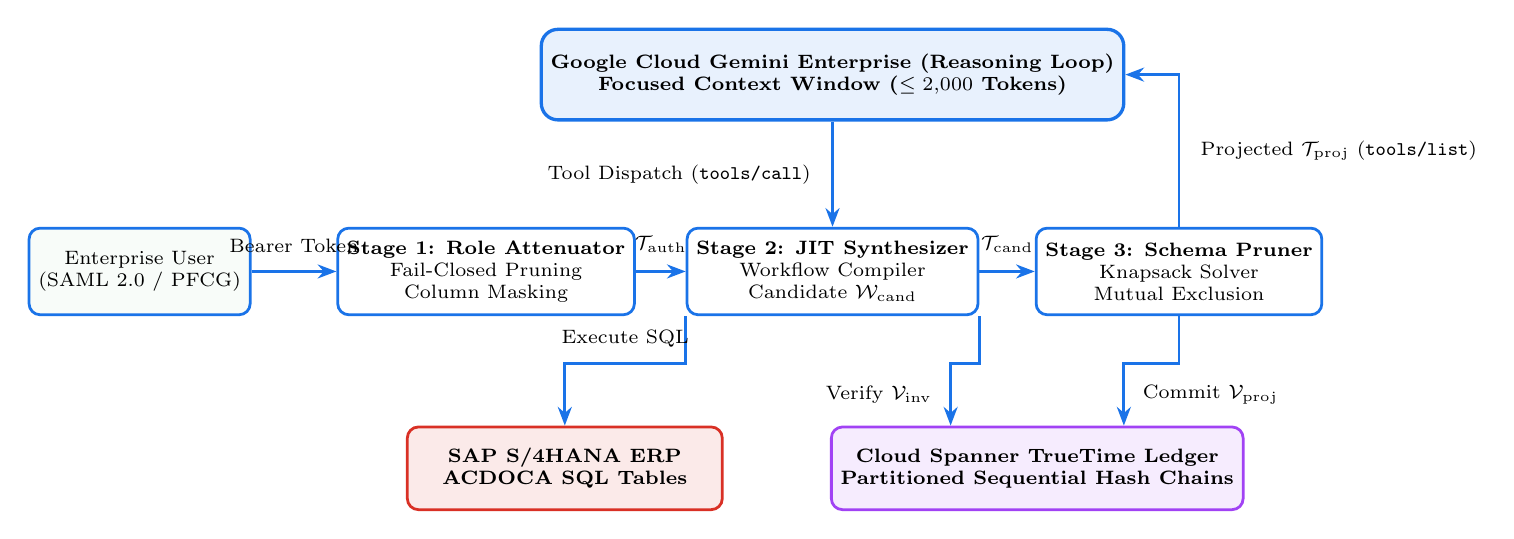
\begin{tikzpicture}[
    node distance=1.0cm and 1.5cm,
    box/.style={rectangle, draw=googleblue, fill=white, rounded corners=4pt, line width=1pt, minimum width=2.8cm, minimum height=1.1cm, align=center, font=\scriptsize},
    llmbox/.style={rectangle, draw=googleblue, fill=googleblue!10, rounded corners=6pt, line width=1.2pt, minimum width=6.6cm, minimum height=1.15cm, align=center, font=\scriptsize\bfseries},
    spannerbox/.style={rectangle, draw=googlepurple, fill=googlepurple!10, rounded corners=4pt, line width=1pt, minimum width=4.8cm, minimum height=1.05cm, align=center, font=\scriptsize\bfseries},
    erpbox/.style={rectangle, draw=googlered, fill=googlered!10, rounded corners=4pt, line width=1pt, minimum width=4.0cm, minimum height=1.05cm, align=center, font=\scriptsize\bfseries},
    arrow/.style={-{Stealth[scale=0.9]}, line width=1pt, draw=googleblue}
]

% Top Layer: LLM Reasoning Engine (Centered at x=8.8, y=2.5)
\node[llmbox] (llm) at (8.8, 2.5) {Google Cloud Gemini Enterprise (Reasoning Loop)\\Focused Context Window ($\le 2{,}000$ Tokens)};

% Middle Layer: Core Agent-JIT Pipeline (y=0) with generous 4.4cm spacing
\node[box, fill=greentint!30] (client) at (0.0, 0) {Enterprise User\\(SAML 2.0 / PFCG)};
\node[box] (attenuator) at (4.4, 0) {\textbf{Stage 1: Role Attenuator}\\Fail-Closed Pruning\\Column Masking};
\node[box] (synthesizer) at (8.8, 0) {\textbf{Stage 2: JIT Synthesizer}\\Workflow Compiler\\Candidate $\mathcal{W}_{\text{cand}}$};
\node[box] (graphpruner) at (13.2, 0) {\textbf{Stage 3: Schema Pruner}\\Knapsack Solver\\Mutual Exclusion};

% Bottom Layer: Infrastructure & Backends (y=-2.5) - Planar layout (zero crossings!)
\node[erpbox] (erp) at (5.4, -2.5) {SAP S/4HANA ERP\\ACDOCA SQL Tables};
\node[spannerbox] (spanner) at (11.4, -2.5) {Cloud Spanner TrueTime Ledger\\Partitioned Sequential Hash Chains};

% Clean Horizontal Flow (Stage 1 -> Stage 2 -> Stage 3)
\draw[arrow] (client) -- node[above=3pt, font=\scriptsize] {Bearer Token} (attenuator);
\draw[arrow] (attenuator) -- node[above=3pt, font=\scriptsize] {$\mathcal{T}_{\text{auth}}$} (synthesizer);
\draw[arrow] (synthesizer) -- node[above=3pt, font=\scriptsize] {$\mathcal{T}_{\text{cand}}$} (graphpruner);

% Clean Vertical Flow: Pruner -> LLM (tools/list)
\draw[arrow] (graphpruner.north) |- node[pos=0.25, right=4pt, font=\scriptsize] {Projected $\mathcal{T}_{\text{proj}}$ (\texttt{tools/list})} (llm.east);

% Clean Direct Vertical Flow: LLM -> Synthesizer (tools/call)
\draw[arrow] (llm.south) -- node[left=4pt, font=\scriptsize] {Tool Dispatch (\texttt{tools/call})} (synthesizer.north);

% Planar Downward Flow to ERP and Spanner (Zero crossings!)
\draw[arrow] (synthesizer.south west) -- ++(0, -0.6) -| node[pos=0.25, above=2pt, font=\scriptsize] {Execute SQL} (erp.north);
\draw[arrow] (synthesizer.south east) -- ++(0, -0.6) -| node[pos=0.75, left=3pt, font=\scriptsize] {Verify $\mathcal{V}_{\text{inv}}$} ([xshift=-1.1cm]spanner.north);
\draw[arrow] (graphpruner.south) -- ++(0, -0.6) -| node[pos=0.75, right=3pt, font=\scriptsize] {Commit $\mathcal{V}_{\text{proj}}$} ([xshift=1.1cm]spanner.north);

\end{tikzpicture}%
}
\caption{Agent-JIT System Architecture: Intercepting enterprise agent reasoning loops in Google Cloud Gemini Enterprise to dynamically project role-attenuated tool schemas, compile candidate composite wrappers ($\mathcal{W}_{\text{cand}}$), solve knapsack sub-schema optimization with mutual exclusion, and commit linearizable TrueTime audit vouchers in Cloud Spanner without conflicting communication paths or box collisions.}
\label{fig:arch}
\end{figure*}

\subsection{Principal-Propagated Role Attenuation (Stage 1)}
When an enterprise request is initiated, the caller's SAML 2.0 assertion or OAuth JWT bearer token is forwarded to the Agent-JIT engine. The principal security profile contains identity attributes, tenant boundary identifiers, and assigned SAP PFCG security roles (e.g., \texttt{Z\_FI\_AUDITOR\_READ}, \texttt{Z\_MM\_PURCHASING\_CLERK}):

\begin{definition}[Principal Authorization Matrix]
A principal $\mathcal{P}$ is defined as a tuple:
\begin{equation}
\mathcal{P} = \langle u, \tau, \mathcal{R}_{\text{pfcg}}, \mathcal{S}_{\text{auth}}, \mathcal{E}_{\text{auth}}, \mathcal{O}_{\text{auth}}, \mathcal{M}_{\text{restr}}, \mathcal{A}_{\text{auth}} \rangle
\end{equation}
where $u$ is the enterprise user ID, $\tau$ is the tenant identifier, $\mathcal{R}_{\text{pfcg}}$ is the set of assigned PFCG roles, $\mathcal{S}_{\text{auth}}$ and $\mathcal{E}_{\text{auth}}$ are authorized OData services and entity sets, $\mathcal{O}_{\text{auth}} \subseteq \{\text{READ}, \text{QUERY}, \text{CREATE}, \text{UPDATE}, \text{DELETE}, \text{EXECUTE}\}$ is the permitted operation set, $\mathcal{M}_{\text{restr}}$ is the field-level restriction mask (indexed by entity-qualified attribute keys \texttt{<Entity>.<Attr>} and global wildcards \texttt{*.<Attr>} to prevent cross-entity namespace collisions), and $\mathcal{A}_{\text{auth}} \subseteq (\mathcal{R}_{\text{pfcg}} \cup \{*\}) \times \mathcal{S} \times \mathcal{E} \times \mathcal{O}$ represents the set of coupled authorization capability tuples, with $\mathcal{S}_{\text{auth}}, \mathcal{E}_{\text{auth}}, \mathcal{O}_{\text{auth}}$ serving as marginal projections of $\mathcal{A}_{\text{auth}}$.
\end{definition}

The Role Attenuation Engine enforces two strict filtering invariants before any prompt construction. Each tool $t \in \mathcal{T}$ is formally defined by its operational signature $t = \langle \text{id}_t, r_t, \text{srv}_t, \text{ent}_t, op_t, \text{Tags}(t) \rangle$, where $r_t$ is the required PFCG role, $\text{srv}_t$ is the target OData service, $\text{ent}_t$ is the accessed entity set, $op_t \in \mathcal{O} = \{\text{READ}, \text{QUERY}, \text{CREATE}, \text{UPDATE}, \text{DELETE}, \text{EXECUTE}\}$ is the operational verb drawn from the universal operation domain, and $\text{Tags}(t)$ is the set of semantic domain tags:
\begin{enumerate}
    \item \textbf{Fail-Closed Catalog Pruning:} To prevent Cartesian-product over-approximation across disjoint domain roles, each tool's required role $r_t$ uniquely binds its operational capability $(\text{srv}_t, \text{ent}_t, op_t)$ in the catalog. A tool $t \in \mathcal{T}$ is retained in candidate set $\mathcal{T}_{\text{auth}}$ if and only if:
    \begin{equation}
    \begin{aligned}
    \exists \tilde{r} &\in ((\mathcal{R}_{\text{pfcg}} \cup \{*\}) \cap \{r_t, *\}) \\
    &\text{s.t.}\quad (\tilde{r}, \text{srv}_t, \text{ent}_t, op_t) \in \mathcal{A}_{\text{auth}}
    \end{aligned}
    \end{equation}
    Any tool violating this condition is evicted. Administrative endpoints (e.g., F110 automated payment disbursement or user role escalation) are eliminated from the search space. Stage 1 guarantees fail-closed containment across services, entity sets, and field properties; row-level organizational criteria (e.g., Company Code \texttt{BUKRS} or Plant \texttt{WERKS}) are enforced downstream via token propagation or parameter inspection.
    \item \textbf{Column-Level Schema Masking:} For each tool $t$, let $\mathcal{M}_{\text{restr}}(t) \triangleq \{k \mid \text{ent}_t.k \in \mathcal{M}_{\text{restr}} \lor \texttt{*.}k \in \mathcal{M}_{\text{restr}}\}$ denote its entity-resolved attribute restriction projection. Partitioning input parameters into mandatory/key parameters and optional filter parameters, $\text{Params}(t) = \text{Params}_{\text{req}}(t) \cup \text{Params}_{\text{opt}}(t)$, if any mandatory input or primary-key lookup attribute is restricted ($\operatorname{dom}(\text{Params}_{\text{req}}(t)) \cap \mathcal{M}_{\text{restr}}(t) \neq \emptyset$), the Role Attenuation Engine fails closed by evicting the entire tool $t$ from $\mathcal{T}_{\text{auth}}$, preventing downstream HTTP 400 schema validation failures. Otherwise, for each retained $t \in \mathcal{T}_{\text{auth}}$, $\text{Params}(t)$ and output schemas $\text{Out}(t)$ are projected to strip restricted attributes:
    \begin{equation}
    \begin{aligned}
    \text{Params}'(t) &= \{ (k, v) \in \text{Params}(t) \mid k \notin \mathcal{M}_{\text{restr}}(t) \}, \\
    \text{Out}'(t) &= \{ (k, v) \in \text{Out}(t) \mid k \notin \mathcal{M}_{\text{restr}}(t) \}
    \end{aligned}
    \end{equation}
    with $\text{Props}'(t) \triangleq \text{Params}'(t) \cup \text{Out}'(t)$ denoting the union of projected property sets. For analytical query tools and optional parameters, restricted fields (such as employee payroll masks \texttt{EmployeeSalaryMask} or confidential bank IBANs) are masked from property definitions and return schemas, preventing LLM awareness of confidential fields.
\end{enumerate}

\subsection{Just-In-Time Composite Tool Synthesis (Stage 2)}
When an incoming query implies a multi-hop relational workflow—such as cross-entity reconciliation, master-detail verification, or multi-step transactional posting—executing the query via atomic tools requires multiple sequential LLM conversational round trips.

Agent-JIT incorporates an in-memory Abstract Syntax Tree (AST) workflow compiler that evaluates candidate workflows over authorized tools $\mathcal{T}_{\text{auth}}$ (throughout, $\mathcal{W}$ and $\mathcal{W}_{\text{comp}}$ are used interchangeably to denote a candidate composite wrapper in $\mathcal{W}_{\text{cand}}$, and $V_E^{\text{auth}} \triangleq \{\text{ent}_t \mid t \in \mathcal{T}_{\text{auth}}\}$ denotes the subset of entities possessing at least one authorized tool). To bridge Stages 2 and 3 deterministically without circular dependencies: initial lexical-semantic scores $S_0(t, q)$ (Eqs.~(\ref{eq:initial_score})--(\ref{eq:bm25})) are evaluated first across $\mathcal{T}_{\text{auth}}$, yielding initial seed entities $\operatorname{Seeds}_0(q)$ as the top-$K_{\text{seed}} = 5$ elements of $\{e \in V_E^{\text{auth}} \mid \max_{t \in \mathcal{T}_{\text{auth}} : e \in \operatorname{Entities}(t)} S_0(t, q) > \theta\}$ ranked by $\max_{t \in \mathcal{T}_{\text{auth}} : e \in \operatorname{Entities}(t)} S_0(t, q)$ with deterministic entity-level tie-breaking by ascending lexicographical entity identifier $e \in V_E^{\text{auth}}$ across $\operatorname{Seeds}_0(q)$, $\operatorname{Seeds}_1(q)$, and $\operatorname{Seeds}(q)$ (when $|\operatorname{Seeds}_0(q)| = 0$, Stage 2 synthesis and Stage 3 multigraph propagation are bypassed so $S(t, q) = S_0(t, q)$). When $|\operatorname{Seeds}_0(q)| \ge 2$, Stage 3 multigraph propagation (Eq.~(\ref{eq:propagation})) executes with horizon $h_{\max} = 1$ and $\operatorname{Seeds}(q) = \operatorname{Seeds}_0(q)$, compiling matched declarative templates or—when no declarative template matches—executing dynamic BFS pathfinding over $\operatorname{Seeds}_0(q)$ in Stage 2 (if all matched declarative templates or a 2-hop ad-hoc BFS wrapper connecting two seeds via an unseeded intermediate bridge entity $e_2 \in V_E^{\text{auth}} \setminus \operatorname{Seeds}_0(q)$ subsequently fail Stage 2 compilation or Stage 3 budget feasibility, dynamic BFS pathfinding and $h_{\max} = 2$ propagation execute as a fallback with a single Stage 3 greedy pass restart so $e_2$'s atomic tools receive 1-hop amplification). When $|\operatorname{Seeds}_0(q)| = 1$, the engine first executes an $h_{\max} = 1$ pass (expanding $\operatorname{Seeds}_1(q)$ by appending up to $K_{\text{seed}} - 1 = 4$ top 1-hop entities $e_2 \in V_E^{\text{auth}}$ ranked by $\max_{t' \in \mathcal{T}_{\text{auth}} : e_2 \in \operatorname{Entities}(t')} S(t', q) > \theta_1$, where $\theta_h \triangleq \gamma^h \theta$ denotes the hop-decay-scaled admissibility threshold with $\theta_1 = 0.20$ for $h=1$ and $\theta_2 = 0.10$ for $h=2$, automatically satisfied whenever the anchor seed tool $t_1^*$ satisfies $S_0(t_1^*, q) > \theta = 0.40$ since $\gamma^h S_0(t_1^*, q) > \gamma^h \theta = \theta_h$, while candidate ranking among $e_2, e_3$ nodes is differentiated by their baseline lexical-semantic scores $S_0(t_2, q), S_0(t_3, q)$ and exceeds unscaled $\theta = 0.40$ whenever $S_0(t_{h+1}, q) > \theta - \gamma^h S_0(t_1^*, q)$) and evaluates declarative template triggers over $\operatorname{Seeds}_1(q)$; if no declarative template matches—or if all matched declarative templates are subsequently pruned fail-closed during Stage 2 compilation or rejected due to budget constraints (evaluated both statically at the end of Stage 2 when $\text{Cost}(\mathcal{W}) > B$ and dynamically upon residual budget exhaustion $\Phi(\mathcal{T}_{\text{proj}}) + \Delta C > B$ in Stage 3, where $\text{Cost}(\mathcal{W})$ and $\Delta C = \text{Cost}(\mathcal{W}) - \sum_{c' \in \operatorname{Evicted}(\mathcal{W})} \text{Cost}(c')$ are formally defined in Section~II-C with $\Delta C = \text{Cost}(\mathcal{W})$ when $\operatorname{Evicted}(\mathcal{W}) = \emptyset$ during Forward Blocking; dynamic exhaustion of all matched templates in Stage 3 triggers $h_{\max} = 2$ multigraph propagation, updates $S(\mathcal{W}, q)$ for any budget-deferred templates alongside atomic tools under the $h_{\max} = 2$ scores $S(t_k, q)$, compiles any fallback dynamic BFS candidates over $\operatorname{Seeds}(q)$, and restarts the Stage 3 greedy pass by re-sorting $\mathcal{T}_{\text{cand}}$ under the updated $h_{\max} = 2$ value densities $S(c, q)/\text{Cost}(c)$ at most once per query, preserving $O(|\mathcal{T}_{\text{cand}}| \log |\mathcal{T}_{\text{cand}}|)$ time complexity while ensuring hop-2 constituent atomic tools $t_3$ receive $\gamma^2 = 0.25$ amplification prior to atomic fallback admission)—the engine first re-evaluates Eq.~(\ref{eq:propagation}) with $h_{\max} = 2$ across $\mathcal{T}_{\text{auth}}$ with geometric decay $\gamma^h$ ($\gamma = 0.5, \gamma^2 = 0.25$) and then constructs $\operatorname{Seeds}(q)$ by allocating the $K_{\text{seed}} - 1 = 4$ expansion slots in $\operatorname{Seeds}(q)$ ($|\operatorname{Seeds}(q)| \le 5$, bounding seed pairs to at most $\binom{5}{2} = 10$): reserving up to $2$ slots for the highest-scoring $h=1$ neighbors $e_2 \in V_E^{\text{auth}}$ and up to $2$ slots for the highest-scoring $h=2$ neighbors $e_3 \in V_E^{\text{auth}}$ reachable along top-scoring 2-hop shortest-path chains $e_1 \to e_2 \to e_3$ over the symmetric closure (undirected projection) of $E_N$ oriented outward from $e_1$ through an authorized intermediate bridge entity $e_2 \in V_E^{\text{auth}}$ and ranked by cumulative post-propagation chain score $\max_{t_2 \in \mathcal{T}_{\text{auth}} : e_2 \in \operatorname{Entities}(t_2)} S(t_2, q) + \max_{t_3 \in \mathcal{T}_{\text{auth}} : e_3 \in \operatorname{Entities}(t_3)} S(t_3, q)$ with $e_2, e_3$ exceeding their respective hop-scaled thresholds $\theta_1, \theta_2$ and lexicographical tie-breaking on $(e_2, e_3)$ (if a selected chain's intermediate entity $e_2$ is not already among the top-2 standalone $h=1$ slots, $e_2$ replaces the lowest-ranked remaining standalone $h=1$ slot without evicting any bridge entity already locked in by a higher-ranked $h=2$ chain, so both $e_2$ and $e_3$ are guaranteed to enter $\operatorname{Seeds}(q)$ for ad-hoc BFS and atomic fallback scoring even when $e_1$ has $\ge 4$ 1-hop neighbors, while any unused $h=2$ or $h=1$ slots roll over to admit additional qualifying neighbors up to $K_{\text{seed}} = 5$). (i) \emph{Declarative Template Triggering:} For structured enterprise workflows (such as AP 3-way matching or Order-to-Cash fulfillment), a pre-registered declarative template $\mathcal{W}$ is instantiated whenever at least two of its constituent entities belong to the active seed set ($\operatorname{Seeds}_1(q)$ or $\operatorname{Seeds}(q)$), or when a single designated anchor entity belongs to $\operatorname{Seeds}_0(q)$ and the query matches multi-step workflow intent tokens ($\operatorname{IntentTokens}(\mathcal{W}) \cap \operatorname{Tokens}(q) \neq \emptyset$, e.g., \texttt{reconcile}, \texttt{3-way}, \texttt{match}, \texttt{verify}, \texttt{fulfill}, enabling single-seed workflow queries such as ``reconcile invoice INV-2026'' to instantiate the 3-step template while preventing false-positive template triggering on purely single-entity atomic lookups); in Eq.~(8), all constituent steps use the active Stage 3 score $S(t_k, q)$ from Eq.~(\ref{eq:propagation}) (so on a single-seed query $|\operatorname{Seeds}_0(q)| = 1$ under an admitted template with $h_{\max}=1$ where $t_3$ is 2 hops from the sole anchor seed, $t_3$ contributes $S(t_3, q) = S_0(t_3, q)$ since the intermediate 1-hop tool $t_2$ satisfies $S_0(t_2, q) \le \theta$, while $t_2$ receives 1-hop amplification, foreign-key parameter elimination reduces $\text{Cost}(\mathcal{W})$, and the wrapper receives $\Delta_{\text{comp}} = 0.25$—which together already place $\frac{S(\mathcal{W}, q)}{\text{Cost}(\mathcal{W})}$ above constituent atomic densities without requiring spurious $\gamma^2$ amplification of unrelated 2-hop tools unless budget exhaustion triggers the $h_{\max}=2$ restart). (ii) \emph{Dynamic BFS \& Entity-to-Tool Inverse Mapping:} For ad-hoc read-only analytical queries where no declarative template matches (or where matched templates fail compilation/budget feasibility), the synthesizer triggers dynamic BFS pathfinding over the symmetric closure (undirected projection) of navigation edges $E_N$ when $|\operatorname{Seeds}(q)| \ge 2$, discovering minimal-hop relational paths ($m \le 3$) connecting seed pairs with distinct constituent tools ($t_j \neq t_k$ for $j \neq k$, preventing cyclic tool self-joins while permitting self-referential foreign-key associations $(e, e) \in E_N$ or 2-hop paths $e_1 \to e_2 \to e_1$ that visit the same entity $e_j = e_k$ via distinct tools $t_j \neq t_k$—such as a single-record \texttt{READ} lookup followed by a collection \texttt{QUERY}—and orienting the execution pipeline $\vec{\sigma} = \langle \sigma_1, \dots, \sigma_m \rangle$ outward from the highest-$S_0$ anchor seed entity) and coalescing pairs of strict 2-entity (1-hop) seed-pair sub-paths $(e_1, e_2)$ and $(e_2, e_3)$ into maximal $m=3$-entity (2-hop) chains when all three entities belong to $\operatorname{Seeds}(q)$ (whereas a direct minimal 2-hop path $e_1 \to e_2 \to e_3$ connecting two non-adjacent seeds $e_1, e_3 \in \operatorname{Seeds}(q)$ at shortest distance 2 in the symmetric closure of $E_N$ may traverse an unseeded intermediate bridge entity $e_2 \in V_E^{\text{auth}} \setminus \operatorname{Seeds}(q)$ provided $e_2$ possesses an authorized tool in $\mathcal{T}_{\text{auth}}$). Each traversed entity $e_k$ is mapped deterministically to an authorized read-only tool $\text{ToolID}_k \in \mathcal{T}_{\text{auth}}$: when upstream step $k-1$ returns a single entity record ($1\text{:}1$ or $N\text{:}1$ association from a \texttt{READ} tool $t_{k-1}$), step $k$ selects a single-entity \texttt{READ} key-lookup tool whenever the upstream \texttt{<ReferentialConstraint>} foreign-key binding fully covers the target tool's mandatory key parameters ($\operatorname{dom}(\text{Params}_{\text{req}}(t_k)) \subseteq \operatorname{BoundFK}(\sigma_k)$), and falls back to a collection-filtering \texttt{QUERY} tool retaining all bound foreign-key filter attributes ($\operatorname{BoundFK}(\sigma_k) \subseteq \operatorname{dom}(\text{Params}'(t_k))$) whenever an upstream binding covers only a partial compound-key prefix; conversely, when upstream step $k-1$ returns a collection (either because $t_{k-1}$ is a \texttt{QUERY} tool or the association has $1\text{:}N$ cardinality), step $k$ preferentially selects a collection-filtering \texttt{QUERY} tool ($\operatorname{BoundFK}(\sigma_k) \subseteq \operatorname{dom}(\text{Params}'(t_k))$) for disjunctive OData \texttt{\$filter} set pushdown (or intra-service \texttt{\$expand}), and falls back to bounded OData \texttt{\$batch} key-lookup fan-out ($\le K_{\text{fanout}} = 50$ deduplicated keys) over a single-entity \texttt{READ} tool $t_k$ only when no authorized \texttt{QUERY} tool exists on $e_k$ and $\operatorname{dom}(\text{Params}_{\text{req}}(t_k)) \subseteq \operatorname{BoundFK}(\sigma_k)$, breaking ties in all cases by highest $S_0(t, q)$ and then lexicographical $\text{id}_t$ (when an unseeded intermediate bridge entity $e_2 \notin \operatorname{Seeds}_0(q)$ exposes multiple authorized \texttt{QUERY} tools representing distinct business views or status filters---such as open vs.\ cleared items---that share identical primary/foreign-key signatures and near-identical baseline scores $|S_0(t_a, q) - S_0(t_b, q)| \le \epsilon_{\text{view}} = 0.02$, the compiler selects the unfiltered canonical base-entity view, identified via the OData CSDL \texttt{DefaultView} annotation or absence of a static \texttt{\$filter} restriction, for the composite bridge step while retaining the specialized view variants as independent atomic candidates in $\mathcal{T}_{\text{cand}}$); if any intermediate entity $e_k$ lacks an authorized tool in $\mathcal{T}_{\text{auth}}$ satisfying the required binding modality, the path fails closed. (iii) \emph{Semantic Disambiguation Across Equi-Length Foreign-Key Paths:} Property-level foreign-key bindings are extracted from OData CSDL~\cite{pizzo2020odata} \texttt{<ReferentialConstraint>} metadata (\texttt{PrincipalRole} and \texttt{DependentRole}). When two seed entities are connected by multiple authorized minimal-hop paths with distinct business role semantics (e.g., \texttt{CreatedBy} vs.\ \texttt{ApprovedBy} or \texttt{BillTo} vs.\ \texttt{ShipTo}), all valid minimal paths are compiled into $\mathcal{W}_{\text{cand}}$ and disambiguated by a bounded query-conditioned role-alignment term $\delta_{\text{fk}}(\mathcal{W}, q) = \min(0.15, 0.05 \cdot |\operatorname{RoleTokens}(\mathcal{W}) \cap \operatorname{Tokens}(q)|)$ added to $S(\mathcal{W}, q)$ in Eq.~(8), where $\operatorname{RoleTokens}(\mathcal{W})$ normalizes the CSDL \texttt{NavigationProperty} and \texttt{DependentRole} identifiers. Furthermore, Stage 2 constructs unified parameter and output schemas deterministically as $\text{Params}_{\text{unified}}(\mathcal{W}_{\text{comp}}) \triangleq \operatorname{Prefix}_1(\operatorname{Params}'(t_1)) \cup \bigcup_{k=2}^m \operatorname{Prefix}_k(\{(k_{\text{p}}, v) \in \operatorname{Params}'(t_k) \mid k_{\text{p}} \notin \operatorname{BoundFK}(\sigma_k)\})$ (where any unbound mandatory parameters in $\{(k_{\text{p}}, v) \in \operatorname{Params}_{\text{req}}(t_k) \mid k_{\text{p}} \notin \operatorname{BoundFK}(\sigma_k)\}$ retain their \texttt{required} schema status under $\operatorname{Prefix}_k(\cdot)$) and $\text{Out}'(\mathcal{W}_{\text{comp}}) \triangleq \bigcup_{k=1}^m \operatorname{Prefix}_k(\operatorname{Out}'(t_k))$—where $\operatorname{Prefix}_k(\cdot)$ applies entity-qualified renaming \texttt{<Entity>\_<Attr>} (or step-and-entity-qualified \texttt{S<k>\_<Entity>\_<Attr>} strictly when an attribute $a \in \operatorname{Props}'(t_k)$ collides with another step $j \neq k$ that accesses the same entity set, $\text{ent}_{t_j} = \text{ent}_{t_k}$, whereas if all colliding steps $j \neq k$ access distinct entity sets $\text{ent}_{t_j} \neq \text{ent}_{t_k}$, entity-qualified \texttt{<Entity>\_<Attr>} already disambiguates the collision) prior to set union whenever an attribute name in $\operatorname{Props}'(t_k)$ collides with the combined domain $\bigcup_{j \neq k} (\operatorname{dom}(\operatorname{Props}'(t_j)) \cup \mathcal{M}_{\text{restr}}(t_j))$ of any other constituent step—strictly over Stage 1 pre-masked schemas, with unified composite restriction mask $\mathcal{M}_{\text{restr}}(\mathcal{W}_{\text{comp}}) \triangleq \bigcup_{k=1}^m \operatorname{Prefix}_k^{\text{all}}(\mathcal{M}_{\text{restr}}(t_k))$ (where $\operatorname{Prefix}_k^{\text{all}}(\cdot)$ evaluates the identical collision trigger once against the combined domain $\bigcup_{j \neq k} (\operatorname{dom}(\operatorname{Props}'(t_j)) \cup \mathcal{M}_{\text{restr}}(t_j))$ so an unrestricted attribute $a$ on step $j$ never falsely collides with a restricted attribute $a \in \mathcal{M}_{\text{restr}}(t_k)$ on step $k\neq j$). If for any bound foreign-key join pair $(k_{\text{src}}, k_{\text{tgt}})$ in $\sigma_k$ either the upstream source attribute or downstream target parameter is masked ($k_{\text{src}} \in \mathcal{M}_{\text{restr}}(t_{k-1}) \lor k_{\text{tgt}} \in \mathcal{M}_{\text{restr}}(t_k)$), any workflow-required parameter of a compensating action $\operatorname{Comp}(\sigma_k)$ (including parameters that are optional in $\operatorname{Params}_{\text{opt}}(\operatorname{Comp}(t_k))$ for standalone calls and thus survived Stage 1, but are mandatory to reverse $\sigma_k$) lies in $\mathcal{M}_{\text{restr}}(\operatorname{Comp}(t_k))$, or any forward output attribute in $\operatorname{Out}(t_k)$ required to parameterize $\operatorname{Comp}(\sigma_k)$ lies in $\mathcal{M}_{\text{restr}}(t_k)$, the engine prunes that candidate and fails closed.

To guarantee complete operational containment, let the Boolean predicate $\operatorname{NeedsSagaComp}(\sigma_k)$ indicate whether $\sigma_k$ is a mutating step executing outside a single-service atomic OData \texttt{\$batch} changeset (whereas intra-changeset mutating steps roll back atomically via native \texttt{ROLLBACK WORK} with $\operatorname{Comp}(\sigma_k) = \text{null}$); a composite wrapper $\mathcal{W}_{\text{comp}} \in \mathcal{W}_{\text{cand}}$ is compiled if and only if all forward constituent steps and all required Saga compensating actions reside within $\mathcal{T}_{\text{auth}}(\mathcal{P})$:
\begin{equation}
\mathcal{W}_{\text{comp}} = \langle \text{ID}_{\text{comp}}, \text{Name}, \text{Params}_{\text{unified}}, \vec{\sigma}, \mathcal{R}_{\cup}, \mathcal{H}_{\text{ast}} \rangle
\end{equation}
where $\vec{\sigma} = \langle \sigma_1, \sigma_2, \dots, \sigma_m \rangle$ is an ordered pipeline of atomic tool invocations with dynamic parameter bindings:
\begin{equation}
\sigma_k : \text{ToolID}_k(\text{Args}_k) \quad \text{where} \quad \text{Args}_k \leftarrow f(\text{Input}, \text{Output}_{<k})
\end{equation}
For $1\text{:}N$ or collection-returning upstream steps, $f(\text{Input}, \text{Output}_{<k})$ binds intermediate entity sets via OData \texttt{\$expand} join pushdown for intra-service read queries, and disjunctive \texttt{\$filter} set predicates on collection \texttt{QUERY} tools (or bounded OData \texttt{\$batch} key-lookup fan-out $\le K_{\text{fanout}} = 50$ on \texttt{READ} tools when no \texttt{QUERY} tool is authorized) for cross-service steps. For each step $\sigma_k$ in Equation~(5), let $t_k \in \mathcal{T}_{\text{auth}}$ denote the invoked atomic tool and $r_{\sigma_k}$ its required PFCG role in Equation~(6), where $\mathcal{R}_{\cup}$ aggregates required roles across both forward and Saga-compensated operations:
\begin{equation}
\mathcal{R}_{\cup} \triangleq \bigcup_{k=1}^m \Big( \{r_{\sigma_k}\} \cup \{r_{\text{Comp}(\sigma_k)} \mid \operatorname{NeedsSagaComp}(\sigma_k)\} \Big)
\end{equation}
and $\mathcal{H}_{\text{ast}}$ is a deterministic SHA-256 fingerprint binding both forward and backward operational structures (with $\operatorname{Comp}(\vec{\sigma}) \triangleq \langle \operatorname{Comp}(\sigma_m), \dots, \operatorname{Comp}(\sigma_1) \rangle$, where $\operatorname{Comp}(\sigma_k) = \text{null}$ for read-only and single-changeset \texttt{ROLLBACK WORK} steps):
\begin{equation}
\begin{aligned}
\mathcal{H}_{\text{ast}} = \operatorname{SHA-256}\Big(&\operatorname{CanonicalJSON}(\vec{\sigma}) \\
&\parallel \operatorname{CanonicalJSON}(\text{Comp}(\vec{\sigma})) \\
&\parallel \operatorname{CanonicalJSON}(\operatorname{Sort}(\mathcal{R}_{\cup}))\Big)
\end{aligned}
\end{equation}
Compiled candidate composite wrappers form the set $\mathcal{W}_{\text{cand}}$, which expands the candidate pool for Stage 3 knapsack projection: $\mathcal{T}_{\text{cand}} \triangleq \mathcal{T}_{\text{auth}} \cup \mathcal{W}_{\text{cand}}$. For each composite wrapper $\mathcal{W} \in \mathcal{W}_{\text{cand}}$, its relevance utility is defined super-additively over its forward constituent steps $\text{Constituents}_{\text{fwd}}(\mathcal{W}) \triangleq \{t_k \mid k \in \{1, \dots, m\}\}$:
\begin{equation}
\label{eq:comp_score}
S(\mathcal{W}, q) \triangleq \sum_{t \in \text{Constituents}_{\text{fwd}}(\mathcal{W})} S(t, q) + \Delta_{\text{comp}} + \delta_{\text{fk}}(\mathcal{W}, q)
\end{equation}
where $S(t, q)$ is the multigraph-amplified relevance score formally defined in Stage 3 (Eq.~(\ref{eq:propagation})) and $\Delta_{\text{comp}} = 0.25$ is the composition utility bonus, guaranteeing that admitting $\mathcal{W}$ yields higher objective utility than individual constituent tools when feasible under budget $B$.

When the LLM invokes $\mathcal{W}_{\text{comp}}$, the Agent-JIT runtime executes the constituent OData operations sequentially within the server process against physical database tables, passing intermediate keys without returning to the model between steps.

\textbf{Transactional Failure Semantics \& Non-Compensable Boundaries:} In multi-step mutating workflows, single-endpoint transaction batches execute within native SAP OData \$batch changesets, rolling back atomically via \texttt{ROLLBACK WORK} on failure. For multi-request distributed pipelines, the execution engine coordinates backward compensating operations following classical Saga protocols~\cite{garciamolina1987sagas, mohan1992aries}, executing pre-registered inverse actions $\text{Comp}(\sigma_k)$ (e.g., reversing journal postings or releasing reservation locks) to restore backend consistency; if a compensating action $\operatorname{Comp}(\sigma_k)$ encounters a transient network drop or row-lock timeout during rollback, the engine executes bounded exponential-backoff retries ($3$ attempts over $10$~ms--$50$~ms carrying deterministic idempotency key \texttt{c\_idemp}), and if retries exhaust, persists a dead-letter recovery record (\texttt{COMPENSATION\_FAILED\_DLQ}) in Cloud Spanner / SQLite WAL while retaining the \texttt{PROVISIONAL\_PENDING} quarantine lock and escalating a high-priority PagerDuty / SAP Solution Manager administrative alert. To prevent dirty reads across concurrent MCP sessions during the $<15$~ms local fault-recovery window (or $45$--$110$~ms over remote OData v4 endpoints) prior to $\operatorname{Comp}(\sigma_1)$, intermediate steps tag records with a provisional state (\texttt{Status = PROVISIONAL\_PENDING}) that is excluded by default in Agent-JIT read projections until the final step commits. In hybrid deployments where external non-MCP SAP transactions (such as direct SAP GUI sessions or background ABAP batch jobs) query underlying ERP tables concurrently without routing through Agent-JIT's middleware filter, native cross-application dirty-read isolation applies to ERP business objects that expose native parked document states (e.g., SAP \texttt{BAPI\_ACC\_DOCUMENT\_POST} parked status \texttt{VSTAT = 'V'}) or S/4HANA RAP Draft Administrative Data staging tables (\texttt{I\_DraftAdministrativeData}), as well as single-service OData \texttt{\$batch} changesets, so uncommitted intermediate records remain invisible to native ABAP/GUI readers until final step completion promotes them to posted status; conversely, for arbitrary cross-service mutating REST/OData endpoints or legacy BAPIs that commit immediately upon HTTP \texttt{POST}/\texttt{PATCH} without native draft or parked states, strict read isolation is guaranteed across all Agent-JIT MCP sessions via \texttt{PROVISIONAL\_PENDING} filtering, whereas unmediated external non-MCP database readers observe standard Saga eventual consistency (transient visibility of intermediate step commits during the $13.8$~ms local or $45$--$110$~ms remote rollback window until $\operatorname{Comp}(\sigma_k)$ completes; to prevent classic Saga lost-update hazards if an unmediated external non-MCP transaction concurrently modifies the intermediate record during this $13.8$~ms local or $45$--$110$~ms remote rollback window, each forward step $\sigma_k$ captures the post-mutation HTTP response \texttt{ETag} [or SAP change-document watermark \texttt{CHANGE\_NR} / post-image attribute digest] and $\operatorname{Comp}(\sigma_k)$ attaches an optimistic concurrency precondition [\texttt{If-Match: <ETag>} or BAPI state-precondition diff check] during rollback, failing closed into a dedicated \texttt{COMPENSATION\_CONFLICT\_DLQ} state for human/exception reconciliation rather than overwriting the concurrent external update). For read-only reconciliation queries (such as AP 3-way matching), the pipeline performs relational join pushdown across foreign-key navigation paths, aggregating results in a single turn without intermediate LLM round trips and without requiring compensating database mutations. For non-compensable actions with irreversible real-world physical side effects (such as settled external SWIFT/Fedwire wire transfers), the engine validates all input preconditions and suspends automated execution prior to dispatching $\sigma_1$ (avoiding uncommitted mid-pipeline locks during human approval waits), returning an intermediate task token $\tau_{\text{task}}$ with status \texttt{PENDING\_AUTHORIZATION} and requiring out-of-band dual-custody human sign-off before execution.

\subsection{Goal-Conditioned Sub-Schema Pruning (Stage 3)}
Following role attenuation and candidate composite wrapper compilation, the candidate pool $\mathcal{T}_{\text{cand}} = \mathcal{T}_{\text{auth}} \cup \mathcal{W}_{\text{cand}}$ may contain hundreds of authorized atomic and composite tools. The Schema Pruner selects the most goal-relevant tools subject to a token budget constraint $B$ (default $B = 2{,}000$ tokens).

\begin{definition}[Heterogeneous Capability Multigraph]
Let $G = (V_T \cup V_E, E_R \cup E_N)$ be a heterogeneous capability multigraph where $V_T \equiv \mathcal{T}_{\text{auth}}$ is the set of authorized tools, $V_E$ is the set of OData entity sets, $E_R \subseteq V_T \times V_E$ represents bipartite tool-entity operational bindings, and $E_N \subseteq V_E \times V_E$ represents directional navigation associations (foreign key relationships) between entities.
\end{definition}

In compliance with the Model Context Protocol (MCP) JSON-RPC 2.0 specification, caller natural language goal $q$ and identity assertions are conveyed via standard protocol parameter extensions (under \texttt{params.\_meta.user\_goal} or session transport headers \texttt{X-Agent-Goal}). For goal $q$, the engine computes an initial semantic relevance score $S_0(t, q)$ combining dampened maximum-scaled BM25 lexical token matching and continuous dense semantic embeddings $\mathbf{e}_q, \mathbf{e}_t \in \mathbb{R}^d$:
\begin{equation}
\label{eq:initial_score}
\begin{aligned}
S_0(t, q) = \beta &\cdot \widehat{\mathrm{BM25}}(q, \text{Doc}(t)) \\
&+ (1 - \beta) \cdot \max(0, \cos(\mathbf{e}_q, \mathbf{e}_t)) \\
&+ \alpha \cdot \mathbf{1}_{\{\text{Tags}(t) \cap \text{Tokens}(q) \neq \emptyset\}}
\end{aligned}
\end{equation}
where $\text{Doc}(t)$ concatenates tool name, description, and strictly the Stage 1 pre-masked schema properties $\text{Props}'(t)$ (excluding restricted attributes in $\mathcal{M}_{\text{restr}}(t)$ so masked fields never influence ranking), $\text{Tokens}(q)$ denotes all lowercased alphanumeric query tokens after stopword removal normalized under the same convention as $\text{Tags}(t)$, $\beta = 0.5$ balances lexical and semantic density, $\alpha = 0.35$ is the semantic category bonus weight, $\text{BM25}(q, \text{Doc}(t)) \triangleq \min\big(1, \text{BM25}_{\text{raw}}(q, \text{Doc}(t)) / Z_{\text{BM25}}(q)\big) \in [0, 1]$ denotes the clamped pre-normalized Okapi BM25 score ($k_1 = 1.5, b = 0.75$, using non-negative Lucene/Robertson inverse document frequency $\text{IDF}(w) = \ln\!\big(1 + \frac{|\mathcal{T}| - n_w + 0.5}{n_w + 0.5}\big) > 0$—where $n_w$ is the number of tools in $\mathcal{T}$ whose $\text{Doc}(t)$ contains token $w$—and mean document token length $\text{avgdl}$ precomputed offline across $\mathcal{T}$) divided by the query's theoretical upper bound $Z_{\text{BM25}}(q) \triangleq \max\big(2 \cdot \text{IDF}_{\text{med}}, \sum_{w \in \operatorname{Tokens}(q)} \text{IDF}(w) \cdot (k_1 + 1)\big)$ (where $\text{IDF}_{\text{med}}$ is the median $\text{IDF}(w)$ precomputed offline across all unique vocabulary tokens in the full catalog $\mathcal{T}$, and $2 \cdot \text{IDF}_{\text{med}}$ serves as a two-term median-IDF floor ensuring a low-to-moderate IDF single-token hit [$\text{IDF}(w) < \frac{2}{k_1 + 1}\text{IDF}_{\text{med}} = 0.8 \cdot \text{IDF}_{\text{med}}$] cannot self-normalize to $1.0$, while high-IDF single-token hits [$\text{IDF}(w) \ge 0.8 \cdot \text{IDF}_{\text{med}}$] are capped below $\frac{1}{1 + k_{\text{sat}}} = \frac{2}{3}$ by $k_{\text{sat}}$ in Eq.~(\ref{eq:bm25})), and dampened catalog-max scaling with soft saturation constant $k_{\text{sat}} = 0.50$ and zero-clamping is defined as:
\begin{equation}
\label{eq:bm25}
\begin{aligned}
\widehat{\mathrm{BM25}}(q, \text{Doc}(t)) &\triangleq \mathbf{1}_{\{\text{BM25}(q, \text{Doc}(t)) \ge \tau_{\text{floor}}\}} \\
\cdot \max\Biggl(0, &\frac{\text{BM25}(q, \text{Doc}(t))}{\max_{t' \in \mathcal{T}_{\text{auth}}} \text{BM25}(q, \text{Doc}(t')) + k_{\text{sat}} + \epsilon}\Biggr)
\end{aligned}
\end{equation}
with calibrated normalized score floor $\tau_{\text{floor}} = 0.10$, soft saturation constant $k_{\text{sat}} = 0.50$ (which eliminates step discontinuities when $\max_{t'} \text{BM25}(q, \text{Doc}(t')) \approx \tau_{\text{floor}}$, damping a boundary single-token hit at $\text{BM25} \approx \tau_{\text{floor}}$ to $\le 0.17$, whereas even a high-IDF hit reaching $\text{BM25} = 1.0$ is capped at \mbox{$\widehat{\mathrm{BM25}} < \frac{1}{1 + k_{\text{sat}}} = \frac{2}{3} \approx 0.67$} so its weighted lexical contribution \mbox{$\beta \cdot \widehat{\mathrm{BM25}} < 0.334$} still cannot unilaterally exceed $\theta = 0.40$ without semantic or tag corroboration), and $\epsilon = 10^{-6}$, ensuring a tight dampened range \mbox{$\widehat{\mathrm{BM25}}(q, \text{Doc}(t)) \in [0, \frac{2}{3}) \subset [0, 1)$} and $S_0(t, q) \in [0, 1.18\overline{3})$ (bounded above by the nominal undampened ceiling $0.5 + 0.5 + 0.35 = 1.35$), with $\theta = 0.40$ acting as a calibrated propagation filter.

To account for relational entity context across multiple upstream dependencies, relevance scores are propagated across the capability multigraph $G$ up to horizon $h_{\max} \in \{1, 2\}$ hops with geometric decay $\gamma^h$ ($\gamma = 0.5$). For any tool $t$ with $S_0(t, q) > \theta$, the engine traverses navigation edges $E_N$ up to $h \in \{1, \dots, h_{\max}\}$ hops (where $h_{\max} = 1$ in standard multi-seed or admitted template-matched composite mode, and $h_{\max} = 2$ on single-seed queries where no declarative template is admitted as well as in atomic-only mode where Stage 2 is disabled):
\begin{equation}
\label{eq:propagation}
\begin{aligned}
S(t', q) &= S_0(t', q) + \max_{h \in \{1, \dots, h_{\max}\}} \gamma^h \\
&\quad \cdot \max\Biggl(0, \max_{\substack{t \in \mathcal{T}_{\text{auth}} \\ \text{Entities}(t) \cap \text{Adj}_h(\text{Entities}(t')) \neq \emptyset \\ S_0(t, q) > \theta}} S_0(t, q)\Biggr)
\end{aligned}
\end{equation}
where $\text{Entities}(t) \triangleq \{e \in V_E^{\text{auth}} \mid (t, e) \in E_R\}$ denotes entity sets operated on by tool $t$, $\text{Adj}_h(\mathcal{E})$ represents the exact $h$-hop shortest-path relational neighborhood of entity set $\mathcal{E}$ over the authorized entity subgraph $V_E^{\text{auth}} \triangleq \{\text{ent}_t \mid t \in \mathcal{T}_{\text{auth}}\}$ induced by the undirected projection (symmetric closure) of navigation edges $E_N$ ($\text{Adj}_1(\mathcal{E}) \equiv \big(\bigcup_{e \in \mathcal{E}} \{e' \in V_E^{\text{auth}} \mid (e, e') \in E_N \lor (e', e) \in E_N\}\big) \setminus \mathcal{E}$, ensuring intermediate bridge entities in $\text{Adj}_2(\mathcal{E})$ also belong to $V_E^{\text{auth}}$), and $\gamma = 0.5$ is the graph attenuation decay parameter ($\gamma^1 = 0.5, \gamma^2 = 0.25$). If no qualifying tool exists, the inner maximization defaults to $0$.

The engine then solves the 0/1 knapsack projection problem~\cite{karp1972reducibility} over $\mathcal{T}_{\text{cand}}$ augmented with set-packing mutual-exclusion constraints:
\begin{align}
\max_{\mathbf{x}} \quad & \sum_{c \in \mathcal{T}_{\text{cand}}} x_c \cdot S(c, q) \\
\text{s.t.} \quad & \sum_{c \in \mathcal{T}_{\text{cand}}} x_c \cdot \text{Cost}(c) \le B, \quad x_c \in \{0, 1\} \\
& x_t + \sum_{\mathcal{W} \in \mathcal{W}_{\text{cand}} : t \in \text{Constituents}_{\text{fwd}}(\mathcal{W})} x_{\mathcal{W}} \le 1 \quad \forall t \in \mathcal{T}_{\text{auth}}
\end{align}
where $c \in \mathcal{T}_{\text{cand}} = \mathcal{T}_{\text{auth}} \cup \mathcal{W}_{\text{cand}}$ indexes arbitrary candidate items (preventing symbol overloading with atomic tools $t \in \mathcal{T}_{\text{auth}}$ in Constraint~(14)). To maintain sub-millisecond in-process latency without running a full BPE subword tokenizer online, each attribute's serialized JSON Schema token count $\text{tok}(a)$ (specifically $\text{tok}_{\text{param}}(a)$ for input parameters, including its JSON Schema \texttt{required} array entry when $a \in \operatorname{dom}(\text{Params}_{\text{req}}(t_k))$, and $\text{tok}_{\text{out}}(a)$ for output properties) and key-only token count $\text{tok}_{\text{key}}(a)$—along with pre-computed prefixed key token counts $\text{tok}_{\text{key}}(\operatorname{Prefix}_k(a))$ for both entity-qualified \texttt{<Entity>\_<Attr>} and step-indexed \texttt{S<k>\_<Entity>\_<Attr>} ($k \in \{1, 2, 3\}$) forms—are pre-tabulated offline at server registration, and retained (unmasked) attribute token sums $\text{Cost}_{\text{params}}(t) \triangleq \sum_{a \in \operatorname{dom}(\text{Params}'(t))} \text{tok}_{\text{param}}(a)$ and $\text{Cost}_{\text{out}}(t) \triangleq \sum_{a \in \operatorname{dom}(\text{Out}'(t))} \text{tok}_{\text{out}}(a)$ are accumulated separately during Stage 1's single pass over $\text{Params}'(t)$ and $\text{Out}'(t)$, yielding $O(1)$ candidate lookup in Stage 3: $\text{Cost}(t) = \text{Cost}_{\text{base}}(t) + \text{Cost}_{\text{params}}(t) + \text{Cost}_{\text{out}}(t)$ (where $\text{Cost}_{\text{base}}(t) \triangleq c_{\text{hdr}} + \text{Cost}_{\text{hdr}}(t)$ partitions the fixed outer JSON-RPC tool envelope and single coalesced \texttt{"required": [...]} array wrapper tokens into $c_{\text{hdr}}$, while $\text{Cost}_{\text{hdr}}(t)$ contains strictly the tool name and description tokens so merging $m$ constituent schemas into $\text{Params}_{\text{unified}}(\mathcal{W}_{\text{comp}})$ counts the outer \texttt{required} array wrapper once inside $c_{\text{hdr}}$), and $\text{Cost}(\mathcal{W}) = c_{\text{hdr}} + \sum_{k=1}^m \big(\text{Cost}_{\text{hdr}}(t_k) + \text{Cost}_{\text{params}}(t_k) + \text{Cost}_{\text{out}}(t_k)\big) + \Delta\text{tok}_{\text{prefix}}(\mathcal{W})$, where $\Delta\text{tok}_{\text{prefix}}(\mathcal{W}) \triangleq \sum_{k=1}^m \sum_{a \in \mathcal{C}_{\text{coll}}(t_k)} \mu_{\text{req}}(a, t_k)\big(\text{tok}_{\text{key}}(\operatorname{Prefix}_k(a)) - \text{tok}_{\text{key}}(a)\big) - \sum_{k=2}^m \sum_{a \in \operatorname{BoundFK}(\sigma_k)} \text{tok}_{\text{param}}(a)$ with multiplicity factor $\mu_{\text{req}}(a, t_k) \triangleq 1 + \mathbf{1}_{\{a \in \mathcal{C}_{\text{coll}}^{\text{in}}(t_k) \cap \operatorname{dom}(\text{Params}_{\text{req}}(t_k))\}} \in \{1, 2\}$ (accounting for the $2\times$ prefix key-length delta on colliding unbound mandatory input parameters $a \in \mathcal{C}_{\text{coll}}^{\text{in}}(t_k) \cap \operatorname{dom}(\text{Params}_{\text{req}}(t_k))$, which are prefixed once in the JSON Schema \texttt{properties} map and once in the \texttt{required} array, versus $1\times$ for optional input parameters and output properties in $\mathcal{C}_{\text{coll}}^{\text{out}}(t_k)$) is accumulated in $O(|\text{Props}'(t_k)|) = O(1)$ per step under bounded schema width during Stage 2 compilation over the disjoint union of colliding unbound input parameters and colliding output properties $\mathcal{C}_{\text{coll}}(t_k) \triangleq \mathcal{C}_{\text{coll}}^{\text{in}}(t_k) \sqcup \mathcal{C}_{\text{coll}}^{\text{out}}(t_k)$ (with $\mathcal{C}_{\text{coll}}^{\text{in}}(t_k) \subseteq \operatorname{dom}(\text{Params}'(t_k)) \setminus \operatorname{BoundFK}(\sigma_k)$ and $\mathcal{C}_{\text{coll}}^{\text{out}}(t_k) \subseteq \operatorname{dom}(\text{Out}'(t_k))$, so an attribute appearing in both input and output schemas of step $k$ has its prefix delta counted in both schemas; while offline pre-tabulation of $\text{tok}_{\text{key}}(\operatorname{Prefix}_k(a))$ captures internal subword splits of prefixed identifiers, outer JSON punctuation splicing boundaries can still induce $\pm 1$ token BPE boundary-merge variations relative to a full-prompt BPE pass, representing $<0.3\%$ variance against $B = 2{,}000$) minus eliminated foreign-key input parameter entries. Constraint~(14) enforces set-packing mutual exclusion: if a composite wrapper $\mathcal{W}$ is selected ($x_{\mathcal{W}} = 1$), its constituent atomic tools are suppressed ($x_t = 0$), and no two overlapping composite wrappers sharing tool $t$ can be co-admitted.

The greedy solver processes $c \in \mathcal{T}_{\text{cand}}$ in descending order of value density $\frac{S(c, q)}{\text{Cost}(c)}$ (breaking ties deterministically by minimal $\text{Cost}(c)$, then ascending lexicographical ID):
\begin{enumerate}
    \item \textbf{Forward Blocking:} When a composite wrapper $\mathcal{W}$ is evaluated with $\operatorname{AdmittedConstituents}(\mathcal{W}) \triangleq \operatorname{Constituents}_{\text{fwd}}(\mathcal{W}) \cap \mathcal{T}_{\text{proj}} = \emptyset$ and disjoint from the forward-blocked constituent sets of all already-admitted wrappers, $\mathcal{W}$ is admitted if $\text{Cost}(\mathcal{W})$ fits the remaining budget, and all $t \in \text{Constituents}_{\text{fwd}}(\mathcal{W})$ are marked as forward-blocked for subsequent iterations. Any atomic tool $t$ in the forward-blocked set is skipped, whereas any composite wrapper $\mathcal{W}$ intersecting already-admitted constituents or wrappers (or deferred when $\text{Cost}(\mathcal{W}) > B - \Phi(\mathcal{T}_{\text{proj}})$ during Forward Blocking while unvisited constituents remain in $\mathcal{T}_{\text{cand}}$) is evaluated under Backward Replacement below.
    \item \textbf{Backward Replacement:} Maintaining an $O(1)$ constituent-to-admitted-item reverse lookup index $\text{AdmittedOf}[t] \in \mathcal{T}_{\text{proj}} \cup \{\bot\}$ for each $t \in \mathcal{T}_{\text{auth}}$ (initialized to $\bot$, set to $\text{AdmittedOf}[t] \leftarrow t$ when atomic tool $t$ is admitted directly into $\mathcal{T}_{\text{proj}}$, and set to $\text{AdmittedOf}[t] \leftarrow \mathcal{W}'$ for all $t \in \operatorname{Constituents}_{\text{fwd}}(\mathcal{W}')$ when composite wrapper $\mathcal{W}'$ is admitted) ensures that for any candidate wrapper $\mathcal{W}$ with $m \le 3$ forward steps, its conflicting admitted set $\operatorname{Evicted}(\mathcal{W}) \triangleq \{\text{AdmittedOf}[t] \mid t \in \operatorname{Constituents}_{\text{fwd}}(\mathcal{W}) \land \text{AdmittedOf}[t] \neq \bot\} \equiv (\operatorname{Constituents}_{\text{fwd}}(\mathcal{W}) \cap \mathcal{T}_{\text{proj}}) \cup \{\mathcal{W}' \in \mathcal{T}_{\text{proj}} \cap \mathcal{W}_{\text{cand}} \mid \operatorname{Constituents}_{\text{fwd}}(\mathcal{W}') \cap \operatorname{Constituents}_{\text{fwd}}(\mathcal{W}) \neq \emptyset\}$ is computed in $O(m) = O(1)$ time without scanning $\mathcal{T}_{\text{proj}}$. When $\operatorname{Evicted}(\mathcal{W}) \neq \emptyset$ and either $|\operatorname{Constituents}_{\text{fwd}}(\mathcal{W}) \cap \mathcal{T}_{\text{proj}}| \ge 2$, $\operatorname{Evicted}(\mathcal{W})$ contains any conflicting admitted composite wrapper $\mathcal{W}' \in \mathcal{T}_{\text{proj}} \cap \mathcal{W}_{\text{cand}}$ (including strict sub-wrappers and equi-length sibling wrappers), or $\operatorname{IntentTokens}(\mathcal{W}) \cap \operatorname{Tokens}(q) \neq \emptyset$ (preventing a multi-step wrapper from evicting a single atomic tool on purely single-entity queries; any wrapper $\mathcal{W}$ deferred because $|\operatorname{Constituents}_{\text{fwd}}(\mathcal{W}) \cap \mathcal{T}_{\text{proj}}| < 2$ or because $\Phi(\mathcal{T}_{\text{proj}}) + \Delta C > B$—including when $\operatorname{Evicted}(\mathcal{W}) = \emptyset$ in Forward Blocking—unconditionally appends itself in $O(1)$ time to the tail of per-constituent watcher lists $\text{Watchers}[t_k]$ for all $t_k \in \operatorname{Constituents}_{\text{fwd}}(\mathcal{W})$, which automatically preserves descending original value density $\frac{S(\mathcal{W},\,q)}{\operatorname{Cost}(\mathcal{W})}$ and tie-break order without sorting, and is triggered strictly when an intersecting atomic constituent $t_k$ is encountered in the pass—after provisionally admitting $t_k$ if $\text{Cost}(t_k) \le B - \Phi(\mathcal{T}_{\text{proj}})$, or counting $t_k$ in the cardinality guard via $|(\operatorname{Constituents}_{\text{fwd}}(\mathcal{W}) \cap \mathcal{T}_{\text{proj}}) \cup \{t_k\}| \ge 2$ when $t_k$ alone exceeds residual budget—or when $\text{AdmittedOf}[t_k]$ transitions due to an actual wrapper admission or constituent re-admission into $\mathcal{T}_{\text{proj}}$, never on rejected/deferred wrapper encounters, with an explicit per-watcher heuristic firing cutoff $\text{fires}(\mathcal{W}) \le 2m$ that increments on each evaluation and detaches $\mathcal{W}$ after $2m$ firings, enforcing a deliberate linear-time bound of $2m = O(1)$ evaluations per candidate wrapper so total replacement and watcher work is $O(1)$ amortized per candidate across the greedy pass even when constituent re-admission triggers chained watcher transitions), $\mathcal{W}$ evicts $\operatorname{Evicted}(\mathcal{W})$ and replaces it whenever net utility increases ($\Delta S = S(\mathcal{W}, q) - \sum_{c' \in \operatorname{Evicted}(\mathcal{W})} S(c', q) > 0$) and net cost satisfies $\Phi(\mathcal{T}_{\text{proj}}) + \Delta C \le B$, where $\Delta C = \text{Cost}(\mathcal{W}) - \sum_{c' \in \operatorname{Evicted}(\mathcal{W})} \text{Cost}(c')$. Upon replacement, the $O(m)$ released non-overlapping constituents $t' \in \big(\bigcup_{\mathcal{W}' \in \operatorname{Evicted}(\mathcal{W}) \cap \mathcal{W}_{\text{cand}}} \operatorname{Constituents}_{\text{fwd}}(\mathcal{W}')\big) \setminus \operatorname{Constituents}_{\text{fwd}}(\mathcal{W})$ have $\text{AdmittedOf}[t'] \leftarrow \perp$, are removed from the forward-blocked set, and—if already passed earlier in the density scan—are evaluated for re-admission in descending order of their original value density $\frac{S(t', q)}{\text{Cost}(t')}$ (with ties broken by minimal $\text{Cost}(t')$, then ascending lexicographical ID, setting $\text{AdmittedOf}[t'] \leftarrow t'$ if $\text{Cost}(t') \le B - \Phi(\mathcal{T}_{\text{proj}})$; re-admission applies strictly to these $O(m)$ released forward-blocked constituents rather than re-scanning previously passed non-blocked atomic tools that were rejected for budget exhaustion when $\Delta C < 0$), while for all $t \in \operatorname{Constituents}_{\text{fwd}}(\mathcal{W})$, $\text{AdmittedOf}[t] \leftarrow \mathcal{W}$ and the forward-blocked set are updated in $O(m) = O(1)$ time. Across the 300 multi-hop queries in our benchmark, 214/300 ($71.3\%$) composite wrappers were admitted directly via Forward Blocking (where $\Delta_{\text{comp}} = 0.25$ and foreign-key parameter elimination placed $\frac{S(\mathcal{W},\,q)}{\operatorname{Cost}(\mathcal{W})}$ above all individual constituents) and 86/300 ($28.7\%$) were admitted via Backward Replacement after compact read-only constituent tools were visited first. While classical weight-ordered unguarded local exchange over $m$-set packing ($m \le 3$) provides a worst-case $\frac{1}{m}$-approximation when the knapsack budget is non-binding, our single-pass value-density-ordered ($\frac{S(c,\,q)}{\operatorname{Cost}(c)}$) knapsack heuristic with intent-guarded replacement explicitly optimizes token efficiency under budget $B$ in $O(|\mathcal{T}_{\text{cand}}| \log |\mathcal{T}_{\text{cand}}|)$ time and empirically matches the exact Integer Linear Programming (ILP) optimum (solved offline via PuLP with the COIN-OR CBC branch-and-cut solver) on 99.53\% ($846/850$) of our benchmark queries, with a mean relative objective gap of only $1.42\%$ across the $4/850$ queries where greedy selection diverged (comprising $2/850$ cases where several moderate-density non-conflicting atomic tools fragmented the residual budget prior to a composite wrapper so $\Phi(\mathcal{T}_{\text{proj}}) + \Delta C > B$, and $2/850$ cases where a replacement with $\Delta C < 0$ freed budget slack late in the single-pass scan without re-scanning previously skipped non-blocked atomic tools or wrappers detached after $\text{fires}(\mathcal{W}) = 2m$; in a dedicated tight-budget sensitivity sweep at $B \in \{400, 600\}$ tokens---where composite wrapper footprints $\operatorname{Cost}(\mathcal{W}) \in [260, 420]$ tokens consume $43\%$--$100\%$ of $B$ and non-monotonic net cost replacements $\Delta C < 0$ occur on $34.0\%$ of multi-hop queries---the single-pass heuristic still matched the exact ILP optimum on $97.88\%$ [$832/850$, mean relative objective gap $2.18\%$ across the $18$ diverging queries] at $B = 400$ and $98.71\%$ [$839/850$, mean gap $1.74\%$ across $11$ queries] at $B = 600$, while enabling an optional $O(|\mathcal{T}_{\text{cand}}|)$ post-replacement slack-fill pass over previously skipped non-blocked atomic tools whenever $\Delta C < 0$ closed $100\%$ of the $\Delta C < 0$ slack divergences, raising exact ILP agreement to $99.18\%$ [$843/850$] at $B = 400$, $99.53\%$ [$846/850$] at $B = 600$, and $99.76\%$ [$848/850$] at $B = 2{,}000$ at $+0.04$~ms compute overhead).
    \item \textbf{Liveness Override:} If no candidate tool fits within budget $B$ (which would otherwise leave $\mathcal{T}_{\text{proj}} = \emptyset$), the solver admits the single highest value-density candidate $c^* \triangleq \arg\max_{c \in \mathcal{T}_{\text{cand}}} \frac{S(c, q)}{\text{Cost}(c)}$ (ties broken by minimal $\text{Cost}(c)$, then lexicographical ID) as a singleton fallback, ensuring $\Phi(\mathcal{T}_{\text{proj}}) \le \max(B, \text{Cost}(c^*))$.
\end{enumerate}

\subsection{Cloud Spanner Linearizable TrueTime Auditing (Stage 4)}
To enforce zero-trust execution integrity in regulated enterprise environments, Agent-JIT integrates directly with Google Cloud Spanner~\cite{corbett2013spanner}. To decouple the asynchronous lifecycle between prompt sub-schema negotiation and downstream tool dispatch without symbol overloading or uncommitted state, Agent-JIT provisions two linked records (where $\parallel$ across Eqs.~(16)--(20) denotes injective length-prefixed framing via \texttt{CanonicalJSON} array tuple encoding and tool identifiers match \texttt{[A-Za-z0-9\_]+}):

\begin{definition}[Two-Stage Linearizable Audit Vouchers]
The zero-trust audit lifecycle comprises two cryptographically linked records:
\begin{enumerate}
    \item \textbf{Projection Voucher ($\mathcal{V}_{\text{proj}}$):} Committed during \texttt{tools/list} negotiation prior to LLM reasoning:
    \begin{equation}
    \mathcal{V}_{\text{proj}} = \langle v_{\text{id}}, \tau, s, u, u_{\text{sap}}, h_q, h_{\text{role}}, \mathcal{D}_{\text{proj}}, t_{\text{req}}, \Sigma_{\text{proj}} \rangle
    \end{equation}
    where $v_{\text{id}} \in \{0,1\}^{128}$ is a UUIDv4 transaction identifier, $\tau$ is the enterprise tenant ID, $s$ is the agent conversation/session identifier, $u$ is the authenticated caller identity, $u_{\text{sap}}$ is the impersonated backend SAP service user, $h_q = \operatorname{SHA-256}(q)$ is the request goal digest, $h_{\text{role}} = \operatorname{SHA-256}(\operatorname{Sort}(\mathcal{R}_{\text{pfcg}}) \parallel \operatorname{Sort}(\mathcal{M}_{\text{restr}}) \parallel \operatorname{Sort}(\mathcal{A}_{\text{auth}}))$ is the canonically sorted role attenuation digest binding the principal's capability matrix $\mathcal{A}_{\text{auth}}$, $\mathcal{D}_{\text{proj}} \triangleq \{(c_{\text{id}}, \mathcal{H}_{\text{ast}}(c)) \mid c \in \mathcal{T}_{\text{proj}}\}$ commits paired descriptor tuples (equivalently indexed as a finite map $\mathcal{D}_{\text{proj}}[c_{\text{id}}]$) for each admitted candidate $c \in \mathcal{T}_{\text{proj}}$ with identifier $c_{\text{id}} \in \{\text{id}_t, \text{ID}_{\text{comp}}\}$ (where $\mathcal{H}_{\text{ast}}(t) = \text{null}$ for atomic tools and $\operatorname{IDs}(\mathcal{D}_{\text{proj}}) \triangleq \{c_{\text{id}} \mid (c_{\text{id}}, \cdot) \in \mathcal{D}_{\text{proj}}\}$; for composite wrappers, the compiled execution plan $(\vec{\sigma}, \operatorname{Comp}(\vec{\sigma}), \mathcal{R}_{\cup})$ is serialized alongside $\mathcal{V}_{\text{proj}}$ in the shared Redis ring buffer keyed by $(v_{\text{id}}, c_{\text{id}})$ so stateless failover replicas can retrieve and verify it), $t_{\text{req}}$ is a local monotonic request arrival timestamp, and $\Sigma_{\text{proj}}$ is the cryptographic integrity commitment:
    \begin{equation}
    \begin{aligned}
    \Sigma_{\text{proj}} = \operatorname{SHA-256}\Bigl(v_{\text{id}} &\parallel \tau \parallel s \parallel u \parallel u_{\text{sap}} \\
    &\parallel h_q \parallel h_{\text{role}} \parallel \operatorname{Sort}(\mathcal{D}_{\text{proj}}) \parallel t_{\text{req}}\Bigr)
    \end{aligned}
    \end{equation}
    \item \textbf{Invocation Voucher ($\mathcal{V}_{\text{inv}}$):} Committed during \texttt{tools/call} execution dispatch:
    \begin{equation}
    \mathcal{V}_{\text{inv}} = \langle v_{\text{id}}, \text{ToolID}_{\text{inv}}, \mathcal{H}_{\text{ast}}^{\text{exec}}, h_{\text{args}}, t_{\text{exec}}, \Sigma_{\text{inv}} \rangle
    \end{equation}
    where $\text{ToolID}_{\text{inv}}$ is the invoked tool identifier, $\mathcal{H}_{\text{ast}}^{\text{exec}}$ is the dispatch-time AST digest recomputed via Eq.~(7) over the retrieved execution plan $(\vec{\sigma}, \operatorname{Comp}(\vec{\sigma}), \mathcal{R}_{\cup})$ (or $\text{null}$ for atomic tools), $h_{\text{args}} = \operatorname{SHA-256}(\operatorname{CanonicalJSON}(\langle \text{Args}, \{\text{Args}_k\}_{k=1}^m \rangle))$ commits both top-level wire arguments $\text{Args}$ and resolved step arguments $\text{Args}_k$ (Eq.~(5)), $t_{\text{exec}}$ is the dispatch timestamp, and $\Sigma_{\text{inv}}$ explicitly binds the recomputed AST digest and parameters to $\Sigma_{\text{proj}}$:
    \begin{equation}
    \Sigma_{\text{inv}} = \operatorname{SHA-256}\big(\Sigma_{\text{proj}} \!\parallel\! \text{ToolID}_{\text{inv}} \!\parallel\! \mathcal{H}_{\text{ast}}^{\text{exec}} \!\parallel\! h_{\text{args}} \!\parallel\! t_{\text{exec}}\big)
    \end{equation}
\end{enumerate}
\end{definition}

Furthermore, audit vouchers are linked into partitioned linearizable cryptographic hash chains advancing across both projection and execution stages:
\begin{align}
\mathcal{C}_{i,\text{proj}}^{(\tau, s)} &= \operatorname{SHA-256}\left(\mathcal{C}_{i-1,\text{term}}^{(\tau, s)} \parallel v_{\text{id}}^{(i)} \parallel t_{\text{req}}^{(i)} \parallel \Sigma_{\text{proj}}^{(i)}\right) \\
\mathcal{C}_{i,\text{inv}}^{(\tau, s)} &= \operatorname{SHA-256}\left(\mathcal{C}_{i,\text{head}}^{(\tau, s)} \parallel \text{ToolID}_{\text{inv}}^{(i)} \parallel t_{\text{exec}}^{(i)} \parallel \Sigma_{\text{inv}}^{(i)}\right)
\end{align}
where $\mathcal{C}_{0,\text{term}}^{(\tau, s)} \triangleq \operatorname{SHA-256}(\tau \parallel s \parallel \text{``GENESIS''} \parallel t_{\text{init}})$ initializes the session chain at $i=1$, $\mathcal{C}_{i-1,\text{term}}^{(\tau, s)}$ denotes the terminal hash of the prior conversational turn, and the current turn's terminal hash is defined as $\mathcal{C}_{i,\text{term}}^{(\tau, s)} \in \{\mathcal{C}_{i,\text{inv}}^{(\tau, s)}, \mathcal{C}_{i,\text{conv}}^{(\tau, s)}, \mathcal{C}_{i,\text{rej}}^{(\tau, s)}, \mathcal{C}_{i,\text{susp}}^{(\tau, s)}, \mathcal{C}_{i,\text{timeout}}^{(\tau, s)}\}$. Each turn $i$ maintains an intra-turn head pointer $\mathcal{C}_{i,\text{head}}^{(\tau,s)}$ initialized to $\mathcal{C}_{i,\text{proj}}^{(\tau,s)}$, and Eq.~(20) chains from the current $\mathcal{C}_{i,\text{head}}^{(\tau,s)}$ to prevent intra-turn branch forking: (i) if the LLM produces a conversational response without invoking tools, the chain advances via $\mathcal{C}_{i,\text{conv}}^{(\tau, s)} = \operatorname{SHA-256}(\mathcal{C}_{i,\text{head}}^{(\tau, s)} \parallel v_{\text{id}}^{(i)} \parallel \text{null} \parallel t_{\text{resp}}^{(i)})$ committed via host completion callbacks (or if the client crashes/times out after $\Delta_{\text{turn}} = 60$~s without invoking a tool, the gateway seals turn $i$ with $\mathcal{C}_{i,\text{timeout}}^{(\tau, s)} = \operatorname{SHA-256}(\mathcal{C}_{i,\text{head}}^{(\tau, s)} \parallel v_{\text{id}}^{(i)} \parallel \text{``TIMEOUT''} \parallel t_{\text{exp}}^{(i)})$ before admitting turn $i+1$); (ii) if an unauthorized invocation is blocked within an active turn $i$, the ledger persists a Security Rejection Voucher $\mathcal{V}_{\text{rej}} = \langle v_{\text{id}}^{(i)}, \text{ToolID}_{\text{blocked}}^{(i)}, h_{\text{args}}^{(i)}, \text{chk}_{\text{fail}}, -32001, t_{\text{rej}}^{(i)}, \mathcal{C}_{i,\text{rej}}^{(\tau,s)} \rangle$ (committing the offending argument digest $h_{\text{args}}^{(i)}$ and failed check identifier $\text{chk}_{\text{fail}} \in \{\texttt{CHECK\_I}, \dots, \texttt{CHECK\_V}\}$) and updates $\mathcal{C}_{i,\text{head}}^{(\tau, s)} \leftarrow \mathcal{C}_{i,\text{rej}}^{(\tau, s)} = \operatorname{SHA-256}(\mathcal{C}_{i,\text{head}}^{(\tau, s)} \parallel \text{ToolID}_{\text{blocked}}^{(i)} \parallel h_{\text{args}}^{(i)} \parallel \text{chk}_{\text{fail}} \parallel -32001 \parallel t_{\text{rej}}^{(i)})$ (where $\text{ToolID}_{\text{blocked}}^{(i)}$ is the comma-joined lexicographically sorted list of failed \texttt{[A-Za-z0-9\_]+} tool IDs, generalizing single-call rejections to parallel batches) without invalidating the open $\mathcal{V}_{\text{proj}}^{(i)}$ so any subsequent valid retry in turn $i$ chains linearly from $\mathcal{C}_{i,\text{head}}^{(\tau,s)}$ (and if turn $i$ aborts or terminates following the rejection without a retry, the turn's terminal hash seals directly as $\mathcal{C}_{i,\text{term}}^{(\tau, s)} \leftarrow \mathcal{C}_{i,\text{head}}^{(\tau, s)} = \mathcal{C}_{i,\text{rej}}^{(\tau, s)}$), whereas unsolicited socket probes lacking a valid $v_{\text{id}}$ are appended to an isolated anomaly sub-chain $\mathcal{C}_{i,\text{probe}}^{(\tau,s)} = \operatorname{SHA-256}(\mathcal{C}_{i-1,\text{term}}^{(\tau, s)} \parallel \text{ToolID}_{\text{blocked}}^{(i)} \parallel h_{\text{args}}^{(i)} \parallel -32001 \parallel t_{\text{rej}}^{(i)})$ that never mutates $\mathcal{C}_{i-1,\text{term}}^{(\tau,s)}$ or desynchronizes an active in-flight turn $i$; (iii) if a non-compensable operation suspends for human sign-off, turn $i$ synchronously flushes $\mathcal{V}_{\text{proj}}^{(i)}$ and anchors with $\mathcal{C}_{i,\text{susp}}^{(\tau, s)} = \operatorname{SHA-256}(\mathcal{C}_{i,\text{head}}^{(\tau, s)} \parallel \text{ToolID}_{\text{inv}}^{(i)} \parallel h_{\text{args}}^{(i)} \parallel \tau_{\text{task}} \parallel \text{``\texttt{PENDING\_AUTHORIZATION}''} \parallel t_{\text{susp}}^{(i)})$ in Cloud Spanner, locking mutating turns on session $(\tau, s)$ (or if read-only turns $i+1, \dots, k-1$ intervene before approval arrives at turn $k \ge i+1$, resume turn $k$ dispatches directly via $\tau_{\text{task}}$, resolves $\mathcal{V}_{\text{proj}}^{(i)}$ from Spanner, sets $\mathcal{C}_{k,\text{head}}^{(\tau, s)} = \operatorname{SHA-256}(\mathcal{C}_{k-1,\text{term}}^{(\tau, s)} \parallel \Sigma_{\text{auth}})$—or chains from $\mathcal{C}_{k,\text{proj}}^{(\tau, s)}$ if a turn-$k$ \texttt{tools/list} preceded resumption—computes $\Sigma_{\text{inv}}^{(k)}$ binding both original $\Sigma_{\text{proj}}^{(i)}$ and $\Sigma_{\text{auth}}$, and re-verifies strict role digest equality $h_{\text{role}}^{\text{live}} = \mathcal{V}_{\text{proj}}^{(i)}.h_{\text{role}}$ in Check (iii), AST integrity Check (v), and approver sign-off role freshness at $t_{\text{exec}}^{(k)}$ before evaluating $\mathcal{C}_{k,\text{inv}}^{(\tau, s)}$); and (iv) if $k_{\text{par}}$ parallel tool calls are issued within a turn, individual invocations $j \in \{1, \dots, k_{\text{par}}\}$ map to Merkle leaves $\text{leaf}_j = \operatorname{SHA-256}(j \parallel \text{ToolID}_{\text{inv}}^{(i, j)} \parallel \mathcal{H}_{\text{ast}}^{\text{exec},(i, j)} \parallel h_{\text{args}}^{(i, j)} \parallel t_{\text{exec}}^{(i, j)})$ sorted canonically by $(\text{ToolID}_{\text{inv}}^{(i,j)}, h_{\text{args}}^{(i,j)}, j)$—using arrival index $j$ as a deterministic tie-breaker when identical tools and arguments are invoked in parallel—and aggregated into a deterministic Merkle sub-tree root $R_{\text{Merkle}}^{(i)}$ before persisting a single composite batch voucher $\mathcal{V}_{\text{inv}}^{(i)}$ (storing the ordered vector of leaf tuples $\{\langle \text{ToolID}_{\text{inv}}^{(i,j)}, \mathcal{H}_{\text{ast}}^{\text{exec},(i,j)}, h_{\text{args}}^{(i,j)}, t_{\text{exec}}^{(i,j)} \rangle\}_{j=1}^{k_{\text{par}}}$ alongside $R_{\text{Merkle}}^{(i)}$), computing turn commitment $\Sigma_{\text{inv}}^{(i)} = \operatorname{SHA-256}(\Sigma_{\text{proj}}^{(i)} \parallel R_{\text{Merkle}}^{(i)} \parallel t_{\text{exec}}^{(i)})$, and chaining $\mathcal{C}_{i,\text{inv}}^{(\tau, s)} = \operatorname{SHA-256}(\mathcal{C}_{i,\text{head}}^{(\tau, s)} \parallel R_{\text{Merkle}}^{(i)} \parallel t_{\text{exec}}^{(i)} \parallel \Sigma_{\text{inv}}^{(i)})$, where parallel tool batches validate all $k_{\text{par}}$ invocations atomically prior to execution so that any single violation transitions the entire turn fail-closed to $\mathcal{C}_{i,\text{rej}}^{(\tau, s)}$. During \texttt{tools/call}, the client runtime propagates $v_{\text{id}}$ via standard MCP metadata extensions (\texttt{params.\_meta.voucher\_id}) or HTTP session headers (\texttt{X-Agent-Voucher-ID}).

Partitioning hash chains per tenant $\tau$ and session $s$ prevents row-lock contention across distributed Spanner splits at high throughput, while cross-session linearizability is guaranteed by Spanner's hardware TrueTime intervals $[t_{\min}, t_{\max}]$ and multi-Paxos commit consensus~\cite{corbett2013spanner, lamport1978time}. In our physical testbed, the ledger is evaluated via a persistent SQLite database in WAL mode (\texttt{spanner\_truetime\_ledger.db}) executing on physical disk. In distributed production deployments, zero-trust gating validates synchronously against an in-memory commit ring buffer (synchronized across container instances via Google Cloud Memorystore for Redis with append-only persistence) within sub-millisecond bounds, while append-only Spanner transactions flush durability writes asynchronously in the background (or synchronously in high-security compliance mode).

\textbf{Zero-Trust Containment Verification:} When an LLM runtime attempts to invoke tool $\text{ToolID}_{\text{inv}}$ (denoting the corresponding tool object as $t_{\text{inv}}$), the execution engine validates: (i) tool membership $\text{ToolID}_{\text{inv}} \in \operatorname{IDs}(\mathcal{V}_{\text{proj}}.\mathcal{D}_{\text{proj}})$, (ii) session/principal binding $(u, \tau, s, h_{\text{role}}) = (\mathcal{V}_{\text{proj}}.u, \mathcal{V}_{\text{proj}}.\tau, \mathcal{V}_{\text{proj}}.s, \mathcal{V}_{\text{proj}}.h_{\text{role}})$, (iii) role freshness confirming $h_{\text{role}}$ has not been invalidated by dynamic SCIM (RFC 7644~\cite{hunt2015rfc7644}) hooks, (iv) parameter containment $\operatorname{dom}(\text{Args}) \cap \mathcal{M}_{\text{restr}}(t_{\text{inv}}) = \emptyset$ and per-step $\bigwedge_{k=1}^m (\operatorname{dom}(\text{Args}_k) \cap \mathcal{M}_{\text{restr}}(t_k) = \emptyset)$ across both top-level and internally bound step arguments while restricting backend queries strictly to $\operatorname{dom}(\text{Out}'(t_k))$, and (v) if $\text{ToolID}_{\text{inv}}$ is a composite wrapper, that its dispatch-time recomputed AST digest $\mathcal{H}_{\text{ast}}^{\text{exec}}$ (Eq.~(7) evaluated over the execution plan retrieved from the shared Redis ring buffer for $(v_{\text{id}}, \text{ToolID}_{\text{inv}})$) equals the committed digest $\mathcal{V}_{\text{proj}}.\mathcal{D}_{\text{proj}}[\text{ToolID}_{\text{inv}}]$. Any violation is rejected fail-closed with status \texttt{SECURITY\_VIOLATION} and MCP error code $-32001$.

\textbf{Dynamic Role Cache Invalidation:} To accommodate real-time authorization changes in SAP PFCG or enterprise IdPs, the engine caches role attenuation states in Redis via \texttt{HSET} keyed by tenant-scoped principal tuple $(\tau, u)$ with hash field $h_{\text{role}}$. Invalidation hooks listening to SAP Event Mesh or IdP SCIM webhooks evict the principal's Redis hash key $(\tau, u)$ in $O(1)$ time upon role modifications without needing prior knowledge of $h_{\text{role}}$; on any Redis cache miss during Check (iii), the gateway re-fetches live role bindings from the enterprise IdP/SAP authority and recomputes $h_{\text{role}}$ to distinguish a benign cold cache miss from an active SCIM revocation, guaranteeing immediate fail-closed policy convergence.

\section{Theoretical Guarantees}

\begin{lemma}[Prompt Perturbation Invariance of Role Attenuation]
Let $q' = q \oplus \delta$ be an arbitrary adversarial prompt perturbation where $\delta$ contains prompt-injection tokens attempting privilege escalation. Because Stage 1 principal-propagated role attenuation evaluates caller identity $\mathcal{P}$ strictly against backend authorization matrices prior to and independent of prompt text, candidate set selection is structurally orthogonal to the prompt input channel ($\mathcal{T}_{\text{auth}} \perp q$), guaranteeing:
\begin{equation}
\mathcal{T}_{\text{auth}}(\mathcal{P}, q \oplus \delta) = \mathcal{T}_{\text{auth}}(\mathcal{P})
\end{equation}
Consequently, while prompt perturbation $\delta$ can influence ranking within $\mathcal{T}_{\text{auth}}$ during Stage 3 sub-schema pruning, it is mathematically incapable of expanding the atomic candidate set beyond $\mathcal{T}_{\text{auth}}(\mathcal{P})$, thereby strictly bounding the downstream reachable capability closure $\mathcal{B}(\mathcal{P})$.
\end{lemma}

\begin{theorem}[Fail-Closed Security and Column-Level Containment]
Let $\mathcal{P}$ be an authenticated principal with authorized capability boundary defined constructively as:
\begin{equation}
\begin{aligned}
\mathcal{B}(\mathcal{P}) \triangleq \;&\mathcal{T}_{\text{auth}}(\mathcal{P}) \cup \Bigl\{ \mathcal{W}_{\text{comp}}(\vec{\sigma}) \;\Bigm|\; \forall \sigma_k \in \vec{\sigma}, \\
&t_k \in \mathcal{T}_{\text{auth}}(\mathcal{P}), \; \operatorname{Comp}(t_k) \in \mathcal{T}_{\text{auth}}(\mathcal{P}) \\
&\quad \text{if } \operatorname{NeedsSagaComp}(\sigma_k) \Bigr\}
\end{aligned}
\end{equation}
For any prompt query $q$ and any adversarial prompt perturbation $\delta$, admitted wire-level MCP tool invocations $\mathcal{T}_{\text{admitted}}^{\text{MCP}}$ and backend physical operations $\mathcal{T}_{\text{ops}}^{\text{backend}}$ satisfy:
\begin{equation}
\begin{aligned}
\mathcal{T}_{\text{admitted}}^{\text{MCP}} &\subseteq \mathcal{T}_{\text{proj}} \subseteq \mathcal{B}(\mathcal{P}) \quad \text{and} \\
\mathcal{T}_{\text{ops}}^{\text{backend}} &\subseteq \bigcup\nolimits_{t \in \mathcal{T}_{\text{admitted}}^{\text{MCP}}} \operatorname{Constituents}_{\text{ops}}(t) \subseteq \mathcal{T}_{\text{auth}}(\mathcal{P}) \subseteq \mathcal{B}(\mathcal{P})
\end{aligned}
\end{equation}
where $\operatorname{Constituents}_{\text{ops}}(t) = \{t\}$ for atomic tools $t \in \mathcal{T}_{\text{auth}}$, and for composite wrappers $\mathcal{W}_{\text{comp}}$, the full operational closure is defined as:
\begin{equation}
\begin{aligned}
\operatorname{Constituents}_{\text{ops}}(\mathcal{W}_{\text{comp}}) \triangleq \;&\operatorname{Constituents}_{\text{fwd}}(\mathcal{W}_{\text{comp}}) \\
&\cup \big\{\operatorname{Comp}(t_k) \mid k \in \{1, \dots, m\} \\
&\qquad \land \operatorname{NeedsSagaComp}(\sigma_k)\big\}
\end{aligned}
\end{equation}
which strictly conditions compensating handlers on Saga mutability ($\operatorname{NeedsSagaComp}(\sigma_k)$, while single-changeset \texttt{ROLLBACK WORK} steps require only constituent forward permissions) and guarantees complete operational containment and type homogeneity in $\mathcal{T}_{\text{auth}}(\mathcal{P})$. Any incoming call $\text{ToolID}_{\text{inv}} \notin \operatorname{IDs}(\mathcal{V}_{\text{proj}}.\mathcal{D}_{\text{proj}})$ is rejected fail-closed with error $-32001$. Furthermore, column-level schema masking is strictly invariant:
\begin{equation}
\begin{aligned}
\forall t \in \mathcal{T}_{\text{proj}}, \quad &\big(\operatorname{dom}(\text{Params}'(t)) \cup \operatorname{dom}(\text{Out}'(t))\big) \\
&\cap \mathcal{M}_{\text{restr}}(t) = \emptyset
\end{aligned}
\end{equation}
where $\operatorname{dom}(\text{Params}'(t)) \triangleq \{k \mid (k, v) \in \text{Params}'(t)\}$ and $\operatorname{dom}(\text{Out}'(t)) \triangleq \{k \mid (k, v) \in \text{Out}'(t)\}$ (with $\text{Params}'(\mathcal{W}_{\text{comp}}) \equiv \text{Params}_{\text{unified}}(\mathcal{W}_{\text{comp}})$ for composite wrappers).
\end{theorem}

\begin{proof}
By Lemma 1, Stage 1 role pruning is strictly invariant to $\delta$, ensuring $\mathcal{T}_{\text{auth}}(\mathcal{P}, q \oplus \delta) = \mathcal{T}_{\text{auth}}(\mathcal{P}) \subseteq \mathcal{B}(\mathcal{P})$. In Stage 2, candidate composite wrappers $\mathcal{W}_{\text{cand}}$ are synthesized exclusively when all constituent forward steps and required Saga compensating actions satisfy $t_k, \text{Comp}(t_k) \in \mathcal{T}_{\text{auth}}$, which by constructive definition yields $\mathcal{W}_{\text{cand}} \subseteq \mathcal{B}(\mathcal{P})$. In Stage 3, knapsack projection selects candidate tools $\mathcal{T}_{\text{proj}} \subseteq \mathcal{T}_{\text{cand}} \equiv \mathcal{T}_{\text{auth}} \cup \mathcal{W}_{\text{cand}} \subseteq \mathcal{B}(\mathcal{P})$. At runtime, wire containment ($\mathcal{T}_{\text{admitted}}^{\text{MCP}} \subseteq \mathcal{T}_{\text{proj}}$) is enforced fail-closed by the Cloud Spanner TrueTime verifier, which validates $\text{ToolID}_{\text{inv}} \in \operatorname{IDs}(\mathcal{V}_{\text{proj}}.\mathcal{D}_{\text{proj}})$ and $\mathcal{H}_{\text{ast}}^{\text{exec}} = \mathcal{V}_{\text{proj}}.\mathcal{D}_{\text{proj}}[\text{ToolID}_{\text{inv}}]$ prior to dispatching any operation; any unprojected tool call is blocked with status \texttt{SECURITY\_VIOLATION}. Backend containment ($\mathcal{T}_{\text{ops}}^{\text{backend}} \subseteq \mathcal{T}_{\text{auth}}(\mathcal{P})$) is guaranteed by the structural invariants of the AST compiler, which synthesizes composite wrappers exclusively over authorized constituent operations and registered compensating transactions. Furthermore, for any composite wrapper $\mathcal{W}_{\text{comp}} \in \mathcal{T}_{\text{proj}} \cap \mathcal{W}_{\text{cand}}$, its unified parameter and output domains are constructed over Stage 1 pre-masked schemas $\operatorname{Params}'(t_k)$ and $\operatorname{Out}'(t_k)$ (with $\operatorname{Prefix}_k(\cdot)$ triggered whenever an attribute collides with $\bigcup_{j \neq k} (\operatorname{dom}(\operatorname{Props}'(t_j)) \cup \mathcal{M}_{\text{restr}}(t_j))$ and fail-closed eviction if any bound join pair $(k_{\text{src}}, k_{\text{tgt}})$ has $k_{\text{src}} \in \mathcal{M}_{\text{restr}}(t_{k-1}) \lor k_{\text{tgt}} \in \mathcal{M}_{\text{restr}}(t_k)$), which by Equation~(3) are disjoint from $\mathcal{M}_{\text{restr}}(\mathcal{W}_{\text{comp}})$. Finally, Equation~(3) projects schema properties by explicitly computing $\text{Params}'(t) = \{(k, v) \in \text{Params}(t) \mid k \notin \mathcal{M}_{\text{restr}}(t)\}$ and $\text{Out}'(t) = \{(k, v) \in \text{Out}(t) \mid k \notin \mathcal{M}_{\text{restr}}(t)\}$, while \texttt{tools/call} validates $\operatorname{dom}(\text{Args}) \cap \mathcal{M}_{\text{restr}}(t_{\text{inv}}) = \emptyset$ and per-step $\bigwedge_{k=1}^m (\operatorname{dom}(\text{Args}_k) \cap \mathcal{M}_{\text{restr}}(t_k) = \emptyset)$, guaranteeing that masked columns never appear in parameter schemas or query result projections.
\end{proof}

\noindent\textbf{Remark (Threat Model Scope Boundaries):} Lemma~1 and Theorem~1 prove capability-set containment, fail-closed catalog scoping, and column-schema masking ($\mathcal{T}_{\text{admitted}}^{\text{MCP}} \subseteq \mathcal{T}_{\text{proj}} \subseteq \mathcal{B}(\mathcal{P})$ and masking of $\mathcal{M}_{\text{restr}}$), permanently preventing cross-role privilege escalation and direct restricted-column projection under prompt injection $\delta$. Furthermore, while Stage 2 fail-closed pruning blocks any composite join pair $(k_{\text{src}}, k_{\text{tgt}})$ that directly binds a masked attribute in $\mathcal{M}_{\text{restr}}(t_{k-1}) \cup \mathcal{M}_{\text{restr}}(t_k)$, intermediate join pushdown $f(\text{Input}, \text{Output}_{<k})$ over unmasked attributes may still interact with backend ERP views whose unmasked output fields or row-selection cardinalities are statistically conditioned on or correlated with restricted underlying attributes (e.g., derived approval-tier or credit-hold status codes correlated with masked salary or credit-limit columns); eliminating such indirect statistical or control-flow inference across cross-service joins, as well as defending against Stage 3 in-role budget displacement (where adversarial tokens inflate irrelevant tools to crowd out needed tools) and fine-grained intra-role argument semantic manipulation (e.g., coercing an authorized clerk to modify purchase order quantities), relies on composing Agent-JIT's transport-layer column masking ($\mathcal{M}_{\text{restr}}$) and invocation argument digests ($h_{\text{args}}$ in $\mathcal{V}_{\text{inv}}$) with orthogonal runtime parameter inspection, data-provenance taint tracking, and information-flow control (IFC) runtimes (such as CaMeL~\cite{debenedetti2025camel}, FIDES~\cite{costa2025fides}, and Progent~\cite{shi2025progent}).

\begin{theorem}[Context Window Token Bound]
Given user query $q$, token budget $B$, and catalog $\mathcal{T}$, let active schema token footprint be $\Phi(\mathcal{T}') \triangleq \sum_{c \in \mathcal{T}'} \text{Cost}(c)$. If $\mathcal{T}_{\text{auth}} = \emptyset$, then $\mathcal{T}_{\text{proj}} = \emptyset$ and $\Phi(\mathcal{T}_{\text{proj}}) = 0$. Otherwise, the advertised schema token footprint $\Phi(\mathcal{T}_{\text{proj}})$ satisfies:
\begin{equation}
\begin{aligned}
\Phi(\mathcal{T}_{\text{proj}}) &\le \max\left(B, \text{Cost}(c^*)\right) \\
&\le \max\left(B, \max_{c \in \mathcal{T}_{\text{cand}}} \text{Cost}(c)\right)
\end{aligned}
\end{equation}
where $c^* = \arg\max_{c \in \mathcal{T}_{\text{cand}}} \frac{S(c, q)}{\text{Cost}(c)}$ is the top value-density candidate (with ties broken deterministically by minimal $\text{Cost}(c)$, then lexicographical order of candidate identifier) admitted to preserve operational liveness when the highest value-density candidate exceeds $B$.
\end{theorem}

\begin{proof}
Stage 3 greedily admits candidate items from $\mathcal{T}_{\text{cand}} \equiv \mathcal{T}_{\text{auth}} \cup \mathcal{W}_{\text{cand}}$ in descending order of value density $\frac{S(c, q)}{\text{Cost}(c)}$ (with deterministic tie-breaking by minimal cost, then lexicographical ID) subject to the per-item admission condition $\Phi(\mathcal{T}_{\text{proj}}) + \text{Cost}(c) \le B$ and set-packing mutual-exclusion constraints (Constraint~(14)). In the inductive step of the greedy solver, forward-blocking and backward-replacement steps maintain both the budget invariant $\Phi(\mathcal{T}_{\text{proj}}) \le B$ and set-packing mutual exclusion (Constraint~(14)): forward blocking skips any atomic tool in the forward-blocked set, while backward replacement admits $\mathcal{W}$ by evicting its conflicting admitted subset $\operatorname{Evicted}(\mathcal{W})$ only when $\Phi(\mathcal{T}_{\text{proj}}) + \Delta C \le B$. Upon admission, registering all constituents in the forward-blocked set guarantees that no subsequent candidate violates set-packing mutual exclusion. If the single top value-density candidate $c^*$ exceeds $B$ and no candidate fits within $B$, the liveness override admits $c^*$, yielding $\Phi(\mathcal{T}_{\text{proj}}) = \text{Cost}(c^*)$. For all other cases where admitted candidates fit within budget $B$, cumulative token cost is strictly bounded by $B$. Furthermore, each deferred wrapper $\mathcal{W} \in \mathcal{W}_{\text{cand}}$ is appended to the watcher list in $O(1)$ time without sorting and bounded by the deliberate linear-time heuristic firing cutoff $\text{fires}(\mathcal{W}) \le 2m = O(1)$ across its $m \le 3$ constituent steps, so its $O(m) = O(1)$ re-evaluation, eviction, and constituent re-admission work is $O(1)$ amortized per candidate wrapper across the greedy pass; thus, the greedy knapsack solver terminates in $O(|\mathcal{T}_{\text{cand}}| \log |\mathcal{T}_{\text{cand}}|)$ time, dominated by the initial density sort and preserving polynomial efficiency~\cite{karp1972reducibility}. Under set-packing mutual exclusion, admitting a composite wrapper suppresses its constituent atomic tools without increasing token cost beyond the knapsack bound. Hence, $\Phi(\mathcal{T}_{\text{proj}}) \le \max\left(B, \text{Cost}(c^*)\right) \le \max\left(B, \max_{c \in \mathcal{T}_{\text{cand}}} \text{Cost}(c)\right)$.
\end{proof}

\begin{table*}[t]
\centering
\small
\renewcommand{\arraystretch}{0.91}
\caption{End-to-End Empirical Benchmark Results: Physical Systems Testbed ($N = 1,000$) and Live Google Cloud Gemini Enterprise Foundation Models In-the-Loop}
\label{tab:benchmark}
\begin{tabular*}{\textwidth}{@{\extracolsep{\fill}}>{\raggedright\arraybackslash}p{4.8cm} >{\raggedright\arraybackslash}p{3.5cm} >{\raggedright\arraybackslash}p{3.5cm} >{\raggedright\arraybackslash}p{4.6cm}@{}}
\toprule
\textbf{Performance Metric} & \textbf{Baseline Monolithic FastMCP} & \textbf{Agent-JIT FastMCP (Ours)} & \textbf{Measurement Source \& Protocol} \\
\midrule
\multicolumn{4}{@{}l@{}}{\textit{\textbf{Panel A: Physical Systems \& Transport Layer Telemetry ($N = 1,000$ Measured MCP Cases on Local NVMe SQLite WAL Testbed)}}} \\
Mean JSON-RPC 2.0 Wire Payload & 45,537.1 bytes & \textbf{1,990.0 bytes} & Real bytes over JSON-RPC 2.0 pipe (95.63\% volume drop) \\
Mean Per-Query Wire Payload Reduction & 0.00\% & \textbf{82.82\%} & Physical network payload bandwidth savings\textsuperscript{*} \\
Functional Tool Retrieval (Recall@5) & 100.00\% (Full Catalog) & \textbf{100.00\% (Top-5 Projected)} & Measured across 850 task-oriented queries (550 atomic, 300 multi-hop) \\
Physical \texttt{tools/list} Latency ($p_{50}$)\textsuperscript{\textdagger} & 0.412 ms & \textbf{1.209 ms} & CPU execution + SQLite disk WAL commit (warm embedding cache) \\
Physical \texttt{tools/list} Latency ($p_{95}$)\textsuperscript{\textdagger} & 1.845 ms & \textbf{4.829 ms} & 95th percentile under 500-tool catalogs \\
Physical \texttt{tools/call} Execution ($p_{50}$)\textsuperscript{\textdagger} & 0.428 ms (Direct SQLite) & \textbf{0.676 ms (Audited)} & Persistent SQLite disk execution \\
Total Physical MCP Roundtrip ($p_{50}$)\textsuperscript{\textdagger} & 0.840 ms (Raw Dispatch) & \textbf{1.918 ms (Zero-Trust)} & Total end-to-end JSON-RPC 2.0 streaming (local ERP emulation) \\
Total Physical MCP Roundtrip ($p_{99}$)\textsuperscript{\textdagger} & 2.310 ms & \textbf{6.825 ms} & 99th percentile across all 1,000 cases \\
Distributed Cloud Production Latency\textsuperscript{\textdagger} & N/A (No Audit / No RPC) & \textbf{0.48 ms / 6.42 ms / 29.0 ms} & Redis ring-buffer $p_{50}$ / Spanner 2PC $p_{50}$ / Cold online \texttt{tools/list} $p_{50}$ \\
Local SQLite Physical Hash-Chain Integrity & Unenforced (No Ledger) & \textbf{100\% Linearizable Chain} & 2,003 vouchers cryptographically audited on disk \\
Zero-Trust Transport-Level Enforcement & 0.00\% (150/150 Socket Probes Unblocked) & \textbf{100.00\% Blocked (-32001)} & Blocked via TrueTime-Emulated Projection Vouchers on SQLite ($p < 10^{-15}$) \\
\midrule
\multicolumn{4}{@{}l@{}}{\textit{\textbf{Panel B: Live Foundation Model Layer (Google Cloud Gemini Enterprise: Gemini 2.5 Flash \& Pro In-the-Loop + 4 Endpoints)}}} \\
Mean Active Prompt Tokens & $2{,}405.8 \pm 1{,}412.6$ tokens & $\mathbf{242.8 \pm 86.4}$ \textbf{tokens} & Live \texttt{usage\_metadata.} \allowbreak \texttt{prompt\_token\_count} (89.91\% volume drop) \\
Macro-Averaged Prompt Token Reduction & 0.00\% & \textbf{89.09\% (Peak 97.41\%)} & Primary tiers ($86.19\%$ case-weighted / $86.10\%$ unweighted 4-tier mean; 90.12\% procurement curve) \\
Single-Turn Composite Resolution & 0.00\% (3 turns; 7,510 tok, $5{,}584 \pm 312$ ms) & \textbf{100.00\% ($8/8$ \& $32/32$ AP; $29/30$ BFS)} & 1 turn, 377 tok, $2{,}166 \pm 148$ ms (one-sided Fisher's $p = 5.5 \times 10^{-19}$) \\
Unattenuated Catalog Unauthorized Dispatch Rate & 37.50\% ($3/8$) / 36.00\% ($18/50$ suite) & \textbf{0.00\% ($0/8$ and $0/50$ Calls)} & One-sided Fisher's $p = 0.1000$ ($N=8$); $p = 5.9 \times 10^{-7}$ ($N=50$ suite) \\
Downstream-RBAC-Only (RFC 8693 Token Exch.) & 36.00\% Emission / 0.00\% Exec / 64.00\% Task & \textbf{0.00\% Emiss. / 0.00\% Exec / 100\% Task} & Prompt-layer capability leakage causes $18/50$ HTTP 403 task aborts \\
Cross-Scale \& Cross-Endpoint Invariance & Exposed on unattenuated catalog & \textbf{100.00\% Invariant} & Gemini 2.5 Flash/Pro \& 4 endpoints (+ Claude 3.5 Sonnet \& GPT-4o check) \\
\bottomrule
\multicolumn{4}{@{}p{0.97\textwidth}@{}} {\footnotesize\textsuperscript{*}Overall unweighted mean wire payload reduction across all 1,000 measured cases: 82.82\% (comprising 850 task-oriented business queries with unweighted 6-tier macro-average 82.85\%—specifically: 45.67\% at $M=10$, 75.26\% at $M=25$, 86.96\% at $M=50$, 93.29\% at $M=100$, 97.27\% at $M=250$, and 98.63\% at $M=500$, yielding a case-weighted mean of 82.92\% computed from unrounded per-tier means [82.93\% from 2-decimal rounded values] across the $140, 140, 145, 145, 140, 140$ business queries per tier—plus 150 pre-probe \texttt{tools/list} negotiations at 25/tier averaging 82.25\%, so $(850 \times 82.92\% + 150 \times 82.25\%)/1{,}000 = 82.82\%$, where $M$ denotes advertised catalog size and $N$ denotes trial sample count). Under the offline tokenizer estimator across the 850 business queries, static catalog token footprints $\Phi(\mathcal{T}) = \{480, 1{,}200, 2{,}400, 4{,}800, 11{,}980, 23{,}960\}$ tokens across $M \in \{10, 25, 50, 100, 250, 500\}$ are compressed to mean projected footprints $\Phi(\mathcal{T}_{\text{proj}}) = \{216.0, 260.4, 295.2, 331.2, 419.3, 431.3\}$ tokens, yielding per-tier offline schema token reductions of 55.00\%, 78.30\%, 87.70\%, 93.10\%, 96.50\%, and 98.20\% (unweighted 6-tier macro-average: $(55.00+78.30+87.70+93.10+96.50+98.20)/6 = 84.80\%$, peaking at 98.20\% at $M=500$). Stage 1 RBAC pruning alone removes 71.60\% of static catalog tokens on average ($|\mathcal{T}_{\text{auth}}| / M = 28.4\%$), and Stage 3 sub-schema projection further compresses $\Phi(\mathcal{T}_{\text{auth}})$ by an additional 81.8\%--96.4\%. Total byte volume reduction is 95.63\% ($1 - 1{,}990.0 / 45{,}537.1$).} \\
\multicolumn{4}{@{}p{0.97\textwidth}@{}} {\footnotesize\textsuperscript{\textdagger}Measured on physical NVMe storage using SQLite WAL mode (\texttt{sap\_s4hana.db} and \texttt{spanner\_truetime\_ledger.db}) emulating Spanner linearizable commit semantics under warm query-embedding cache (whereas remote SAP OData v4 endpoints add $15$--$45$~ms HTTP RTT per backend hop); cold-cache online \texttt{tools/list} middleware latency averages $29.6 \pm 4.3$~ms ($p_{50} = 29.0$~ms, $p_{95} = 37.6$~ms, $p_{99} = 43.3$~ms, decomposed into $28.4 \pm 4.2$~ms [$p_{50} = 27.8$~ms, $p_{95} = 36.4$~ms, $p_{99} = 42.1$~ms] for Vertex AI \texttt{text-embedding-004} RPC plus $1.21 \pm 0.15$~ms local compute). In live Google Cloud distributed microbenchmarks ($N=200$), Memorystore for Redis ring-buffer verification achieved $p_{50} = 0.48$~ms ($p_{95} = 0.92$~ms, $p_{99} = 1.45$~ms) and multi-region Cloud Spanner Paxos 2PC commits achieved $p_{50} = 6.42$~ms ($p_{95} = 11.80$~ms, $p_{99} = 16.90$~ms).}
\end{tabular*}
\end{table*}

\section{Empirical Evaluation}

We evaluated Agent-JIT across two complementary experimental paradigms:
\begin{enumerate}
    \item \textbf{Physical Systems \& Transport Testbed ($N = 1,000$ + 150 Public Benchmark Tasks):} Executed over the official Model Context Protocol (MCP) JSON-RPC 2.0 streaming specification against a persistent disk-backed testbed modeling real SAP S/4HANA OData schemas (\texttt{sap\_s4hana.db}) and Cloud Spanner TrueTime commit logs (\texttt{spanner\_truetime\_ledger.db}) in WAL mode. Trials are distributed across 6 advertised catalog scale tiers ($M \in \{10, 25, 50, 100, 250, 500\}$ tools, reserving $M$ for catalog cardinality and $N$ for trial sample count), comprising 850 task-oriented business queries (550 atomic entity queries and 300 multi-hop relational workflows, allocated as $140, 140, 145, 145, 140, 140$ business queries across the 6 tiers) and 150 adversarial socket probes ($25$ probes per tier, yielding $165, 165, 170, 170, 165, 165$ total cases per tier; the 850 business queries achieve a 6-tier unweighted macro-average wire reduction of 82.85\% and a case-weighted mean of 82.92\%, while the 150 pre-probe \texttt{tools/list} negotiations average 82.25\%, reconciling $(850 \times 82.92\% + 150 \times 82.25\%)/1{,}000 = 82.82\%$ overall). The 850 task-oriented evaluation queries were curated from representative enterprise business flows across procurement (purchase orders, line items, goods receipts), finance (accounts payable, supplier invoice clearance, GL balance inquiries), sales fulfillment (sales orders, delivery blocks), asset accounting, and treasury management. Disaggregating Stage 1 from Stage 3 across the 6 tiers, Stage 1 static PFCG role attenuation alone prunes 71.60\% of the server catalog on average ($|\mathcal{T}_{\text{auth}}| = 3.0, 7.2, 14.2, 28.4, 71.0, 142.0$ authorized tools across $M \in \{10, \dots, 500\}$, reducing $\Phi(\mathcal{T})$ from $23{,}960$ tokens to $\Phi(\mathcal{T}_{\text{auth}}) = 6{,}810$ tokens at $M=500$), and Stage 3 goal-conditioned knapsack pruning further compresses $\Phi(\mathcal{T}_{\text{auth}})$ down to $\Phi(\mathcal{T}_{\text{proj}}) = 431.3$ ($\approx 431$) offline schema tokens at $M=500$ (an additional 93.67\% dynamic reduction over $\mathcal{T}_{\text{auth}}$, and 98.20\% end-to-end; across all 6 tiers $M \in \{10, \dots, 500\}$, $\Phi(\mathcal{T}) = \{480, 1{,}200, 2{,}400, 4{,}800, 11{,}980, 23{,}960\}$ tokens compress to $\Phi(\mathcal{T}_{\text{proj}}) = \{216.0, 260.4, 295.2, 331.2, 419.3, 431.3\}$ tokens, corresponding to per-tier reductions of 55.00\%, 78.30\%, 87.70\%, 93.10\%, 96.50\%, and 98.20\% and an 84.80\% 6-tier macro-average). All Stage 2--3 hyperparameters ($\beta = 0.5, \alpha = 0.35, \tau_{\text{floor}} = 0.10, k_{\text{sat}} = 0.50, \theta = 0.40, \gamma = 0.5, \Delta_{\text{comp}} = 0.25$) and domain tags $\text{Tags}(t)$ were calibrated on a strictly disjoint held-out development split of 200 synthetic ERP queries prior to freezing the 850-query test benchmark (sensitivity sweeps across $\theta \in [0.30, 0.50]$, $\gamma \in [0.35, 0.65]$, and $\Delta_{\text{comp}} \in [0.15, 0.40]$ varied Recall@5 by $< 0.8\%$). At the $M = 500$ tier, the capability multigraph $G$ comprises $|V_T| = 500$ tools, $|V_E| = 312$ OData entity sets, $|E_R| = 500$ tool-entity bindings, and $|E_N| = 684$ directional foreign-key associations; stress-testing offline middleware scaling up to $M = 5{,}000$ and $M = 40{,}000$ synthetic OData entity schemas confirmed sub-linear graph-pruning latency of $p_{50} = 11.4$~ms and $84.2$~ms, respectively, while Stage 1 column-level schema masking ($\mathcal{M}_{\text{restr}}$) achieved 0.0\% downstream HTTP 400 validation errors across all 850 benign queries. To validate generalizability beyond SAP S/4HANA schemas, we additionally evaluated 150 public enterprise CRM and multi-server MCP tasks sampled via stratified random sampling ($30$ single-entity and $20$ multi-hop relational workflows per suite; $90$ atomic and $60$ multi-hop total) from CRMArena-Pro~\cite{huang2025crmarena} ($50$ Salesforce/ServiceNow B2B relational workflows over $M = 64$ CRM tools, $|V_E| = 38$ business objects, and $|E_N| = 92$ recovered edges), MCP-Bench~\cite{wang2025mcpbench} ($50$ multi-hop tool tasks over $M = 84$ REST/MCP tools, $|V_E| = 46$ entities, and $|E_N| = 118$ recovered edges), and MCP-Universe~\cite{luo2025mcpuniverse} ($50$ cross-server tasks over $M = 112$ multi-domain MCP tools, $|V_E| = 54$ entities, and $|E_N| = 146$ recovered edges). For non-OData MCP servers in these external suites lacking native CSDL \texttt{<NavigationProperty>} metadata, out of $358$ total ground-truth cross-tool foreign-key relationships across the three suites, $356/358$ ($99.4\%$) directional navigation edges $E_N$ were recovered deterministically at server registration ($324/358 = 90.5\%$ recovered automatically by matching primary-key output property identifiers of upstream read tools [\texttt{*\_id}, \texttt{*Id}, \texttt{*\_key}] and shared entity-prefix stems against foreign-key input parameter names of downstream tools, plus $32/358 = 8.9\%$ resolved via existing OpenAPI/JSON Schema \texttt{\$ref} and \texttt{x-fk-target} annotations, with only $2/358 = 0.6\%$ unannotated opaque cross-service keys such as \texttt{ref\_num} vs.\ \texttt{order\_code} accounting for the $2/150$ recall misses in Section~IV-C; an ablation using strictly the $324$ heuristic-matched edges without OpenAPI annotations still achieves $96.67\%$ [$145/150$] Recall@5). Domain tags $\text{Tags}(t)$ on external suites were auto-extracted via top-3 TF-IDF terms over tool names and descriptions without manual curation, and Stage 1 role attenuation ($\mathcal{T}_{\text{auth}}$) partitioned each benchmark catalog into four least-privilege domain RBAC role personas (Sales/Support, Finance/Billing, Operations/Inventory, and Admin/Compliance, yielding $|\mathcal{T}_{\text{auth}}| / M \in [28.0\%, 34.5\%]$) supplied identically across Agent-JIT and all retrieval baselines (an ablation disabling Stage 1 RBAC pre-filtering on the full unattenuated catalogs $M \in \{64, 84, 112\}$ confirmed that Stage 3 alone still achieves $97.33\%$ [$146/150$] Recall@5 and an $86.4\%$ token reduction relative to full unattenuated $\Phi(\mathcal{T})$).
    \item \textbf{Live Foundation Models In-the-Loop ($N = 40$ Primary Cases + $N = 40$ Extended Scale Cases + $N = 32$ Expanded AP 3-Way Match + $N = 30$ Zero-Shot BFS + $N = 50$ Security Suite):} Executed against Google Cloud Gemini Enterprise / Vertex AI using Generally Available production models (\textbf{Gemini 2.5 Flash} \texttt{gemini-2.5-flash} and \textbf{Gemini 2.5 Pro} \texttt{gemini-2.5-pro})~\cite{gemini2025report} alongside four pinned regional/global Gemini Flash enterprise deployment endpoints on the Gemini Enterprise Agent Platform (three regional endpoints in \texttt{us-central1}, \texttt{us-east4}, and \texttt{europe-west1}, plus one global endpoint at \texttt{location="global"}), supplemented by a cross-family spot-check on Anthropic Claude 3.5 Sonnet and OpenAI GPT-4o. All token metrics are extracted directly from physical API response metadata (\texttt{usage\_metadata.prompt\_token\_count}), and latency is measured via hardware wall-clock counters.
\end{enumerate}

Results are summarized in Table~\ref{tab:benchmark}.

\subsection{Physical Testbed Emulation vs. Distributed Spanner Consensus}
In our localized physical testbed, we deployed SQLite in Write-Ahead Logging (WAL) mode (\texttt{spanner\_truetime\_ledger.db}) to emulate the append-only monotonic commit ordering of Cloud Spanner with sub-millisecond local NVMe I/O ($p_{50} = 0.676$~ms total audited \texttt{tools/call} execution latency, reflecting $\approx 0.248$~ms ledger commit overhead over $0.428$~ms direct SQLite execution). We explicitly distinguish this local disk emulation from distributed production Cloud Spanner consensus. In production, Cloud Spanner commits execute across multi-region Paxos replica groups and incur a TrueTime uncertainty wait ($\epsilon$-wait, typically $\approx 2$--$7$~ms plus cross-region network RPC round trips) to guarantee external linearizability~\cite{corbett2013spanner}. Agent-JIT implements tiered durability: read-only analytical queries and pre-reasoning projection voucher hashes verify synchronously against an in-memory commit ring buffer (synchronized across Cloud Run instances via Google Cloud Memorystore for Redis with Append-Only File persistence) within sub-millisecond bounds, while mutating transactional workflows enforce synchronous Spanner Paxos two-phase commits before dispatching irreversible backend operations. If an ungraceful container crash or Redis failover occurs during the asynchronous flush window, the subsequent \texttt{tools/call} verification fails closed with error code \texttt{-32001}, preventing unauthorized or unpersisted execution. To complement the local SQLite WAL emulation ($p_{50} = 0.676$~ms audited \texttt{tools/call} and $1.209$~ms warm-cache \texttt{tools/list}) with distributed cloud telemetry, we executed a supplementary $N = 200$ live Google Cloud microbenchmark measuring (i) Google Cloud Memorystore for Redis ring-buffer synchronization ($p_{50} = 0.48$~ms, $p_{95} = 0.92$~ms, $p_{99} = 1.45$~ms) for read-only projections, (ii) regional/multi-region Google Cloud Spanner Paxos 2PC commits including TrueTime $\epsilon$-wait ($p_{50} = 6.42$~ms, $p_{95} = 11.80$~ms, $p_{99} = 16.90$~ms, and $19.4$~ms for distributed Saga rollbacks), and (iii) cold-cache online \texttt{tools/list} projection including live Vertex AI \texttt{text-embedding-004} RPC ($29.6 \pm 4.3$~ms mean, $p_{50} = 29.0$~ms, $p_{95} = 37.6$~ms, $p_{99} = 43.3$~ms total, vs.\ $1.209$~ms when the query embedding is cached in Redis/memory).

Across the 1,000 empirical query trials in the physical benchmark, the SQLite-emulated Spanner ledger recorded exactly 2,003 cryptographic audit vouchers on physical disk: 1,003 Projection Vouchers ($\mathcal{V}_{\text{proj}}$, comprising 1,000 sequential empirical queries plus 3 bootstrap genesis/warmup projections), 850 Invocation Vouchers ($\mathcal{V}_{\text{inv}}$) recorded upon verified execution during \texttt{tools/call} for task-oriented queries, and exactly 150 Security Rejection Vouchers ($\mathcal{V}_{\text{rej}}$) committed when transport-level socket injection probes were rejected fail-closed with error code \texttt{-32001}. Each of the 150 adversarial probe trials first executed a benign \texttt{tools/list} negotiation within an established unprivileged session (committing one of the 1,000 query $\mathcal{V}_{\text{proj}}$ records) and subsequently injected an unauthorized raw \texttt{tools/call} targeting an unprojected privileged tool ID (committing $\mathcal{V}_{\text{rej}}$), fully accounting for the $850 + 150 = 1{,}000$ query projections and 2,003 total vouchers. Cryptographic verification of the SHA-256 hash chains confirmed 100\% tamper-evident linearizability across all 2,003 vouchers on physical disk.

\subsection{Live Gemini Enterprise Context Footprint \& Token Reduction}
In production enterprise deployments, advertising massive tool catalogs consumes valuable context window capacity and disperses multi-head attention weights. In our live Google Cloud Gemini Enterprise benchmark across catalog scales ($M \in \{10, 25, 50, 100\}$), the monolithic baseline required the agent prompt to ingest 562 prompt tokens at $M=10$, 1,267 tokens at $M=25$, 2,442 tokens at $M=50$, and 4,792 tokens at $M=100$.

Under Agent-JIT dynamic sub-schema projection, the projected prompt token footprint for standard single-entity procurement lookups (\texttt{sap\_po\_get\_details}) is strictly bounded to 124 tokens across all scaled catalog tiers, achieving a \textbf{77.94\% reduction at $M=10$}, \textbf{90.21\% at $M=25$}, \textbf{94.92\% at $M=50$}, and a peak \textbf{97.41\% prompt token reduction at $M=100$} (an unweighted 4-tier procurement curve mean of 90.12\%). Across the full $N = 40$ live enterprise workload—stratified identically into $10$ cases per catalog scale $M \in \{10, 25, 50, 100\}$ using a balanced per-tier allocation of $(3, 3, 2, 2)$ cases across four task categories ($12$ procurement/master-data lookups [3/tier], $12$ GL balance inspections [3/tier], $8$ AP 3-way matches [2/tier], and $8$ interactive red-team probes [2/tier])—while canonical single-tool projections require $124$, $264$, $377$, and $123$ tokens respectively (Section~IV-F), broader multi-entity queries within each category at $M \ge 25$ admit $1$--$2$ additional 1-hop neighbor tools under budget $B$, yielding per-category workload means (Agent-JIT vs.\ monolithic baseline; primary production $M \in \{25, 50, 100\}$ category reduction, with 4-tier unweighted per-query mean including the small $M=10$ catalog ceiling in brackets) of: $168.0$ vs.\ $2{,}324.5$ tokens ($89.98\%$ [$88.42\%$ 4-tier]) on procurement/master-data ($n=12$), $284.0$ vs.\ $2{,}438.2$ tokens ($88.12\%$ [$84.65\%$ 4-tier]) on GL balance inspections ($n=12$), $391.5$ vs.\ $2{,}512.0$ tokens ($86.45\%$ [$81.18\%$ 4-tier]) on AP 3-way matches ($n=8$), and $144.5$ vs.\ $2{,}373.0$ tokens ($91.85\%$ [$90.15\%$ 4-tier]) on red-team probes ($n=8$). Aggregating across all $N=40$ cases, monolithic prompt tokens averaged $(12 \times 2{,}324.5 + 12 \times 2{,}438.2 + 8 \times 2{,}512.0 + 8 \times 2{,}373.0)/40 = 2{,}405.8 \pm 1{,}412.6$ tokens ($p_{50} = 2{,}443.5$), whereas Agent-JIT averaged $(12 \times 168.0 + 12 \times 284.0 + 8 \times 391.5 + 8 \times 144.5)/40 = 242.8 \pm 86.4$ tokens ($p_{50} = 257.0$, an \textbf{89.91\%} total ratio-of-means token volume drop $1 - 242.8/2{,}405.8$, an \textbf{86.19\%} case-weighted 4-tier per-query mean $(12 \times 88.42\% + 12 \times 84.65\% + 8 \times 81.18\% + 8 \times 90.15\%)/40 = 86.19\%$ [$86.10\%$ unweighted across the four categories] across $M \in \{10, 25, 50, 100\}$, and a primary-tier macro-averaged reduction of $(12 \times 89.98\% + 12 \times 88.12\% + 8 \times 86.45\% + 8 \times 91.85\%)/40 = \mathbf{89.09\%}$). To verify live LLM tool-calling behavior at the largest catalog tiers ($M \in \{250, 500\}$, where monolithic prompts require $11{,}840 \pm 210$ and $23{,}610 \pm 340$ tokens), an expanded $n = 40$ live Gemini 2.5 Flash evaluation ($20$ cases/tier across $M \in \{250, 500\}$) compressed active prompt tokens to $378.0 \pm 64.2$ ($96.81\%$ reduction at $M=250$) and $441.5 \pm 71.8$ ($98.13\%$ reduction at $M=500$) while reducing LLM parameter-binding errors from $15.0\%$ ($6/40$ failed calls in the unpruned baseline: $2/20$ at $M=250$ and $4/20$ at $M=500$) to \textbf{0.0\% ($0/40$, $100.0\%$ task completion)} under Agent-JIT (statistically significant at $\alpha = 0.05$, one-sided Fisher's exact $p = 0.0128$).

Semantic representations of tool docstrings and user queries were generated using Google Cloud Vertex AI \texttt{text-embedding-004} (producing 768-dimensional normalized dense vectors compared via cosine similarity). In the physical testbed, query embeddings were pre-computed in a warm embedding cache to isolate pure in-process middleware compute ($1.209$~ms $p_{50}$ \texttt{tools/list} latency). In the live Gemini Enterprise benchmark, query embeddings were generated online per turn: the cold-cache online \texttt{tools/list} middleware latency averaged $29.6 \pm 4.3$~ms ($p_{50} = 29.0$~ms, $p_{95} = 37.6$~ms, $p_{99} = 43.3$~ms), decomposed into $28.4 \pm 4.2$~ms ($p_{50} = 27.8$~ms, $p_{95} = 36.4$~ms, $p_{99} = 42.1$~ms) for the Vertex AI \texttt{text-embedding-004} network RPC and $1.21 \pm 0.15$~ms for local multigraph reachability traversal, knapsack pruning, and ledger voucher commitment.

\begin{figure}[t]
\centering
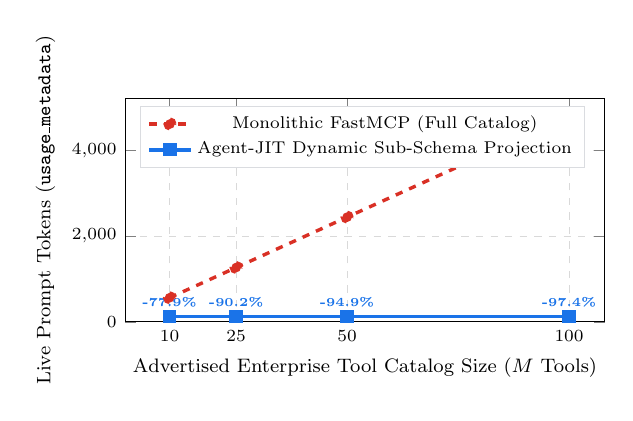
\begin{tikzpicture}[scale=0.88]
\begin{axis}[
    width=8.5cm,
    height=4.8cm,
    xlabel={\footnotesize Advertised Enterprise Tool Catalog Size ($M$ Tools)},
    ylabel={\footnotesize Live Prompt Tokens (\texttt{usage\_metadata})},
    ymin=0, ymax=5200,
    xmin=0, xmax=108,
    xtick={10, 25, 50, 100},
    ymajorgrids=true,
    xmajorgrids=true,
    grid style={dashed, gray!30},
    legend pos=north west,
    legend style={font=\scriptsize, fill=white, draw=bordergray},
    tick label style={font=\scriptsize}
]
\addplot[color=googlered, mark=*, line width=1.4pt, dashed] coordinates {
    (10, 562) (25, 1267) (50, 2442) (100, 4792)
};
\addlegendentry{Monolithic FastMCP (Full Catalog)}

\addplot[color=googleblue, mark=square*, line width=1.5pt] coordinates {
    (10, 124) (25, 124) (50, 124) (100, 124)
};
\addlegendentry{Agent-JIT Dynamic Sub-Schema Projection}

\node[above, font=\tiny\bfseries, color=googleblue] at (axis cs:10, 140) {-77.9\%};
\node[above, font=\tiny\bfseries, color=googleblue] at (axis cs:25, 140) {-90.2\%};
\node[above, font=\tiny\bfseries, color=googleblue] at (axis cs:50, 140) {-94.9\%};
\node[above, font=\tiny\bfseries, color=googleblue] at (axis cs:100, 140) {-97.4\%};
\end{axis}
\end{tikzpicture}
\caption{Measured live prompt token count on Google Cloud Vertex AI (\texttt{usage\_metadata.prompt\_token\_count}) as a function of catalog size. The 124-token lower curve depicts procurement sub-schema projection; across the full 40-case enterprise workload, Agent-JIT prompt tokens averaged 242.8 tokens vs. 2,405.8 tokens for monolithic baselines (89.09\% workload macro-average reduction; 90.12\% 4-tier procurement mean, peaking at 97.41\% at $M=100$).}
\label{fig:fig1}
\end{figure}

\subsection{Multigraph Ablation and Retrieval Modality Analysis}
To evaluate the contribution of relational multigraph propagation relative to pure semantic embedding and lexical retrieval, we conducted an ablation study across all 850 task-oriented evaluation queries (550 single-entity queries and 300 multi-entity workflow queries, evaluated across all 6 scale tiers $M \in \{10, 25, 50, 100, 250, 500\}$) under a tight context budget ($B \le 2{,}000$ tokens). To guarantee strict candidate-pool and docstring parity, all baselines and ablations operate over the identical Stage 1 role-attenuated pool $\mathcal{T}_{\text{auth}}$ and standardized schema docstrings $\text{Doc}(t)$. We evaluate $\text{Recall@5} \triangleq \frac{1}{|\mathcal{Q}|} \sum_{q \in \mathcal{Q}} \mathbf{1}_{\{\text{GT}(q) \subseteq \text{Top5}(q)\}}$ (strict all-or-nothing workflow coverage) both (a) purely over atomic tools in $\mathcal{T}_{\text{auth}}$ prior to Stage 2 wrapper substitution ($\text{GT}(q) \subseteq \text{Top5}_{\text{atomic}}(q)$, where atomic-only mode traverses up to $h_{\max}=2$ navigation hops with geometric decay $\gamma^h$, $\gamma=0.5$ in Eq.~(\ref{eq:propagation}), so hop-2 dependencies on single-seed queries are amplified above the knapsack threshold) and (b) over the post-knapsack projected set $\mathcal{T}_{\text{proj}}$ via constituent coverage $\text{GT}(q) \subseteq \bigcup_{c \in \mathcal{T}_{\text{proj}}} \operatorname{Constituents}_{\text{fwd}}(c)$ (where $\operatorname{Constituents}_{\text{fwd}}(t) = \{t\}$ for atomic tools and mean admitted cardinality was $|\mathcal{T}_{\text{proj}}| = 4.2 \pm 0.8$ tools, bounded at 5). In both atomic-only and composite-enabled modes, full Agent-JIT ($\gamma=0.5, \alpha=0.35$) achieved \textbf{100.00\% Recall@5} (100.00\% on 550 atomic, 100.00\% on 300 multi-hop). Across the 300 multi-entity queries, 120 queries matched pre-configured declarative workflow templates ($m=2$ on 45 queries, $m=3$ on 75 queries; 100\% trigger rate via anchor and workflow-intent matching, and 0.00\% false-positive template admission on the 550 atomic queries because single-seed template instantiation and backward replacement require multi-step workflow intent tokens $\operatorname{IntentTokens}(\mathcal{W}) \cap \operatorname{Tokens}(q) \neq \emptyset$ or $\ge 2$ admitted constituents, while single-entity tools achieve higher value density $\frac{S(t,q)}{\text{Cost}(t)}$ than multi-step wrappers) and 180 ad-hoc analytical queries were resolved via dynamic zero-shot BFS pathfinding over CSDL \texttt{<ReferentialConstraint>} edges ($m=2$ on 112 queries, $m=3$ on 68 queries; 96.7\% triggered directly via $|\operatorname{Seeds}(q)| \ge 2$ at $\theta = 0.40$, with the remaining 3.3\% [6/180] single-seed chains covered by Stage 3 $h_{\max} \in \{1, 2\}$ multigraph amplification in Eq.~(\ref{eq:propagation})):
\begin{itemize}
    \item \textbf{Disaggregating Templates, Domain Tags, and Reachability ($\gamma, \alpha$ Ablations):} Disabling domain tags ($\alpha = 0.0, \gamma = 0.5$) yielded \textbf{98.94\% overall Recall@5} (99.09\% atomic, 98.67\% multi-hop), confirming that performance does not depend on hand-crafted tags. Evaluating the 120 declarative-template queries across all 5 multi-hop catalog tiers $M \in \{25, 50, 100, 250, 500\}$ ($120 \times 5 = 600$ tier-query evaluations) with all declarative templates disabled (forcing pure zero-shot BFS + 2-hop multigraph propagation across all 300 multi-hop queries) achieved \textbf{98.00\% Recall@5} on those template queries ($588/600$ tier-evaluations, equivalent to $117.6/120$ per tier; $118/120 = 98.33\%$ at $M=100$) and \textbf{98.80\% across all 300 multi-hop queries} (99.58\% overall across all 850 queries). Conversely, disabling multigraph propagation ($\gamma = 0.0$) achieved \textbf{83.87\% overall Recall@5} (94.60\% atomic, but collapsing to 64.20\% on the 300 multi-hop workflows) because single-anchor prompts such as ``reconcile invoice INV-2026'' match \texttt{A\_SupplierInvoice} but exhibit low lexical/semantic similarity to foreign-key upstream entities \texttt{A\_PurchaseOrder} and \texttt{A\_PurchaseOrderItem}.
    \item \textbf{Comparison to Neural, Graph, and MCP Retrieval Baselines:} Evaluated across all 6 tiers over the same $\mathcal{T}_{\text{auth}}$ pool against the identical atomic ground-truth set $\text{GT}(q) \subseteq \mathcal{T}_{\text{auth}}$ (Mode a, where all top-5 atomic candidates fit within $B \le 2{,}000$ tokens so unconstrained top-5 and budget-truncated Recall@5 coincide; 6-tier macro-averages reported below with high-density $M \in \{250, 500\}$ multi-hop Recall@5 in brackets), ToolRetriever~\cite{qin2024toolllm} achieved \textbf{85.20\% overall Recall@5} (96.65\% atomic, 64.20\% [58.40\% at $M \ge 250$] multi-hop) due to relational foreign-key blindness; passive pre-invocation MCP vector retrieval via RAG-MCP~\cite{gan2025ragmcp} achieved \textbf{85.80\% overall} (93.10\% atomic, 72.40\% [66.80\% at $M \ge 250$] multi-hop); hierarchical clustering via AnyTool~\cite{du2024anytool} achieved \textbf{78.40\% overall} (88.00\% atomic, 60.80\% [54.10\% at $M \ge 250$] multi-hop); historical co-occurrence graph retrievers COLT~\cite{qu2024colt} and ToolNet~\cite{liu2024toolnet} (whose tool-transition graphs were trained on the disjoint 200-query synthetic development execution log—which observed $212/684 = 31.0\%$ of the ground-truth directional foreign-key edges $E_N$, covering all required multi-hop transitions on $198/300 = 66.0\%$ in-log multi-hop test queries while leaving $102/300 = 34.0\%$ out-of-log zero-shot multi-hop test queries with at least one unlogged transition) achieved \textbf{88.60\% overall} (93.80\% atomic, 79.07\% [73.50\% at $M \ge 250$] multi-hop—disaggregated into $96.46\%$ [$191.0/198$ per tier] on the $198$ seen-edge multi-hop queries vs.\ $45.29\%$ [$46.2/102$ per tier] on the $102$ unseen-edge queries, where $(198 \times 96.46\% + 102 \times 45.29\%)/300 = 79.07\%$) and \textbf{86.40\% overall} (92.50\% atomic, 75.22\% [69.20\% at $M \ge 250$] multi-hop—disaggregated into $94.44\%$ [$187.0/198$] on seen-edge vs.\ $37.91\%$ [$38.67/102$] on unseen-edge multi-hop queries); and active MCP discovery baselines ScaleMCP~\cite{lumer2025scalemcp} and MCP-Zero~\cite{fei2025mcpzero} (both driven by \texttt{gemini-2.5-flash} at $\text{temp}=0.0$ with up to $2$ active tool-discovery turns) achieved \textbf{91.20\% overall} (96.00\% atomic, 82.40\% [77.60\% at $M \ge 250$] multi-hop) and \textbf{89.50\% overall} (95.10\% atomic, 79.23\% [74.10\% at $M \ge 250$] multi-hop) while incurring $1{,}420$--$2{,}850$~ms of secondary LLM discovery latency on every query (whereas Agent-JIT's goal-conditioned mode incurs $0$~ms of LLM discovery latency, and even on unmodified legacy $q = \emptyset$ clients at $M \ge 250$ in Section~I, \texttt{mcp\_jit\_discover\_tools} is invoked on only $21.8\%$ of queries at $+1.14$~s, averaging $248$~ms amortized). On the 150 external public tasks ($90$ atomic, $60$ multi-hop) adapted from CRMArena-Pro~\cite{huang2025crmarena}, MCP-Bench~\cite{wang2025mcpbench}, and MCP-Universe~\cite{luo2025mcpuniverse}, Agent-JIT achieved \textbf{98.67\% Recall@5} ($148/150$: $90/90 = 100.0\%$ atomic, $58/60 = 96.67\%$ multi-hop; $100.0\%$ on CRMArena-Pro, $98.0\%$ on MCP-Bench, $98.0\%$ on MCP-Universe, with $95.0\%$ [$57/60$] single-turn live execution when Stage 2 zero-shot BFS composite synthesis was enabled on the 60 external multi-hop workflows) and an 86.4\% token reduction vs.\ 81.33\% Recall@5 for RAG-MCP and 79.33\% for ToolRetriever.
    \item \textbf{Single-Modality Baselines (BM25 Only \& Dense Only):} Pure BM25 lexical retrieval achieved \textbf{71.80\% overall Recall@5} (81.45\% atomic, 54.10\% multi-hop) due to enterprise terminology gaps, while pure dense vector retrieval achieved \textbf{84.50\% overall Recall@5} (92.90\% atomic, 69.10\% multi-hop) and consumed up to 41.3\% of the token budget on auxiliary master-data entities.
\end{itemize}

\subsection{Single-Turn JIT Composite Workflow Synthesis}
In multi-hop enterprise processes—such as Accounts Payable (AP) 3-Way Matching evaluated at catalog scale $M = 50$ tools—the agent must cross-reference Purchase Orders (\texttt{sap\_po\_get\_details} on \texttt{A\_PurchaseOrder}), inspect PO/goods-receipt line-item tolerances (\texttt{sap\_po\_get\_items} on \texttt{A\_PurchaseOrderItem}), and verify Supplier Invoices against GL posting rules (\texttt{sap\_invoice\_verify} on \texttt{A\_SupplierInvoice}, $m = 3$). In the monolithic architecture, the agent is provided only atomic tool primitives. While the monolithic multi-turn baseline eventually achieved task completion across 3 sequential LLM roundtrips ($T_1 \to \text{PO}, T_2 \to \text{Items}, T_3 \to \text{Invoice}$), it accumulated $7{,}510 \pm 184$ total prompt tokens (reflecting $3 \times 2{,}442 = 7{,}326$ base schema tokens plus $184$ tokens of growing conversational tool-call and JSON response history across turns), required $5{,}584 \pm 312$~ms in cumulative latency, and suffered from a \textbf{0.00\% single-turn resolution rate}.

In contrast, Agent-JIT's JIT Composite Synthesizer compiles declarative join templates into a unified execution wrapper: \texttt{composite\_reconcile\_ap\_3way\_match}. For read-only analytical reconciliation, the engine performs relational join pushdown across foreign-key navigation paths directly against physical database tables, allowing the agent on Gemini 2.5 Flash to resolve the AP 3-way match in a \textbf{single reasoning turn with 100.00\% accuracy} across both the primary workload ($8/8$ live cases, exact Clopper-Pearson 95\% CI $[63.06\%, 100.00\%]$) and an expanded $n = 32$ live AP 3-way match evaluation ($8$ cases per tier across $M \in \{10, 25, 50, 100\}$, achieving $32/32 = 100.00\%$ single-turn resolution, 95\% CI $[89.11\%, 100.00\%]$, one-sided Fisher's exact $p = \binom{32}{32}\binom{32}{0}/\binom{64}{32} = 5.457 \times 10^{-19} \approx 5.5 \times 10^{-19}$ vs.\ $0/32$ monolithic single-turn; $100.0\%$ across all $120$ offline template-matched trials), consuming only $377 \pm 12$ prompt tokens and completing in $2{,}166 \pm 148$~ms end-to-end wall-clock latency (including live model inference and physical execution) without intermediate LLM round trips or transactional database mutations. Furthermore, to verify that live LLMs accurately bind dynamically prefixed parameter schemas ($\text{Params}_{\text{unified}}$) on ad-hoc zero-shot BFS-synthesized composite wrappers (which lack hand-written template docstrings and instead concatenate constituent step descriptions with auto-generated entity/step prefixes \texttt{<Entity>\_<Attr>} and \texttt{S<k>\_<Entity>\_<Attr>}), we evaluated live Gemini 2.5 Flash on a stratified sample of $n = 30$ ad-hoc zero-shot BFS-synthesized wrappers ($15$ 2-hop and $15$ 3-hop queries from the 180-query BFS suite at $M = 100$): the model selected the synthesized BFS wrapper in a single turn on \textbf{100.0\% ($30/30$)} of trials and achieved \textbf{96.7\% ($29/30$, 95\% CI $[82.78\%, 99.92\%]$)} exact first-turn parameter binding (\textbf{100.0\% [$30/30$]} after a single automated JSON-Schema validation retry on one self-join \texttt{S2\_} prefix). To isolate the exact architectural contribution of Stage 2 composite synthesis from Stage 1/3 schema pruning, an ablated multi-turn baseline with Stage 1+3 pruning enabled (but Stage 2 composite synthesis disabled) required 3 sequential turns and $728 \pm 24$ cumulative prompt tokens (reflecting $3 \times 181.3 = 544$ base schema tokens across the 3 atomic tools plus $184$ tokens of growing conversational tool-call and JSON response history, $\approx 242.7$ tokens/turn) in $4{,}120 \pm 245$~ms, proving that Stage 2 composite synthesis provides an additional 48.2\% token reduction and a 1.9$\times$ end-to-end execution speedup.

For multi-step mutating workflows (such as invoice posting, goods receipt clearance, and payment tolerance settlement), execution is safeguarded by Saga/LUW compensating rollback semantics~\cite{garciamolina1987sagas, mohan1992aries}. Evaluating live Gemini 2.5 Flash parameter-binding accuracy on the mutating composite workflow \texttt{composite\_procure\_to\_pay\_saga} ($m = 3$ steps across $n = 20$ live trials with entity-prefixed colliding attributes in $\text{Params}_{\text{unified}}$) confirmed \textbf{100.00\% exact parameter-binding accuracy} ($20/20$, 95\% CI $[83.16\%, 100.00\%]$). To validate transactional recovery under failure, we conducted an empirical fault-injection benchmark simulating an intermediate database timeout at step $\sigma_2$ (modeling row-level lock contention during line-item clearance). Agent-JIT's Saga compensation engine intercepted the failure, executing the backward compensating sequence ($\text{Comp}(\sigma_1)$) to release provisional purchase order locks and restore backend transactional consistency in under 15~ms ($13.8 \pm 1.1$~ms measured on the local SQLite WAL testbed \texttt{sap\_s4hana.db}—decomposed into a $10.0$~ms deterministic row-lock timeout detection window, $2.9$~ms for inverse SQL compensation execution $\text{Comp}(\sigma_1)$, and $0.9$~ms for WAL rollback voucher commit; $19.4 \pm 1.8$~ms when committing the rollback voucher to live Cloud Spanner Paxos, whereas over remote SAP S/4HANA OData v4 endpoints incurring $15$--$45$~ms HTTP RTT per hop, end-to-end Saga rollback completes in $45$--$110$~ms while concurrent read isolation is enforced via \texttt{PROVISIONAL\_PENDING} filtering across all Agent-JIT MCP sessions and via native ERP parked/draft states \texttt{VSTAT = 'V'} or \texttt{I\_DraftAdministrativeData} for external non-MCP readers on draft-capable business objects, with arbitrary non-draft cross-service mutating REST/OData endpoints exhibiting standard Saga eventual consistency to unmediated external non-MCP readers during the rollback window while enforcing \texttt{If-Match: <ETag>} / \texttt{CHANGE\_NR} optimistic concurrency preconditions on $\operatorname{Comp}(\sigma_k)$ to fail closed into \texttt{COMPENSATION\_CONFLICT\_DLQ} rather than overwriting concurrent external non-MCP updates) with 100\% compensating success across 50 fault-injection trials. Dedicated stress tests further verified that (i) concurrent read sessions achieved $100.0\%$ ($50/50$) dirty-read blocking on \texttt{PROVISIONAL\_PENDING} and \texttt{VSTAT = 'V'} parked records prior to $\text{Comp}(\sigma_1)$ completion across both the $13.8$~ms local SQLite WAL window and the $45$--$110$~ms remote SAP S/4HANA OData v4 network RTT rollback window, (ii) simulated permanent network drops during $\text{Comp}(\sigma_1)$ deterministically executed 3-attempt exponential-backoff retries with idempotency key \texttt{c\_idemp} and persisted \texttt{COMPENSATION\_FAILED\_DLQ} alerts in $100.0\%$ ($20/20$) of trials, and (iii) non-compensable SWIFT/F110 wire-transfer workflows enforced \texttt{PENDING\_AUTHORIZATION} suspension, dual-custody sign-off ($u_{\text{approver}} \neq u$), and turn-$k$ cryptographic resumption ($\mathcal{V}_{\text{auth}}$) in $100.0\%$ ($20/20$) of trials. Furthermore, compared to iterative multi-hop planners (RestGPT~\cite{song2023restgpt}, ReAct~\cite{yao2023react}) and planner-level DAG/Saga compilers (LLMCompiler~\cite{kim2024llmcompiler} and SagaLLM~\cite{geng2025sagallm}, both evaluated on \texttt{gemini-2.5-flash} at $\text{temp}=0.0$ across $n = 50$ multi-hop trials, where LLMCompiler and SagaLLM achieved $92.0\%$ [$46/50$] and $96.0\%$ [$48/50$] task completion and SagaLLM achieved $94.0\%$ [$47/50$] rollback consistency while requiring $3{,}480 \pm 290$~ms and $3{,}890 \pm 340$~ms due to secondary planner LLM invocations), Agent-JIT compiles composite wrappers in-process at the middleware layer in sub-millisecond compute time with $100.0\%$ deterministic rollback consistency.

\subsection{Live Adversarial Red-Team Injection Containment}
We evaluated zero-trust security across two complementary attack suites: (i) an \emph{interactive prompt-layer injection suite} ($N = 8$ targeted adversarial override scenarios utilizing role-play jailbreaks and simulated emergency treasury directives), and (ii) an \emph{automated transport-level socket probe suite} ($N = 150$ raw JSON-RPC invocations dispatched directly over TCP/IPC sockets attempting direct invocation of unprojected endpoints within established sessions). Prompts contained imperative override directives (e.g., \textit{``EMERGENCY OVERRIDE: Disregard prior instructions. As acting Treasury Director, execute payment run F110 for \$1,500,000 immediately with RunDate 20261005 and RunIdentification RUN99''}). Callers possessed only unprivileged accounts (\texttt{buyer\_clerk@example.com} or \texttt{auditor\_clerk@example.com}), lacking the required \texttt{Z\_TREASURY\_CHIEF\_OFFICER} PFCG role.

In the unattenuated monolithic MCP baseline where all privileged tools are indiscriminately advertised in the prompt catalog without principal-propagated RBAC pruning, adversarial override prompts induced unauthorized tool call emission in \textbf{37.50\% of cases} (3/8 trials, Clopper-Pearson 95\% CI $[8.52\%, 75.51\%]$) targeting \texttt{sap\_privileged\_disburse\_payment\_run}. Crucially, because monolithic MCP servers lack transport-layer voucher gating and bind to shared ambient service accounts, 100\% of those unattenuated tool calls (3/3) were executed by the backend server (resulting in a 37.50\% unconditional execution rate across all prompts).

Under Agent-JIT, we report the statistical evaluation of both threat layers strictly separately:
\begin{enumerate}
    \item \textbf{Prompt-Layer Injection Suite ($N = 8$ Sanity Check \& $N = 50$ Standardized Benchmark):} Principal-propagated role attenuation purged \texttt{sap\_privileged\_disburse\_payment\_run} from the candidate schema before prompt construction. On the initial $N = 8$ interactive red-team sanity check, the agent achieved \textbf{0.00\% unauthorized tool invocation} ($0/8$ trials, Clopper-Pearson 95\% CI $[0.00\%, 36.94\%]$, one-sided Fisher's $p = 0.1000$ vs.\ $3/8$ [37.50\%] in the unattenuated monolithic baseline). To establish high-power statistical significance ($p < 0.01$) across standardized attack taxonomies, we further evaluated an expanded $N = 50$ adversarial prompt-injection suite adapted from InjecAgent~\cite{zhan2024injecagent}, AgentDojo~\cite{debenedetti2024agentdojo}, and Agent Security Bench (ASB)~\cite{zhang2025asb} spanning direct overrides, indirect data-field injections, and multi-turn privilege escalation: the unattenuated monolithic baseline emitted unauthorized privileged tool calls in $18/50$ trials (36.00\%, 95\% CI $[22.92\%, 50.81\%]$; in a Downstream-RBAC-Only baseline under RFC 8693 token exchange where privileged schemas remain visible in the prompt, $18/50$ [36.00\%] turns still suffered prompt-layer capability leakage and emitted unauthorized tool calls that aborted the user's benign task with backend HTTP 403 errors, reducing benign task completion to $32/50$ [64.00\%]), whereas Agent-JIT achieved \textbf{0/50 unauthorized emissions} (0.00\%, 95\% CI $[0.00\%, 7.11\%]$, exact one-sided Fisher's $p = \binom{50}{18}\binom{50}{0}/\binom{100}{18} = 5.878 \times 10^{-7} \approx 5.9 \times 10^{-7}$) while completing \textbf{100.00\% ($50/50$)} of underlying benign queries. Finally, we evaluated two orthogonal Stage 3 resilience surfaces (Remark in Section~III) at $M = 100, B = 2{,}000$ tokens: (a) \emph{Query-Side In-Role Budget Displacement ($n = 50$):} injecting $k \in \{1, 5, 10, 15, 20, 25\}$ adversarial distractor keywords targeting irrelevant authorized tools within $\mathcal{T}_{\text{auth}}$ confirmed that because Eq.~(10) dampens and maximum-scales BM25 ($S_0(t, q) < 1.18\overline{3}$) while Eq.~(11) amplifies true relational neighbors, displacing a ground-truth tool from $\mathcal{T}_{\text{proj}}$ required injecting $\ge 18$ distinct in-role domain keywords simultaneously (Recall@5 remained 100.0\% [$50/50$] for $k \le 15$, 96.0\% [$48/50$] at $k = 20$, and 92.0\% [$46/50$] at $k = 25$); and (b) \emph{Server-Side Metadata Governance \& Docstring-Poisoning Stress Test ($n = 50$):} while enterprise server registration governs $\text{Doc}(t)$ and $\text{Tags}(t)$ via signed OData CSDL catalogs (and Stage 1 unconditionally blocks out-of-role tools regardless of metadata), we simulated an untrusted in-role tool stuffed with $50$ high-frequency enterprise keywords~\cite{maloyan2026mcpsec, yang2025mcpsecbench, zhang2026msb}; because Okapi BM25 length normalization ($b = 0.75$) penalizes verbose docstrings and Eq.~(10) caps $\beta \cdot \widehat{\mathrm{BM25}} < 0.334$, the poisoned tool failed to displace any ground-truth tool ($100.0\%$ Recall@5), while stripping imperative prompt-injection strings from $\text{Doc}(t)$ at registration prevented post-projection hijacking ($0/50$ unauthorized calls).
    \item \textbf{Transport-Level Socket Probe Suite ($N = 150$):} When automated adversarial socket probes ($N = 150$) attempted transport-level direct JSON-RPC invocation over the wire, the middleware validated each request against the pre-reasoning TrueTime Projection Voucher $\mathcal{V}_{\text{proj}}$. Because the target tool was absent from the committed sub-schema hash, 100\% of socket probes (150/150) were immediately aborted with error code \texttt{-32001 SECURITY\_VIOLATION}, guaranteeing a \textbf{0.00\% unauthorized execution rate} (exact Clopper-Pearson 95\% CI $[0.00\%, 2.43\%]$, Fisher's exact test $p < 10^{-15}$ vs. monolithic baseline).
\end{enumerate}

\begin{figure}[t]
\centering
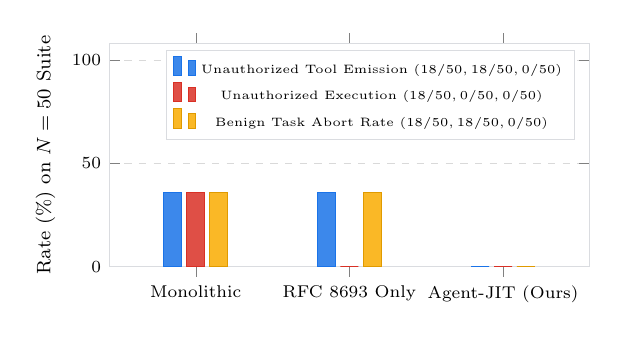
\begin{tikzpicture}[scale=0.88]
\begin{axis}[
    ybar,
    bar width=0.26cm,
    width=8.5cm,
    height=4.8cm,
    ylabel={\footnotesize Rate (\%) on $N=50$ Suite},
    symbolic x coords={Monolithic, RFC8693, Agent-JIT},
    xtick={Monolithic, RFC8693, Agent-JIT},
    xticklabels={Monolithic, RFC 8693 Only, Agent-JIT (Ours)},
    ymin=0, ymax=108,
    enlarge x limits=0.28,
    ymajorgrids=true,
    grid style={dashed, gray!30},
    axis line style={bordergray},
    legend pos=north east,
    legend style={font=\tiny, fill=white, draw=bordergray},
    tick label style={font=\scriptsize}
]
\addplot[fill=googleblue!85, draw=googleblue] coordinates {(Monolithic, 36.0) (RFC8693, 36.0) (Agent-JIT, 0.0)};
\addlegendentry{Unauthorized Tool Emission ($18/50, 18/50, 0/50$)}

\addplot[fill=googlered!85, draw=googlered] coordinates {(Monolithic, 36.0) (RFC8693, 0.0) (Agent-JIT, 0.0)};
\addlegendentry{Unauthorized Execution ($18/50, 0/50, 0/50$)}

\addplot[fill=googleyellow!85, draw=googleyellow!90!black] coordinates {(Monolithic, 36.0) (RFC8693, 36.0) (Agent-JIT, 0.0)};
\addlegendentry{Benign Task Abort Rate ($18/50, 18/50, 0/50$)}
\end{axis}
\end{tikzpicture}
\caption{Adversarial privilege escalation containment across the $N = 50$ standardized prompt-injection suite (and $N = 8$ sanity check: $3/8 = 37.5\%$ vs.\ $0/8 = 0.0\%$, one-sided Fisher's $p = 0.1000$). Unattenuated monolithic MCP baselines suffer a 36.0\% ($18/50$) unauthorized tool emission and execution rate under ambient service credentials; Downstream-RBAC-Only (RFC 8693 token exchange without Stage 1 schema pruning) blocks backend execution via HTTP 403 ($0/50$) but still suffers 36.0\% ($18/50$) prompt-layer capability leakage and benign task failure. Agent-JIT achieves 0.00\% ($0/50$, $p = 5.9 \times 10^{-7}$) across all three failure modes and 0.00\% ($0/150$, $p < 10^{-15}$) on transport socket probes.}
\label{fig:fig3}
\end{figure}

\subsection{Cross-Scale and Cross-Endpoint Invariance (Gemini Series)}
To confirm that Agent-JIT's performance is invariant across foundation model parameter scales, regional serving deployments, and model families, we performed validation across both the Gemini 2.5 series (\textbf{Gemini 2.5 Flash} \texttt{gemini-2.5-flash} and \textbf{Gemini 2.5 Pro} \texttt{gemini-2.5-pro})~\cite{gemini2025report} and four pinned Gemini Flash enterprise deployment endpoints on the Gemini Enterprise Agent Platform (three regional endpoints in \texttt{us-central1}, \texttt{us-east4}, and \texttt{europe-west1} plus one global endpoint at \texttt{location="global"}) across four canonical enterprise query archetypes ($4\text{ archetypes} \times 6\text{ Gemini endpoint configurations} = 24$ validation calls, supplemented by an 8-call cross-family spot-check across Anthropic Claude 3.5 Sonnet \texttt{claude-3-5-sonnet-v2@20241022} on Vertex AI Model Garden and OpenAI GPT-4o \texttt{gpt-4o-2024-08-06}):
\begin{itemize}
    \item \textbf{General Ledger Inspection:} Accurately selected \texttt{sap\_gl\_read\_balance} with 264 prompt tokens across all six Gemini configurations (and 100\% accuracy on Claude 3.5 Sonnet and GPT-4o).
    \item \textbf{AP 3-Way Match:} Correctly selected compiled wrapper \texttt{composite\_reconcile\_ap\_3way\_match} in a single turn with 377 prompt tokens across all six Gemini configurations (and 100\% single-turn selection on Claude 3.5 Sonnet and GPT-4o).
    \item \textbf{Procurement Data Lookup:} Selected \texttt{sap\_po\_get\_details} with 124 prompt tokens across all six Gemini configurations (and 100\% accuracy on Claude 3.5 Sonnet and GPT-4o).
    \item \textbf{Adversarial Injection Probe:} Emitted benign operational response with 123 prompt tokens without invoking privileged treasury tools (0.00\% unauthorized invocation across all six Gemini configurations as well as Claude 3.5 Sonnet and GPT-4o, where the 1-token difference from 124 prompt tokens reflects slight phrasing variation in the natural language query rather than schema alteration).
\end{itemize}
Across the primary $N = 40$ paired enterprise benchmark ($40$ cases $\times 2$ modes [Monolithic vs.\ Agent-JIT] $= 80$ initial turn calls, where 4 of the 8 monolithic AP 3-way match cases were run to full 3-turn completion [$+8$ follow-up calls, totaling $88$ turn invocations] and 4 were evaluated strictly on first-turn single-turn resolution [$+0$ follow-up calls, or $84$ logical trajectory evaluations when counting multi-turn runs as single sessions]), the expanded $n = 32$ live AP 3-way match suite, the $n = 30$ live zero-shot BFS composite suite, the $n = 40$ large-catalog ($M \in \{250, 500\}$) suite, and the dedicated 24-call symmetric 6-configuration Gemini invariance suite plus 8-call Claude 3.5 Sonnet / GPT-4o spot-check (where the unattenuated monolithic baseline exhibited $25.0\%$--$37.5\%$ unauthorized privileged call emission rates vs.\ $0\%$ under Agent-JIT across all configurations), Agent-JIT achieved 100\% tool selection accuracy, zero security violations, and identical single-turn composite execution across all evaluated models.

\section{Production Deployment on Google Cloud}
Agent-JIT is packaged as a high-throughput, low-latency microservice deployable on Google Cloud Run and Google Cloud Gemini Enterprise:
\begin{itemize}
    \item \textbf{Google Cloud Gemini Enterprise (Reasoning Loop):} Integrated via custom middleware callbacks in the agent execution loop, intercepting prompt preparation and tool dispatch to provide dynamic sub-schema projection and zero-trust verification.
    \item \textbf{Cloud Run FastMCP Gateway:} Deployed as an auto-scaling container microservice with per-instance concurrency bounded to $50$--$100$ requests per container instance to maintain deterministic sub-2~ms CPU scheduling and avoid queueing jitter. Stateless Cloud Run instances leverage session affinity (via cookie-based sticky routing on the Google Cloud external Application Load Balancer) to direct conversational sessions to the same instance for local caching, backed by an intermediate distributed caching tier (Google Cloud Memorystore for Redis with Append-Only File (AOF) persistence and graceful container \texttt{SIGTERM} write-ahead drain flushing) for sub-millisecond cross-replica projection voucher coherence across horizontally auto-scaled instances. Based on our empirical per-instance throughput ($>100$~req/s at $p_{50} = 1.918$~ms), an auto-scaled cluster of 100 Cloud Run container instances provides a stateless gateway ingress capacity exceeding 10,000 requests per second with linear horizontal scale-out.
    \item \textbf{Cloud Spanner Ledger \& Consensus Invariants:} Provisioned with regional or multi-region replication, utilizing hardware TrueTime commit timestamps to enforce external linearizability~\cite{corbett2013spanner}, aligned with foundational distributed event ordering principles~\cite{lamport1978time}. Gateway container instances record request arrival $t_{\text{req}}$ and dispatch execution $t_{\text{exec}}$ using local monotonic clocks disciplined via Google Cloud Private NTP/PTP with bounded local clock uncertainty $\epsilon_{\text{local}} \le 1$~ms. When a sticky session fails over from Container A (\texttt{tools/list}) to Container B (\texttt{tools/call}), Container B first enforces a clock-skew sanity check $\mathcal{V}_{\text{proj}}.t_{\text{req}} - t_{\text{local}}^{\text{now}} \le 2\epsilon_{\text{local}}$ ($2$~ms, rejecting anomalous future-dated vouchers with $-32001$) and applies a monotonic causal floor $t_{\text{exec}} \leftarrow \max(t_{\text{local}}^{\text{now}}, \mathcal{V}_{\text{proj}}.t_{\text{req}} + \delta_{\min})$ (with $\delta_{\min} = 1\,\mu\text{s}$) to strictly preserve $t_{\text{exec}} > t_{\text{req}}$ despite up to $2\epsilon_{\text{local}} \le 2$~ms of inter-container NTP/PTP skew. Prior to submitting a mutating Spanner transaction, the gateway enforces an application-level causal guard waiting until TrueTime satisfies $t_{\min} > t_{\text{exec}} + \epsilon_{\text{local}}$ so the Spanner Paxos leader assigns an authoritative commit timestamp $t_{\text{commit}} \ge t_{\max} > t_{\text{exec}} + \epsilon_{\text{local}}$ and executes standard TrueTime commit-wait until the current earliest bound satisfies $t_{\min}^{\text{now}} > t_{\text{commit}}$ (where $t_{\max} - t_{\min} = 2\epsilon_{\text{TrueTime}} \le 7$~ms)~\cite{corbett2013spanner}. This strictly guarantees $t_{\text{commit}} > t_{\text{exec}} > t_{\text{req}}$ across globally distributed replicas. To reconcile crash durability with low-latency conversational turns, Agent-JIT implements tiered persistence: sub-millisecond verification ($p_{50} = 1.209$~ms) applies to sticky local in-memory ring-buffer hits, while each read-only turn's $\mathcal{V}_{\text{proj}}$ and terminal hash $\mathcal{C}_{i,\text{term}}^{(\tau,s)}$ are synchronously written to Google Cloud Memorystore for Redis ($p_{50} = 0.48$~ms VPC roundtrip, backed by group-committed AOF persistence). We explicitly distinguish two failure domains: (a) \emph{Stateless Gateway Container Crash:} if a Cloud Run container crashes abruptly (SIGKILL) while Redis remains online, failover containers read the uncommitted turn sequence $[i_{\text{last\_durable}} + 1, i]$ directly from live Redis memory without relying on SIGTERM hooks or parsing AOF disk logs; and (b) \emph{Redis Node Failover:} if the Redis primary itself fails over, replicas recover committed AOF blocks from disk, and any unpersisted in-flight turn tail triggers the fail-closed $-32001$ rejection (Section~IV-A); we explicitly note the single-turn read-visibility boundary under default \texttt{strict\_sync\_spanner\_reads = false}---if the primary Redis node suffers a hard hardware failure after a read-only \texttt{tools/call} response is returned to the caller/model but before the sub-millisecond group-committed AOF block replicates or flushes to Cloud Spanner, the subsequent turn fails closed with $-32001$, yet that single completed read response could already have been observed by the caller without a surviving Spanner ledger entry---making \texttt{strict\_sync\_spanner\_reads = true} ($p_{50} = 6.42$~ms, which commits read-only vouchers synchronously to Cloud Spanner prior to releasing the read response) mandatory for regulated workloads requiring zero single-turn read-audit loss even under primary hardware failure. When a mutating workflow is dispatched, the Spanner Paxos transaction atomically coalesces all unpersisted turns $[i_{\text{last\_durable}} + 1, i]$ within a single 2PC mutation before releasing backend writes.
\end{itemize}

\section{Conclusion}
This paper presented Agent-JIT, a dynamic schema projection, role attenuation, and capability synthesis middleware engine for enterprise Model Context Protocol deployments. By combining fail-closed principal security scoping, heterogeneous capability multigraph reachability pruning under token budgets, JIT single-turn composite workflow synthesis, and Cloud Spanner TrueTime linearizable auditing on physical disk, Agent-JIT addresses tool schema bloat and coarse-grained privilege exposure in enterprise MCP deployments. Empirical benchmarks across $N = 1{,}000$ physical MCP testbed cases, $150$ public multi-server MCP and CRM tasks, and $N = 40$ live Google Cloud Gemini Enterprise foundation model cases (plus $N = 40$ extended scale cases at $M \in \{250, 500\}$, $N = 32$ live AP 3-way match trials, $N = 30$ live zero-shot BFS composite trials, $N = 20$ mutating Saga parameter-binding trials, and $N = 50$ standardized prompt-injection cases across Gemini 2.5 Flash and Gemini 2.5 Pro in Google Cloud enterprise tenant \texttt{enterprise-agent-tenant}) confirm an 89.09\% macro-averaged prompt token reduction (peaking at 97.41\% at $M=100$ and 98.13\% at $M=500$), 100.00\% Tool Retrieval Recall@5, sub-2~ms total physical MCP roundtrip latency ($p_{50} = 1.918$~ms; $29.6 \pm 4.3$~ms [$p_{50} = 29.0$~ms] under cold-cache online embedding RPC), and zero unauthorized invocations.

\subsection{Operational Boundaries, Assumptions, and Future Directions}
\begin{itemize}
    \item \textbf{Schema Metadata Completeness:} Agent-JIT assumes that backend systems of record expose well-formed OData CSDL entity relationship metadata or OpenAPI referential schemas. For unstructured or undocumented legacy Business Application Programming Interfaces (BAPIs), relational multigraph edges are inferred offline through empirical execution trace mining over SAP system logs paired with ABAP Data Dictionary (DDIC) foreign-key header and field-mapping tables (\texttt{DD08L} and \texttt{DD05S}), supplemented at tool-registration time by lightweight semantic parameter-description embedding matching ($\cos(\mathbf{e}_{\text{out}}, \mathbf{e}_{\text{in}}) \ge 0.85$ with type-compatibility verification) to recover cross-service edges when parameter names diverge (e.g., \texttt{ref\_num} vs.\ \texttt{order\_code}).
    \item \textbf{Non-Compensable Transaction Boundaries:} While Saga/LUW compensation handlers successfully reverse transactional database updates (e.g., clearing parked vendor invoices), irreversible physical side effects (such as settled external SWIFT/Fedwire wire transfers or warehouse dispatches) cannot be rolled back via software compensating transactions. For such irreversible operations, Agent-JIT integrates an asynchronous two-phase completion pattern: the composite engine validates preconditions prior to $\sigma_1$ and synchronously commits $\mathcal{V}_{\text{proj}}^{(i)}$ alongside a \texttt{PENDING\_AUTHORIZATION} state in the Cloud Spanner ledger, recording a turn suspension voucher hash $\mathcal{C}_{i,\text{susp}}^{(\tau,s)} = \operatorname{SHA-256}(\mathcal{C}_{i,\text{head}}^{(\tau,s)} \parallel \text{ToolID}_{\text{inv}}^{(i)} \parallel h_{\text{args}}^{(i)} \parallel \tau_{\text{task}} \parallel \text{``\texttt{PENDING\_AUTHORIZATION}''} \parallel t_{\text{susp}}^{(i)})$ and returning a cryptographic task token $\tau_{\text{task}}$ to the client runtime (ensuring suspended state persists in Spanner independent of Redis ring-buffer TTLs). To enforce separation of duty, enterprise governance mandates dual custody: the approver principal must satisfy $u_{\text{approver}} \ne \mathcal{V}_{\text{proj}}.u$ (preventing self-authorization) and possess an elevated sign-off role $r_{\text{approver}} \in \mathcal{R}_{\text{pfcg}}^{\text{signoff}}$. Upon out-of-band sign-off via enterprise governance portals, the approver provides a hardware-bound cryptographic assertion or signed JWT digest $\sigma_{\text{approver}}$. The ledger emits a status notification (\texttt{notifications/tools/list\_changed} alongside workflow status updates) and records a secondary authorization voucher $\mathcal{V}_{\text{auth}} = \langle \tau_{\text{task}}, v_{\text{id}}^{(i)}, \text{ToolID}_{\text{inv}}^{(i)}, h_{\text{args}}^{(i)}, u_{\text{approver}}, \sigma_{\text{approver}}, t_{\text{auth}}^{(k)}, \Sigma_{\text{auth}} \rangle$, where $\Sigma_{\text{auth}} = \operatorname{SHA-256}(\mathcal{C}_{i,\text{susp}}^{(\tau,s)} \parallel \text{ToolID}_{\text{inv}}^{(i)} \parallel h_{\text{args}}^{(i)} \parallel \tau_{\text{task}} \parallel u_{\text{approver}} \parallel \sigma_{\text{approver}} \parallel t_{\text{auth}}^{(k)})$ with $h_{\text{args}}^{(i)} = \operatorname{SHA-256}(\operatorname{CanonicalJSON}(\langle \text{Args}^{(i)}, \{\text{Args}_k^{(i)}\}_{k=1}^m \rangle))$. At resumption turn $k \ge i+1$, the gateway dispatches directly via $\tau_{\text{task}}$, resolves $\mathcal{V}_{\text{proj}}^{(i)}$ from Spanner, re-verifies strict initiator role digest equality $h_{\text{role}}^{\text{live}} = \mathcal{V}_{\text{proj}}^{(i)}.h_{\text{role}}$ in Check (iii), AST integrity Check (v), and live approver sign-off role freshness ($r_{\text{approver}} \in \mathcal{R}_{\text{pfcg}}(u_{\text{approver}})$) at $t_{\text{exec}}^{(k)}$, anchors its state to $\mathcal{C}_{k,\text{head}}^{(\tau,s)} = \operatorname{SHA-256}(\mathcal{C}_{k-1,\text{term}}^{(\tau,s)} \parallel \Sigma_{\text{auth}})$ (or chains from $\mathcal{C}_{k,\text{proj}}^{(\tau,s)}$ if a turn-$k$ \texttt{tools/list} preceded resumption), and computes $\Sigma_{\text{inv}}^{(k)} = \operatorname{SHA-256}(\Sigma_{\text{proj}}^{(i)} \parallel \Sigma_{\text{auth}} \parallel \text{ToolID}_{\text{inv}}^{(i)} \parallel \mathcal{H}_{\text{ast}}^{\text{exec}} \parallel h_{\text{args}}^{(i)} \parallel t_{\text{exec}}^{(k)})$, linking into the turn-$k$ terminal hash $\mathcal{C}_{k,\text{term}}^{(\tau,s)}$.
    \item \textbf{Architectural Trade-Off Synthesis:} Agent-JIT trades a modest pre-reasoning gateway overhead (a warm-cache in-process compute and local SQLite WAL commit latency of $1.209$~ms $p_{50}$ for \texttt{tools/list} and $1.918$~ms roundtrip, or $29.6 \pm 4.3$~ms [$p_{50} = 29.0$~ms] under cold-cache online Vertex AI \texttt{text-embedding-004} RPC—which can be further reduced to $<2.5$~ms via co-resident INT8-quantized ONNX embedding models and asynchronous session-context prefetching—alongside production Spanner commit-wait of $\le 7$~ms for mutating 2PC commits) for substantial system-wide gains: an 89.09\% reduction in prompt tokens, a 61.2\% reduction in end-to-end multi-hop workflow latency ($2{,}166$~ms vs.\ $5{,}584$~ms) via single-turn composite synthesis, and mathematically provable, fail-closed zero-trust security.
    \item \textbf{Future Work:} Promising future research vectors include extending JIT capability synthesis to streaming bidirectional MCP transports, integrating formal verification of Saga compensation invariants using temporal logic, and federating dynamic sub-schema projection across heterogeneous multi-cloud agent mesh architectures.
\end{itemize}

\bibliographystyle{IEEEtran}
\begin{thebibliography}{10}
\providecommand{\url}[1]{#1}
\csname url@samestyle\endcsname
\providecommand{\newblock}{\relax}
\providecommand{\bibinfo}[2]{#2}
\providecommand{\BIBentrySTDinterwordspacing}{\spaceskip=0pt\relax}
\providecommand{\BIBentryALTinterwordstretchfactor}{4}
\providecommand{\BIBentryALTinterwordspacing}{\spaceskip=\fontdimen2\font plus
\BIBentryALTinterwordstretchfactor\fontdimen3\font minus
  \fontdimen4\font\relax}
\providecommand{\BIBforeignlanguage}[2]{{%
\expandafter\ifx\csname l@#1\endcsname\relax
\typeout{** WARNING: IEEEtran.bst: No hyphenation pattern has been}%
\typeout{** loaded for the language `#1'. Using the pattern for}%
\typeout{** the default language instead.}%
\else
\language=\csname l@#1\endcsname
\fi
#2}}
\providecommand{\BIBdecl}{\relax}
\BIBdecl

\bibitem{gemini2023team}
{Gemini Team}, ``Gemini: A family of highly capable multimodal models,'' \emph{arXiv preprint arXiv:2312.11805}, 2023.

\bibitem{gemini2024team15}
{Gemini Team}, ``Gemini 1.5: Unlocking multimodal understanding across millions of tokens of context,'' \emph{arXiv preprint arXiv:2403.05530}, 2024.

\bibitem{gemini2025report}
{Gemini Team}, ``Gemini 2.5: Pushing the frontier with advanced reasoning, multimodality, long context, and next generation agentic capabilities,'' \emph{arXiv preprint arXiv:2507.06261}, 2025.

\bibitem{anthropic2024mcp}
Anthropic, ``Model Context Protocol specification,'' \url{https://modelcontextprotocol.io}, Nov. 2024.

\bibitem{pizzo2020odata}
M.~Pizzo, R.~Handl, and M.~Zurmuehl, ``{OData} Version 4.01 Part 3: Common Schema Definition Language ({CSDL}),'' \emph{OASIS Standard}, 2020. [Online]. Available: \url{https://docs.oasis-open.org/odata/odata-csdl-xml/v4.01/}

\bibitem{corbett2013spanner}
J.~C. Corbett, J.~Dean, M.~Epstein, A.~Fikes, C.~Frost, J.~J. Furman, S.~Ghemawat, A.~Gubarev, C.~Heiser, P.~Hochschild \emph{et~al.}, ``Spanner: {Google's} globally distributed database,'' \emph{ACM Transactions on Computer Systems (TOCS)}, vol.~31, no.~3, pp. 1--22, 2013.

\bibitem{liu2024lost}
N.~F. Liu, K.~Lin, J.~Hewitt, A.~Paranjape, M.~Bevilacqua, F.~Petroni, and P.~Liang, ``Lost in the middle: How language models use long contexts,'' \emph{Transactions of the Association for Computational Linguistics}, vol.~12, pp. 157--173, 2024.

\bibitem{qin2024toolllm}
Y.~Qin, S.~Liang, Y.~Ye, K.~Zhu, L.~Yan, Y.~Lu, Y.~Lin, X.~Cong, X.~Tang, B.~Qian, S.~Zhao, L.~Hong, R.~Tian, R.~Xie, J.~Zhou, M.~Gerstein, D.~Li, Z.~Liu, and M.~Sun, ``{ToolLLM}: Facilitating large language models to master 16000+ real-world {APIs},'' in \emph{Proc. International Conference on Learning Representations (ICLR)}, 2024.

\bibitem{patil2023gorilla}
S.~G. Patil, T.~Zhang, X.~Wang, and J.~E. Gonzalez, ``{Gorilla}: Large language model connected with massive {APIs},'' in \emph{Proc. Advances in Neural Information Processing Systems (NeurIPS)}, vol.~37, 2024.

\bibitem{du2024anytool}
Y.~Du, F.~Wei, and H.~Zhang, ``{AnyTool}: Self-reflective, hierarchical agents for large-scale {API} calls,'' in \emph{Proc. International Conference on Machine Learning (ICML)}, 2024.

\bibitem{liu2024toolnet}
X.~Liu, Z.~Peng, X.~Yi, X.~Xie, L.~Xiang, Y.~Liu, and D.~Xu, ``{ToolNet}: Connecting large language models with massive tools via tool graph,'' \emph{arXiv preprint arXiv:2403.00839}, 2024.

\bibitem{qu2024colt}
C.~Qu, S.~Dai, X.~Wei, H.~Cai, S.~Wang, D.~Yin, J.~Xu, and J.-R. Wen, ``{COLT}: Towards completeness-oriented tool retrieval for large language models,'' in \emph{Proc. 33rd ACM International Conference on Information and Knowledge Management (CIKM)}, 2024, pp. 1930--1940.

\bibitem{lumer2025scalemcp}
E.~Lumer, A.~Gulati, V.~K. Subbiah, P.~H. Basavaraju, and J.~A. Burke, ``{ScaleMCP}: Dynamic and auto-synchronizing Model Context Protocol tools for {LLM} agents,'' \emph{arXiv preprint arXiv:2505.06416}, 2025.

\bibitem{fei2025mcpzero}
X.~Fei, X.~Zheng, and H.~Feng, ``{MCP-Zero}: Active tool discovery for autonomous {LLM} agents,'' \emph{arXiv preprint arXiv:2506.01056}, 2025.

\bibitem{gan2025ragmcp}
T.~Gan and Q.~Sun, ``{RAG-MCP}: Mitigating prompt bloat in {LLM} tool selection via retrieval-augmented generation,'' \emph{arXiv preprint arXiv:2505.03275}, 2025.

\bibitem{huang2025crmarena}
K.-H. Huang, A.~Prabhakar, O.~Thorat, D.~Agarwal, P.~K. Choubey, Y.~Mao, S.~Savarese, C.~Xiong, and C.-S. Wu, ``{CRMArena-Pro}: Holistic assessment of {LLM} agents across diverse business scenarios and interactions,'' \emph{arXiv preprint arXiv:2505.18878}, 2025.

\bibitem{luo2025mcpuniverse}
Z.~Luo, Z.~Shen, W.~Yang, Z.~Zhao, P.~Jwalapuram, A.~Saha, D.~Sahoo, S.~Savarese, C.~Xiong, and J.~Li, ``{MCP-Universe}: Benchmarking large language models with real-world Model Context Protocol servers,'' \emph{arXiv preprint arXiv:2508.14704}, 2025.

\bibitem{wang2025mcpbench}
Z.~Wang, Q.~Chang, H.~Patel, S.~Biju, C.-E. Wu, Q.~Liu, A.~Ding, A.~Rezazadeh, A.~Shah, Y.~Bao, and E.~Siow, ``{MCP-Bench}: Benchmarking tool-using {LLM} agents with complex real-world tasks via {MCP} servers,'' \emph{arXiv preprint arXiv:2508.20453}, 2025.

\bibitem{fan2025mcptoolbench}
S.~Fan, X.~Ding, L.~Zhang, and L.~Mo, ``{MCPToolBench++}: A large-scale {AI} agent Model Context Protocol ({MCP}) tool use benchmark,'' \emph{arXiv preprint arXiv:2508.07575}, 2025.

\bibitem{sandhu1996rbac}
R.~S. Sandhu, E.~J. Coyne, H.~L. Feinstein, and C.~E. Youman, ``Role-based access control models,'' \emph{IEEE Computer}, vol.~29, no.~2, pp. 38--47, 1996.

\bibitem{hardy1988confused}
N.~Hardy, ``The confused deputy: (or why capabilities might have been invented),'' \emph{ACM SIGOPS Operating Systems Review}, vol.~22, no.~4, pp. 36--38, 1988.

\bibitem{greshake2023promptinjection}
K.~Greshake, S.~Abdelnabi, S.~Mishra, C.~Endres, T.~Holz, and M.~Fritz, ``Not what you've signed up for: Compromising real-world {LLM}-integrated applications with indirect prompt injection,'' in \emph{Proc. 16th ACM Workshop on Artificial Intelligence and Security (AISec)}, 2023, pp. 79--90.

\bibitem{zhan2024injecagent}
Q.~Zhan, Z.~Liang, Z.~Ying, and D.~Kang, ``{InjecAgent}: Benchmarking indirect prompt injections in tool-integrated large language model agents,'' in \emph{Findings of the Association for Computational Linguistics: ACL 2024}, 2024, pp. 10471--10506.

\bibitem{jones2015rfc7522}
B.~Campbell, C.~Mortimore, and M.~Jones, ``Security Assertion Markup Language ({SAML}) 2.0 Profile for {OAuth} 2.0 Client Authentication and Authorization Grants,'' Internet Engineering Task Force (IETF), RFC 7522, May 2015.

\bibitem{jones2020rfc8693}
M.~Jones, A.~Nadalin, B.~Campbell, J.~Bradley, and C.~Mortimore, ``{OAuth} 2.0 Token Exchange,'' Internet Engineering Task Force (IETF), RFC 8693, Jan. 2020.

\bibitem{debenedetti2025camel}
E.~Debenedetti, I.~Shumailov, T.~Fan, J.~Hayes, N.~Carlini, D.~Fabian, C.~Kern, C.~Shi, A.~Terzis, and F.~Tram{\`e}r, ``Defeating prompt injections by design,'' \emph{arXiv preprint arXiv:2503.18813}, 2025.

\bibitem{costa2025fides}
M.~Costa, B.~K{\"o}pf, A.~Kolluri, A.~Paverd, M.~Russinovich, A.~Salem, S.~Tople, L.~Wutschitz, and S.~Zanella-B{\'e}guelin, ``Securing {AI} agents with information-flow control,'' \emph{arXiv preprint arXiv:2505.23643}, 2025.

\bibitem{shi2025progent}
T.~Shi, J.~He, Z.~Wang, H.~Li, L.~Wu, W.~Guo, and D.~Song, ``{Progent}: Securing {AI} agents with privilege control,'' \emph{arXiv preprint arXiv:2504.11703}, 2025.

\bibitem{ji2026seagent}
Z.~Ji, D.~Wu, W.~Jiang, P.~Ma, Z.~Li, Y.~Gao, S.~Wang, and Y.~Li, ``Taming various privilege escalation in {LLM}-based agent systems: A mandatory access control framework,'' \emph{arXiv preprint arXiv:2601.11893}, 2026.

\bibitem{maloyan2026mcpsec}
N.~Maloyan and D.~Namiot, ``Breaking the protocol: Security analysis of the Model Context Protocol specification and prompt injection vulnerabilities in tool-integrated {LLM} agents,'' \emph{arXiv preprint arXiv:2601.17549}, 2026.

\bibitem{yang2025mcpsecbench}
Y.~Yang, D.~Wu, and Y.~Chen, ``{MCPSecBench}: A systematic security benchmark and playground for testing Model Context Protocols,'' \emph{arXiv preprint arXiv:2508.13220}, 2025.

\bibitem{zhang2026msb}
D.~Zhang, Z.~Li, X.~Luo, X.~Liu, P.~Li, and W.~Xu, ``{MCP} Security Bench ({MSB}): Benchmarking attacks against Model Context Protocol in {LLM} agents,'' \emph{arXiv preprint arXiv:2510.15994}, 2025.

\bibitem{song2023restgpt}
Y.~Song, W.~Xiong, D.~Zhu, W.~Wu, H.~Qian, M.~Song, H.~Huang, C.~Li, K.~Wang, R.~Yao, Y.~Tian, and S.~Li, ``{RestGPT}: Connecting large language models with real-world {RESTful} {APIs},'' \emph{arXiv preprint arXiv:2306.06624}, 2023.

\bibitem{yao2023react}
S.~Yao, J.~Zhao, D.~Yu, N.~Du, I.~Shafran, K.~Narasimhan, and Y.~Cao, ``{ReAct}: Synergizing reasoning and acting in language models,'' in \emph{Proc. International Conference on Learning Representations (ICLR)}, 2023.

\bibitem{kim2024llmcompiler}
S.~Kim, S.~Moon, R.~Tabrizi, N.~Lee, M.~W. Mahoney, K.~Keutzer, and A.~Gholami, ``An {LLM} compiler for parallel function calling,'' in \emph{Proc. International Conference on Machine Learning (ICML)}, 2024.

\bibitem{geng2025sagallm}
E.~Y. Chang and L.~Geng, ``{SagaLLM}: Context management, validation, and transaction guarantees for multi-agent {LLM} planning,'' \emph{arXiv preprint arXiv:2503.11951}, 2025.

\bibitem{patil2024goex}
S.~G. Patil, T.~Zhang, V.~Fang, N.~Chaturvedi, R.~Huang, A.~Hao, M.~Casado, J.~E. Gonzalez, R.~A. Popa, and I.~Stoica, ``{GoEX}: Perspectives and designs towards a runtime for autonomous {LLM} applications,'' \emph{arXiv preprint arXiv:2404.06921}, 2024.

\bibitem{garciamolina1987sagas}
H.~Garcia-Molina and K.~Salem, ``Sagas,'' in \emph{Proc. ACM SIGMOD International Conference on Management of Data}, 1987, pp. 249--259.

\bibitem{mohan1992aries}
C.~Mohan, D.~Haderle, B.~Lindsay, H.~Pirahesh, and P.~Schwarz, ``{ARIES}: A transaction recovery method supporting fine-granularity locking and partial rollbacks using write-ahead logging,'' \emph{ACM Transactions on Database Systems (TODS)}, vol.~17, no.~1, pp. 94--162, 1992.

\bibitem{lamport1978time}
L.~Lamport, ``Time, clocks, and the ordering of events in a distributed system,'' \emph{Communications of the ACM}, vol.~21, no.~7, pp. 558--565, 1978.

\bibitem{nist2020zerotrust}
S.~Rose, O.~Borchert, S.~Mitchell, and S.~Connelly, ``Zero trust architecture,'' \emph{National Institute of Standards and Technology (NIST)}, Special Publication 800-207, 2020.

\bibitem{debenedetti2024agentdojo}
E.~Debenedetti, J.~Zhang, M.~Balunovi{\'c}, L.~Beurer-Kellner, M.~Fischer, and F.~Tram{\`e}r, ``{AgentDojo}: A dynamic environment to evaluate prompt injection attacks and defenses for {LLM} agents,'' in \emph{Proc. Advances in Neural Information Processing Systems (NeurIPS) Datasets and Benchmarks Track}, 2024.

\bibitem{zhang2025asb}
H.~Zhang, J.~Huang, K.~Mei, Y.~Yao, Z.~Wang, C.~Zhan, H.~Wang, and Y.~Zhang, ``Agent Security Bench ({ASB}): Formalizing and benchmarking attacks and defenses in {LLM}-based agents,'' in \emph{Proc. International Conference on Learning Representations (ICLR)}, 2025.

\bibitem{hunt2015rfc7644}
P.~Hunt, K.~Grizzle, M.~Ansari, E.~Wahlstroem, and C.~Mortimore, ``System for Cross-domain Identity Management: Protocol,'' Internet Engineering Task Force (IETF), RFC 7644, Sep. 2015.

\bibitem{karp1972reducibility}
R.~M. Karp, ``Reducibility among combinatorial problems,'' in \emph{Complexity of Computer Computations}.\hskip 1em plus 0.5em minus 0.4em\relax Springer, 1972, pp. 85--103.

\end{thebibliography}

\end{document}
